\chapter{几何}
\section{常用定理}
\noindent 中线长公式:

$\triangle ABC$中, $BC$ 的中点为 $D$, 则 $AB^2 + AC^2 = 2(AD^2+BD^2)$.

\begin{figure*}[htbp]
\centering
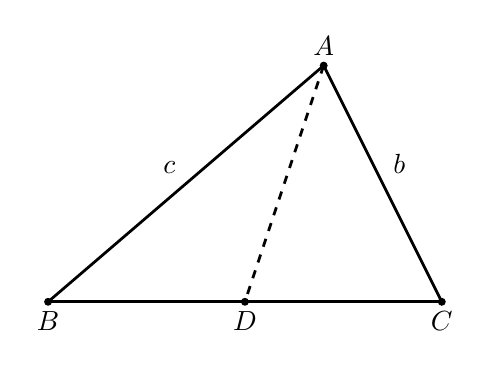
\begin{tikzpicture}[scale=1]
\coordinate[label=below:$D$,] (D) at (0.0,0.0);
\coordinate[label=below:$B$] (B) at (-2.5,0.0);
\coordinate[label=below:$C$] (C) at (2.5,0.0);
\coordinate[label=above:$A$] (A) at (1.0,3.0);
\draw[line width=1pt] (B) to [edge label = $c$] (A);
\draw[line width=1pt] (A) to [edge label = $b$] (C);
\draw[line width=1pt] (C) to (B);
\draw[dashed,line width=1pt] (A) to (D);
\foreach \p in {A,B,C,D}
	\fill[fill=black,draw=black,thick] (\p) circle (1pt);
\end{tikzpicture}
\end{figure*}

\begin{proof}
由余弦定理:
\begin{align*}
AB^2 &= AD^2+BD^2-2AD\cdot BD \cdot \cos\angle ADB, \\
AC^2 &= AD^2+CD^2-2AD\cdot CD \cdot \cos\angle ADC.
\end{align*}
又因为 $BD=CD$, 以及 $\cos\angle ADB=-\cos\angle ADC$, 所以上面两式相加得到:
\[AB^2 + AC^2 = 2(AD^2+BD^2).\]
\end{proof}


%------------------------------------------------------------------------------%
\newpage

\noindent 角平分线的长度关系.

$\triangle ABC$中, $\angle BAC$ 的平分线交 $BC$ 于 $D$. 设 $AB=x$, $AC=y$, $AD=z$, $BD=u$, $CD=v$. 则

(1) $\dfrac{x}{y} = \dfrac{u}{v}$;

(2) $z^2 = xy - uv$.
\begin{figure*}[htbp]
\centering
\begin{tikzpicture}[scale=1]
\coordinate[label=below:$D$,] (D) at (0.351, 0);
\coordinate[label=below:$B$] (B) at (-3,0.0);
\coordinate[label=below:$C$] (C) at (3,0.0);
\coordinate[label=above:$A$] (A) at (1.0,4.0);
\draw[line width=1pt] (B) to [edge label = $x$] (A);
\draw[line width=1pt] (C) to [edge label' = $y$] (A);
\draw[line width=1pt] (B) to [edge label' = $u$] (D);
\draw[line width=1pt] (C) to [edge label = $v$] (D);
\draw[dashed,line width=1pt] (A) to [edge label = $z$] (D);
\foreach \p in {A,B,C,D}
	\fill[fill=black,draw=black,thick] (\p) circle (1pt);
\draw pic["$\alpha$",draw,line width=1pt, angle eccentricity=1.5, angle radius=0.5cm] {angle=B--A--D};
\draw pic["$\alpha$",draw,line width=1pt, angle eccentricity=1.5, angle radius=0.6cm] {angle=D--A--C};
\end{tikzpicture}
\end{figure*}

\begin{proof}
设 $\angle BAD = \angle CAD = \alpha$, 由正弦定理, 
\[\frac{u}{\sin\alpha}=\frac{x}{\sin\angle ADB}, \qquad \frac{v}{\sin\alpha}=\frac{y}{\sin\angle ADC} .\]
并注意到 $\sin\angle ADB = \sin\angle ADC$, 所以有 $\dfrac{x}{y} = \dfrac{u}{v}$.

由余弦定理, 
\begin{align*}
u^2 &= x^2 + z^2 - 2xz\cos\alpha  \\ 
v^2 &= y^2 + z^2 - 2yz\cos\alpha
\end{align*}
设$\dfrac{x}{y} = \dfrac{u}{v} = k$, 则 $x = ky, u = kv$, 代入并令上面二式相减可得
\[ (k^2-1)v^2 = (k^2-1)y^2 - 2(k-1)yz\cos\alpha . \]
可以求出 $2yz\cos\alpha = (k+1)(y^2-v^2)$. 代入 $v^2$ 的表达式得
\[ k(y^2-v^2) = z^2 \]
即
\[z^2 = xy - uv.\]
\end{proof}

%------------------------------------------------------------------------------%
\newpage
托勒密定理: 圆内接四边形两条对角线的乘积等于两对对边乘积之和.

如下图所示, $ABCD$ 为圆内接四边形, 则对角线 $AC$ 与 $BD $ 的乘积等于一对对边 $AB$ 与 $CD$ 的乘积加上另一对对边 $AD$ 与 $BC$ 的乘积, 即 $AC\cdot BD = AB\cdot CD + AD\cdot BC$.

\begin{figure*}[htbp]
\centering
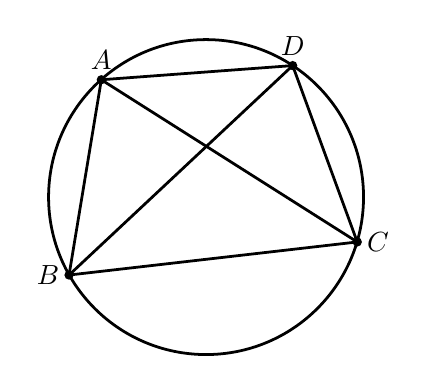
\begin{tikzpicture}[scale=1.0]
\coordinate[] (O) at (0,0);
\coordinate[label=left:$B$] (B) at (-1.74,-0.99);
\coordinate[label=$A$] (A) at (-1.33,1.49);
\coordinate[label=$D$] (D) at (1.1,1.67);
\coordinate[label=right:$C$] (C) at (1.92,-0.57);
\draw [line width=1pt] (O) circle (2cm);
\draw [line width=1pt] (A) -- (B) -- (C) -- (D) -- cycle;
\draw [line width=1pt] (A) -- (C);
\draw [line width=1pt] (B) -- (D);
\foreach \p in {A,B,C,D}
	\fill[fill=black,draw=black,thick] (\p) circle (1.25pt);
\end{tikzpicture}
\end{figure*}

证法1: (构造等角)

不失一般性, 可以假设 $\angle ADB < \angle BDC$, 过点 $D$ 作直线 $DE$ 交 $AC$ 于 $E$, 且满足 $\angle CDE = \angle ADB$, 如下图所示.
\begin{figure*}[htbp]
\centering
\begin{tikzpicture}[scale=1.0]
\coordinate[] (O) at (0,0);
\coordinate[label=left:$B$] (B) at (-1.74,-0.99);
\coordinate[label=$A$] (A) at (-1.33,1.49);
\coordinate[label=$D$] (D) at (1.1,1.67);
\coordinate[label=right:$C$] (C) at (1.92,-0.57);
\coordinate[label=below left:$E$] (E) at (0.62,0.25);
\draw [line width=1pt] (O) circle (2cm);
\draw [line width=1pt] (B) -- (A) -- (D) -- (C) -- cycle;
\draw [line width=1pt] (A) -- (C);
\draw [line width=1pt] (B) -- (D);
\draw [dashed,line width=1pt] (D) -- (E);
\foreach \p in {A,B,C,D,E}
	\fill[fill=black,draw=black,thick] (\p) circle (1.25pt);
\draw pic[draw,line width=1pt, angle eccentricity=1.5, angle radius=0.5cm] {angle=A--D--B};
\draw pic[draw,line width=1pt, angle eccentricity=1.5, angle radius=0.5cm] {angle=E--D--C};
\end{tikzpicture}
\end{figure*}

先证 $\triangle BDA \sim \triangle CDE$. 可以根据 $\angle BDA = \angle CDE$ 和 $\angle ABD = \angle ECD$ 得到. 于是 $AB : CE = BD : CD$, 即 $AB\cdot CD = BD\cdot CE$.

再证 $\triangle DBC \sim \triangle DAE$. 可以根据 $\angle DBC = \angle DAE$ 和 $\angle BDC = \angle ADE$ 得到. 于是 $BD : AD = BC : AE$, 即 $BD\cdot AE = BC\cdot AD$.

两式相加得: $BD\cdot(AE+CE) = AB\cdot CD + AD\cdot BC$, 即 $AC\cdot BD = AB\cdot CD + AD\cdot BC$.

~

证法2: (构造等角)
\begin{figure*}[htbp]
\centering
\begin{tikzpicture}[scale=1.0]
\coordinate[] (O) at (0,0);
\coordinate[label=$A$] (A) at (0,2);
\coordinate[label=above left:$B$] (B) at (-1.78,0.92);
\coordinate[label=right:$C$] (C) at (1.29,-1.53);
\coordinate[label=right:$D$] (D) at (1.51,1.32);
\coordinate[label=left:$P$] (P) at (-3.72,-0.27);
\draw [line width=1pt] (O) circle (2cm);
\draw [line width=1pt] (B) -- (A) -- (D) -- (C) -- cycle;
\draw [line width=1pt] (A) -- (C);
\draw [line width=1pt] (B) -- (D);
\draw [dashed,line width=1pt] (B) -- (P) -- (C);
\foreach \p in {A,B,C,D,P}
	\fill[fill=black,draw=black,thick] (\p) circle (1.25pt);
\draw pic[draw,line width=1pt, angle eccentricity=1.5, angle radius=0.5cm] {angle=D--C--A};
\draw pic[draw,line width=1pt, angle eccentricity=1.5, angle radius=0.5cm] {angle=B--C--P};
\end{tikzpicture}
\end{figure*}

在 $AB$ 的延长线上取一点 $P$, 使得 $\angle BCP = \angle DCA$, 于是 $\angle ACP = \angle DCB$.

再由 $\angle PAC = \angle BDC$, 得 $\triangle ACP\sim\triangle DCB$, 于是$AC:CD = AP:BD$, 即$AC\cdot BD = AP\cdot CD$.

另一方面, 根据 $\angle CBP=180\degree - \angle CBA = \angle CDA$ 和 $\angle BCP=\angle DCA$, 得 $\triangle ACD\sim\triangle PCB$, 于是 $AD:PB=CD:CB$, 即 $AD\cdot CB = CD\cdot BP$.

两式相减得到 $AC\cdot BD - AD \cdot CB = CD(AP-PB)$, 即 $AB\cdot CD+AD\cdot BC = AC\cdot BD$.

~

证法3: (正弦定理)
\begin{figure*}[htbp]
\centering
\begin{tikzpicture}[scale=1.0]
\coordinate[] (O) at (0,0);
\coordinate[label=left:$B$] (B) at (-1.74,-0.99);
\coordinate[label=$A$] (A) at (-1.33,1.49);
\coordinate[label=$D$] (D) at (1.1,1.67);
\coordinate[label=right:$C$] (C) at (1.92,-0.57);
\draw [line width=1pt] (O) circle (2cm);
\draw [line width=1pt] (B) -- (A) -- (D) -- (C) -- cycle;
\draw [line width=1pt] (A) -- (C);
\draw [line width=1pt] (B) -- (D);
\foreach \p in {A,B,C,D}
	\fill[fill=black,draw=black,thick] (\p) circle (1.25pt);
\draw pic["$\alpha$",draw,line width=1pt, angle eccentricity=1.5, angle radius=0.35cm] {angle=B--A--C};
\draw pic["$\alpha$",draw,line width=1pt, angle eccentricity=1.5, angle radius=0.35cm] {angle=B--D--C};
\draw pic["$\beta$",draw,line width=1pt, angle eccentricity=1.5, angle radius=0.35cm] {angle=D--B--A};
\draw pic["$\beta$",draw,line width=1pt, angle eccentricity=1.5, angle radius=0.35cm] {angle=D--C--A};
\draw pic["$\theta$",draw,line width=1pt, angle eccentricity=1.5, angle radius=0.5cm] {angle=A--D--B};
\draw pic["$\theta$",draw,line width=1pt, angle eccentricity=1.5, angle radius=0.5cm] {angle=A--C--B};
\draw pic["$\varphi$",draw,line width=1pt, angle eccentricity=1.5, angle radius=0.5cm] {angle=C--B--D};
\draw pic["$\varphi$",draw,line width=1pt, angle eccentricity=1.5, angle radius=0.5cm] {angle=C--A--D};
\end{tikzpicture}
\end{figure*}

如图, 相等的角用相同的希腊字母表示. 
\[\alpha+\beta+\theta+\varphi=\pi .\]

要证 $AB\cdot CD + BC\cdot AD = AC\cdot BD$, 由正弦定理等价于证
\[\sin\theta \sin\varphi + \sin\alpha \sin\beta = \sin(\alpha+\theta)\sin(\alpha+\varphi).\]
由 $\beta = \pi - (\alpha+\theta+\varphi)$, 则 $\sin\beta = \sin(\alpha+\theta+\varphi)$. 利用和差化积与积化和差将上面的待证等式进行变换.
\begin{align*}
& \sin\theta \sin\varphi + \sin\alpha \sin\beta \\
=& \frac{1}{2}\left[\cos(\theta-\varphi) - \cos(\theta+\varphi)\right]+\frac{1}{2}\left[\cos(\theta+\varphi) - \cos(2\alpha+\theta+\varphi)\right]\\
=& \frac{1}{2}\left[\cos(\theta-\varphi) - \cos(2\alpha+\theta+\varphi)\right]\\
=& \sin(\frac{2\alpha+\theta+\varphi+\theta-\varphi}{2})\sin(\frac{2\alpha+\theta+\varphi+\varphi-\theta}{2})\\
=& \sin(\alpha+\theta)\sin(\alpha+\varphi).
\end{align*}

~

证法4: (余弦定理)
\begin{figure*}[htbp]
\centering
\begin{tikzpicture}[scale=1.0]
\coordinate[] (O) at (0,0);
\coordinate[label=left:$B$] (B) at (-1.74,-0.99);
\coordinate[label=$A$] (A) at (-1.33,1.49);
\coordinate[label=$D$] (D) at (1.1,1.67);
\coordinate[label=right:$C$] (C) at (1.92,-0.57);
\draw [line width=1pt] (O) circle (2cm);
\draw [line width=1pt] (A) to[edge label'=$a$](B);
\draw [line width=1pt] (B) to[edge label'=$b$](C);
\draw [line width=1pt] (C) to[edge label'=$c$](D);
\draw [line width=1pt] (D) to[edge label'=$d$](A);
\draw [line width=1pt] (A) -- (C) node [near end,above] {$m$};
\draw [line width=1pt] (B) to[edge label'=$n$] (D);
\foreach \p in {A,B,C,D}
	\fill[fill=black,draw=black,thick] (\p) circle (1.25pt);
\draw pic["$\theta$",draw,line width=1pt, angle eccentricity=1.5, angle radius=0.5cm] {angle=C--B--A};
\end{tikzpicture}
\end{figure*}

如图, 设 $AB=a, BC=b, CD=c, DA=d, AC=m, BD=n, \angle ABC=\theta$.

在 $\triangle ABC$ 和 $\triangle ADC$ 中, 由余弦定理有:
\begin{align*}
m^2 &= a^2+b^2-2ab\cos\theta \qquad\cdots\qquad \raisebox{.5pt}{\textcircled{\raisebox{0pt} {1}}} \\
m^2 &= c^2+d^2+2cd\cos\theta \qquad\cdots\qquad \raisebox{.5pt}{\textcircled{\raisebox{0pt} {2}}}
\end{align*}
由 $\raisebox{.5pt}{\textcircled{\raisebox{0pt} {1}}}\times cd + \raisebox{.5pt}{\textcircled{\raisebox{0pt} {2}}}\times ab$ 得:
\begin{align*} 
(ab+cd)m^2 &= cd(a^2+b^2)+ab(c^2+d^2) \\
&= (ac+bd)(ad+bc)
\end{align*}
于是
\[ m^2 = \frac{(ac+bd)(ad+bc)}{ab+cd} .\]
同理, 
\[n^2 =  \dfrac{(ac+bd)(ab+cd)}{ad+bc} .\]
相乘可得: $(mn)^2=(ac+bd)^2$. 所以 $AB\cdot CD+BC\cdot AD=AC\cdot BD$.

~

证法5: (面积法)

\begin{figure*}[htbp]
\centering
\begin{tikzpicture}[scale=1.0]
\coordinate[] (O) at (0,0);
\coordinate[label=$A$] (A) at (0.33,1.97);
\coordinate[label=left:$B$] (B) at (-1.9,-0.62);
\coordinate[label=below:$C$] (C) at (0.55,-1.92);
\coordinate[label=right:$D$] (D) at (1.69,1.08);
\coordinate[label=left:$E$] (E) at (-1.73,1.0);
\coordinate[label=right:$F$] (F) at (0.41,0.47);
\draw [line width=1pt] (O) circle (2cm);
\draw [line width=1pt] (A) -- (B) -- (C) -- (D) -- cycle;
\draw [line width=1pt] (A) -- (C);
\draw [line width=1pt] (B) -- (D);
\draw [dashed,line width=1pt] (A) -- (E) -- (B);
\draw [dashed,line width=1pt] (C) -- (E) -- (D);
\foreach \p in {A,B,C,D,E,F}
	\fill[fill=black,draw=black,thick] (\p) circle (1.25pt);
\draw pic["$\alpha$",draw,line width=1pt, angle eccentricity=1.5, angle radius=0.4cm] {angle=D--B--A};
\draw pic["$\alpha$",draw,line width=1pt, angle eccentricity=1.5, angle radius=0.4cm] {angle=E--D--B};
\draw pic["$\beta$",draw,line width=1pt, angle eccentricity=1.5, angle radius=0.45cm] {angle=B--A--C};
\draw pic["$\beta$",draw,line width=1pt, angle eccentricity=1.5, angle radius=0.45cm] {angle=B--D--C};
\end{tikzpicture}
\end{figure*}

如图, $AB,CD$的交点记为$F$, 作 $AE$ 平行于 $BD$ 交圆与 $E$ 点, 并连接 $BE, CE, DE$. 于是四边形 $AEBD$ 为等腰梯形, $EB = AD$. 图中相等得角用相同得希腊字母标出. 易知 $\angle AFD = \alpha+\beta=\angle EDC$.

记四边形$ABCD$的面积为 $S_1$, 四边形$EBCD$的面积为 $S_2$. 则
\begin{align*}
S_1 &= S_{\triangle ABD} + S_{\triangle BCD}\\
&= \frac{1}{2} BD \cdot AF \sin\angle AFD + \frac{1}{2} BD \cdot CF \sin\angle BFC\\
&= \frac{1}{2} BD\cdot AC \sin\angle AFD \\
&= \frac{1}{2} BD\cdot AC \sin\angle EDC \\
S_2 &= S_{\triangle EBC} + S_{\triangle EDC}\\
&= \frac{1}{2} EB \cdot BC \sin\angle EBC + \frac{1}{2} ED \cdot CD \sin\angle EDC
\end{align*}
因为 $\angle EBC$ 与 $\angle EDC$ 互补, 所以 $\sin\angle EBC = \sin\angle EDC$; 再由 $EB=AD$, $ED=AB$, 代入 $S_2$表达式得到:
\[ S_2 = \frac{1}{2}(AD\cdot BC + AB\cdot CD)\sin\angle EDC .\]

另一方面, $S_1 = S_{\triangle ABD} + S_{\triangle BCD} = S_{\triangle EBD} + S_{\triangle BCD} = S_2$, 所以 $AD\cdot BC + AB\cdot CD = AC\cdot BD$.

~

证法6: (无字证明)
\begin{figure*}[htbp]
\centering
\begin{minipage}[t]{0.4\linewidth}
\begin{tikzpicture}[scale=1.0]
\coordinate[] (O) at (0,0);
\coordinate[label=left:$A$] (A) at (-1.91,-0.6);
\coordinate[label=above:$B$] (B) at (-0.62,1.9);
\coordinate[label=right:$C$] (C) at (1.91,-0.6);
\coordinate[label=below:$D$] (D) at (0,-2);
\draw [line width=1pt] (O) circle (2cm);
\draw [line width=1pt] (A) -- (B) node [midway,above,sloped] {$a$};
\draw [line width=1pt] (B) -- (C) node [midway,above,sloped] {$b$};
\draw [line width=1pt] (C) -- (D) node [midway,above,sloped] {$c$};
\draw [line width=1pt] (D) -- (A) node [midway,above,sloped] {$d$};
\draw [line width=1pt] (A) -- (C) node [near start,above,sloped] {$e$};
\draw [line width=1pt] (B) -- (D) node [midway,below,sloped] {$f$};
\foreach \p in {A,B,C,D}
	\fill[fill=black,draw=black,thick] (\p) circle (1.25pt);
\draw pic["$\beta$",draw,line width=1pt, angle eccentricity=1.8, angle radius=0.35cm] {angle=C--A--B};
\draw pic["$\beta$",draw,line width=1pt, angle eccentricity=1.8, angle radius=0.35cm] {angle=C--D--B};
\draw pic["$\delta$",draw,line width=1pt, angle eccentricity=1.8, angle radius=0.35cm] {angle=A--B--D};
\draw pic["$\delta$",draw,line width=1pt, angle eccentricity=1.8, angle radius=0.35cm] {angle=A--C--D};
\draw pic["$\alpha$",draw,line width=1pt, angle eccentricity=1.5, angle radius=0.5cm] {angle=B--D--A};
\draw pic["$\alpha$",draw,line width=1pt, angle eccentricity=1.5, angle radius=0.5cm] {angle=B--C--A};
\draw pic["$\gamma$",draw,line width=1pt, angle eccentricity=1.5, angle radius=0.5cm] {angle=D--B--C};
\draw pic["$\gamma$",draw,line width=1pt, angle eccentricity=1.5, angle radius=0.5cm] {angle=D--A--C};
\node at (0,-3.0) {$\alpha+\beta+\gamma+\delta=\pi$};
\end{tikzpicture}
\end{minipage}
\begin{minipage}[t]{0.5\linewidth}
\begin{tikzpicture}[scale=1.35]
\coordinate[] (A) at (0,0);
\coordinate[] (B) at (4,0);
\coordinate[] (C) at (3.57,2.63);
\coordinate[] (D) at (-0.43,2.63);
\coordinate[] (E) at (1.35,2.63);
\draw [line width=1pt] (A) -- (B) node [midway,below,sloped] {$e\cdot f$};
\draw [line width=1pt] (B) to[edge label'=$a\cdot b$] (C);
\draw [line width=1pt] (C) -- (E) node [midway,above,sloped] {$b\cdot d$};
\draw [line width=1pt] (E) -- (D) node [midway,above,sloped] {$a\cdot c$};
\draw [line width=1pt] (D) to[edge label'=$a\cdot b$] (A);
\draw [line width=1pt] (A) to[edge label'=$a\cdot f$] (E);
\draw [line width=1pt] (E) to[edge label'=$b\cdot f$] (B);
\foreach \p in {A,B,C,D,E}
	\fill[fill=black,draw=black,thick] (\p) circle (1.25pt);
\draw pic["$\alpha+\delta$",draw,line width=1pt, angle eccentricity=2.2, angle radius=0.35cm] {angle=A--D--E};
\draw pic["$\beta$",draw,line width=1pt, angle eccentricity=1.8, angle radius=0.35cm] {angle=D--E--A};
\draw pic["$\gamma$",draw,line width=1pt, angle eccentricity=1.8, angle radius=0.35cm] {angle=E--A--D};
\draw pic["$\beta$",draw,line width=1pt, angle eccentricity=1.8, angle radius=0.45cm] {angle=B--A--E};
\draw pic["$\gamma+\delta$",draw,line width=1pt, angle eccentricity=1.8, angle radius=0.45cm] {angle=A--E--B};
\draw pic["$\alpha$",draw,line width=1pt, angle eccentricity=1.8, angle radius=0.45cm] {angle=E--B--A};
\draw pic["$\alpha$",draw,line width=1pt, angle eccentricity=1.8, angle radius=0.35cm] {angle=B--E--C};
\draw pic["$\delta$",draw,line width=1pt, angle eccentricity=1.8, angle radius=0.35cm] {angle=C--B--E};
\draw pic["$\beta+\gamma$",draw,line width=1pt, angle eccentricity=2.0, angle radius=0.35cm] {angle=E--C--B};
\node at (2,-1.0) {$a\cdot c+b\cdot d=e\cdot f$};
\end{tikzpicture}
\end{minipage}
\end{figure*}

~

证法7: (复数法)
\begin{figure*}[htbp]
\centering
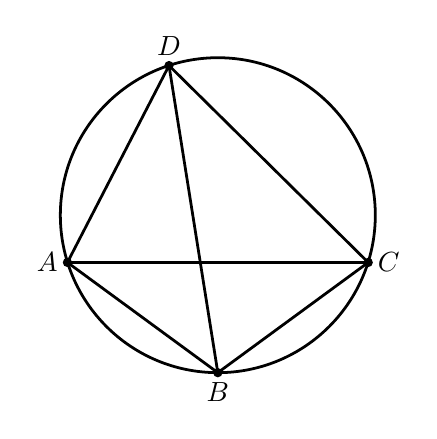
\begin{tikzpicture}[scale=1.0]
\coordinate[] (O) at (0,0);
\coordinate[label=left:$A$] (A) at (-1.91,-0.6);
\coordinate[label=above:$D$] (D) at (-0.62,1.9);
\coordinate[label=right:$C$] (C) at (1.91,-0.6);
\coordinate[label=below:$B$] (B) at (0,-2);
\draw [line width=1pt] (O) circle (2cm);
\draw [line width=1pt] (A) -- (B) -- (C) -- (D) -- cycle;
\draw [line width=1pt] (A) -- (C);
\draw [line width=1pt] (B) -- (D);
\foreach \p in {A,B,C,D}
	\fill[fill=black,draw=black,thick] (\p) circle (1.25pt);
\end{tikzpicture}
\end{figure*}

用 $a,b,c,d$ 分别表示 $A,B,C,D$ 的复数. 则
\begin{align*}
%overrightarrow
\vec{AB} &= b-a, \qquad \vec{AD} = d-a, \qquad \vec{AC} = c-a, \\
\vec{CD} &= d-c, \qquad \vec{BC} = c-b, \qquad \vec{BD} = d-b. 
\end{align*}
考虑到 
\begin{align*}
\angle DAB &= \arg\vec{AD}-\arg\vec{AB}\\
 &= \arg(d-a) - \arg(b-a)\\
\angle DCB &= 2\pi - (\arg\vec{CD} - \arg\vec{CB})\\
&= \arg(b-c)-\arg(d-c) + 2\pi
\end{align*}
由 $\angle DAB + \angle DCB = \pi$, 将上两式相加得:
\[\arg(d-a) - \arg(b-a) + \arg(b-c)-\arg(d-c) + \pi = 0\]
移项并注意到对于任意复数 $z$, $\arg(z)\pm\pi = \arg(-z)$, 得:
\[\arg(d-a) + \arg(c-b) = \arg(b-a) + \arg(d-c) \]
由辐角公式推出:
\[\arg[(d-a)(c-b)] = \arg[(b-a)(d-c)].\]
这表明两个复数$(d-a)(c-b)$和$(b-a)(d-c)$共线且同向, 于是模长之和等于和的模长:
\begin{align*}
|(b-a)(d-c)| + |(d-a)(c-b)| &= |(b-a)(d-c)+(d-a)(c-b)|\\
&= |(c-a)(d-b)|
\end{align*}
复数模长的乘积等于乘积的模长, 上面的等式就是
\[|\vec{AB}|\cdot|\vec{CD}| + |\vec{AD}|\cdot|\vec{BC}| = |\vec{AC}|\cdot|\vec{BD}|\]

~

证法8: (反演变换)
\begin{figure*}[htbp]
\centering
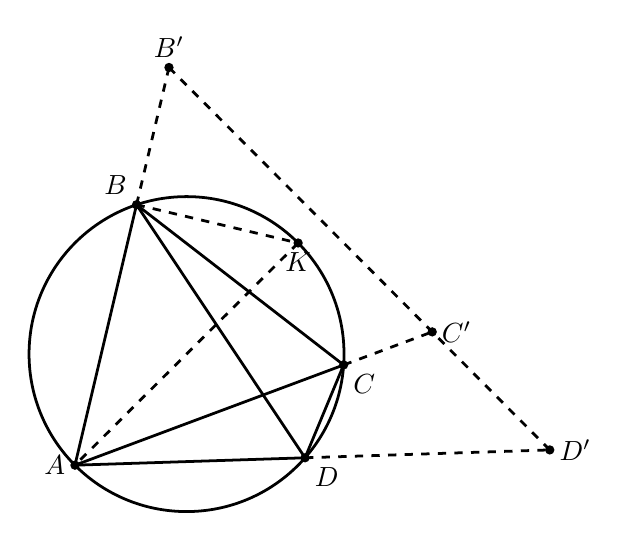
\begin{tikzpicture}[scale=1.0]
\coordinate[] (O) at (0,0);
\coordinate[label=left:$A$] (A) at (-1.417,-1.411);
\coordinate[label=above left:$B$] (B) at (-0.635,1.897);
\coordinate[label=below right:$C$] (C) at (1.995,-0.138);
\coordinate[label=below right:$D$] (D) at (1.505,-1.317);
\coordinate[label=above:$B'$] (BB) at (-0.223,3.64);
\coordinate[label=right:$C'$] (CC) at (3.12, 0.282);
\coordinate[label=right:$D'$] (DD) at (4.613, -1.217);
\coordinate[label=below:$K$] (K) at (1.417,1.411);
\draw [line width=1pt] (O) circle (2cm);
\draw [line width=1pt] (A) -- (B) -- (C) -- (D) -- cycle;
\draw [line width=1pt] (A) -- (C);
\draw [line width=1pt] (B) -- (D);
\draw [dashed,line width=1pt] (B) -- (BB);
\draw [dashed,line width=1pt] (C) -- (CC);
\draw [dashed,line width=1pt] (D) -- (DD);
\draw [dashed,line width=1pt] (BB) -- (DD);
\draw [dashed,line width=1pt] (B) -- (K) -- (A);
\foreach \p in {A,B,C,D,BB,CC,DD,K}
	\fill[fill=black,draw=black,thick] (\p) circle (1.25pt);
\end{tikzpicture}
\end{figure*}

对 $B,C,D$ 三点分别做反演变换, 反演变换的圆心为点 $A$, 半径为 1, 变换后得到的点为 $B', C', D'$. 则:
\[ AB\cdot AB'=AC\cdot AC'=AD\cdot AD'=1 .\]
由余弦定理:
\begin{align*}
C'D' &= \sqrt{AC'^2 + AD'^2 - 2AC'\cdot AD'\cos\angle CAD}\\
&= \sqrt{AC^2 + AD^2-2AC\cdot AD\cos\angle CAD}\cdot\left(\frac{1}{AC}\cdot\frac{1}{AD}\right)\\
&= \frac{CD}{AC\cdot AD} .
\end{align*}
同理可得: \[B'C' = \dfrac{BC}{AB\cdot AC}, B'D'=\dfrac{BD}{AB\cdot AD} .\]
因为 $A,B,C,D$ 共圆, 所以 $B',C',D'$共线, 于是有: $B'C'+C'D'=B'D'$, 即:
\[\frac{BC}{AB\cdot AC}+\frac{CD}{AC\cdot AD} = \frac{BD}{AB\cdot AD}.\]
两边都乘以 $AB\cdot AC\cdot AD$ 得: $BC\cdot AD+ AB\cdot CD = BD\cdot AC$.

~

补充: 类似的思路, 但不需要用反演的性质, 可以用向量的方法, 在 $AB, AC, AD$的延长线上分别取  $B',C',D'$, 满足 $\vec{AB}\cdot\vec{AB'}=\vec{AC}\cdot\vec{AC'}=\vec{AD}\cdot\vec{AD'}=1$. 下面证明 $B',C',D'$ 共线. 

设 $AK$ 是圆 $ABCD$ 的直径, 则$AB\perp BK$, 向量 $\vec{AK}$ 在 $AB$ 上的投影就是 $\vec{AB}$, 故 $\vec{AK}\cdot\vec{AB'}=1$. 同理也有 $\vec{AK}\cdot\vec{AC'}=\vec{AK}\cdot\vec{AD'}=1$. 于是有 $\vec{AK}\cdot(\vec{AC'}-\vec{AB'}) = \vec{AK}\cdot\vec{B'C'} = 0$ 和 $\vec{AK}\cdot(\vec{AD'}-\vec{AC'}) = \vec{AK}\cdot\vec{C'D'} = 0$, 说明 $\vec{B'C'}, \vec{C'D'}$ 都垂直于 $\vec{AK}$, 所以 $B'C'D'$ 共线. 

剩余部分用反演法中的余弦定理往下推导即可.

~

证法9: (向量法)
\begin{figure*}[htbp]
\centering
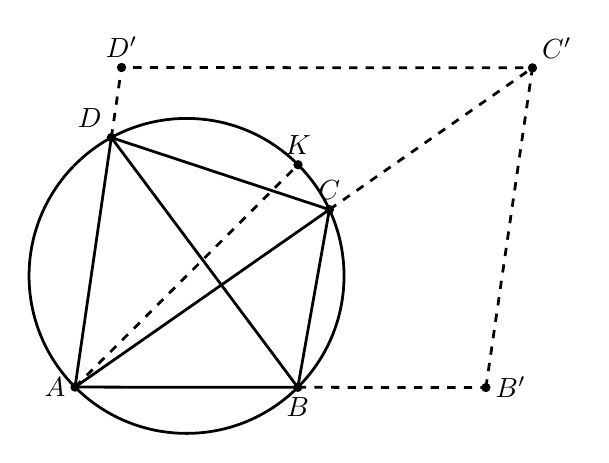
\begin{tikzpicture}[scale=1.0]
\coordinate[] (O) at (0,0);
\coordinate[label=left:$A$] (A) at (-1.416,-1.412);
\coordinate[label=below:$B$] (B) at (1.413,-1.415);
\coordinate[label=above:$C$] (C) at (1.814,0.842);
\coordinate[label=above left:$D$] (D) at (-0.955,1.757);
\coordinate[label=right:$B'$] (BB) at (3.802,-1.418);
\coordinate[label=above right:$C'$] (CC) at (4.393, 2.642);
\coordinate[label=above:$D'$] (DD) at (-0.825, 2.647);
\coordinate[label=above:$K$] (K) at (1.416,1.412);
\draw [line width=1pt] (O) circle (2cm);
\draw [line width=1pt] (A) -- (B) -- (C) -- (D) -- cycle;
\draw [line width=1pt] (A) -- (C);
\draw [line width=1pt] (B) -- (D);
\draw [dashed,line width=1pt] (B) -- (BB);
\draw [dashed,line width=1pt] (C) -- (CC);
\draw [dashed,line width=1pt] (D) -- (DD);
\draw [dashed,line width=1pt] (BB) -- (CC) -- (DD);
\draw [dashed,line width=1pt] (A) -- (K);
\foreach \p in {A,B,C,D,BB,CC,DD,K}
	\fill[fill=black,draw=black,thick] (\p) circle (1.25pt);
\end{tikzpicture}
\end{figure*}

在 $AB, AC, CD$ 上各取一点 $B',C',D'$, 使得$AB'C'D'$是平行四边形. 由 $\angle C'AB' = \angle CDB$ 和 $\angle AC'B' = \angle C'AD = \angle DBC$, 得 $\triangle C'AB'\sim\triangle BDC$, 所以
\[\frac{|\vec{BD}|}{|\vec{AC'}|} = \frac{|\vec{CD}|}{|\vec{AB'}|} = \frac{|\vec{BC}|}{|\vec{B'C'}|} \qquad\cdots\qquad \raisebox{.5pt}{\textcircled{\raisebox{0pt} {1}}}.\]

设 $AK$ 是圆的直径, 所以$\vec{AK}$ 在$AB,AC,AD$上的投影分别是$\vec{AB},\vec{AC},\vec{AD}$, 于是
\begin{align*}
\vec{AC}\cdot\vec{AC'} &= \vec{AF}\cdot\vec{AC'} = \vec{AK}\cdot(\vec{AB'}+\vec{AD'})\\
&= \vec{AK}\cdot\vec{AB'}+\vec{AK}\cdot\vec{AD'}\\
&= \vec{AB}\cdot\vec{AB'}+\vec{AD}\cdot\vec{AD'}
\end{align*}
即: \[|\vec{AC}|\cdot|\vec{AC'}| = |\vec{AB}|\cdot|\vec{AB'}| + |\vec{AD}|\cdot|\vec{AD'}| .\]
上式乘以$\raisebox{.5pt}{\textcircled{\raisebox{0pt} {1}}}$式得: 
\[|\vec{AC}|\cdot|\vec{AC'}|\cdot\frac{|\vec{BD}|}{|\vec{AC'}|} = |\vec{AB}|\cdot|\vec{AB'}|\cdot\frac{|\vec{CD}|}{|\vec{AB'}|} + |\vec{AD}|\cdot|\vec{AD'}|\cdot\frac{|\vec{BC}|}{|\vec{B'C'}|} .\]
注意到 $\vec{B'C'}=\vec{AD'}$, 所以 $|\vec{AC}|\cdot|\vec{BD}| = |\vec{AB}|\cdot|\vec{CD}|+|\vec{AD}|\cdot|\vec{BC}|$.

~

证法10: (坐标解析法, 本质是正弦定理)
\begin{figure*}[htbp]
\centering
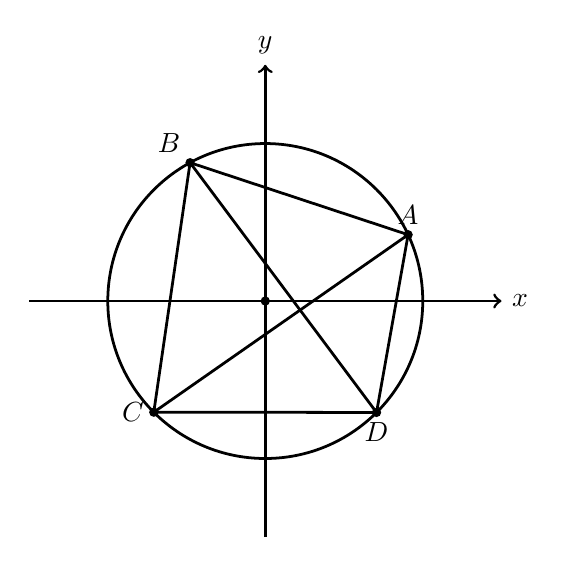
\begin{tikzpicture}[scale=1.0]
\tikzstyle{axes}=[line width=1pt]
\coordinate[] (O) at (0,0);
\coordinate[label=above:$A$] (A) at (1.814,0.842);
\coordinate[label=above left:$B$] (B) at (-0.955,1.757);
\coordinate[label=left:$C$] (C) at (-1.416,-1.412);
\coordinate[label=below:$D$] (D) at (1.413,-1.415);
\draw [line width=1pt] (O) circle (2cm);
\draw [line width=1pt] (A) -- (B) -- (C) -- (D) -- cycle;
\draw [line width=1pt] (A) -- (C);
\draw [line width=1pt] (B) -- (D);
\begin{scope}[style=axes]
    \draw[->] (-3,0) -- (3,0) node[right] {$x$};
    \draw[->] (0,-3) -- (0,3) node[above] {$y$};
\end{scope}
\foreach \p in {A,B,C,D,O}
	\fill[fill=black,draw=black,thick] (\p) circle (1.25pt);
\end{tikzpicture}
\end{figure*}

设圆的半径为1, $A,B,C,D$ 四点的坐标分别是 $A=(\cos\alpha,\sin\alpha)$, $B=(\cos\beta,\sin\beta)$, $C=(\cos\gamma,\sin\gamma)$, $D=(\cos\delta,\sin\delta)$, 其中 $\alpha<\beta<\gamma<\delta$. 由正弦定理可得: 
\begin{align*}
|AB| &= 2\sin(\frac{\beta-\alpha}{2}),\qquad |CD| = 2\sin(\frac{\delta-\gamma}{2}), \\
|AD| &= 2\sin(\frac{\delta-\alpha}{2}), \qquad |BC| = 2\sin(\frac{\gamma-\beta}{2}),\\
|AC| &= 2\sin(\frac{\gamma-\alpha}{2}), \qquad |BD| = 2\sin(\frac{\delta-\beta}{2}).
\end{align*}
进而:
\begin{align*}
&|AB|\cdot|CD|+|AD|\cdot|BC| \\
=& 4\sin(\frac{\beta-\alpha}{2})\sin(\frac{\delta-\gamma}{2}) + 4\sin(\frac{\delta-\alpha}{2})\sin(\frac{\gamma-\beta}{2}) \\
=& 2\cos(\frac{\beta-\alpha-\delta+\gamma}{2}) - 2\cos(\frac{\delta-\alpha+\gamma-\beta}{2})\\
=&4\sin(\frac{\gamma-\alpha}{2})\sin(\frac{\delta-\beta}{2})\\
=&|AC|\cdot|BD|
\end{align*}

~

证法11: (反演变换2.0)
\begin{figure*}[htbp]
\centering
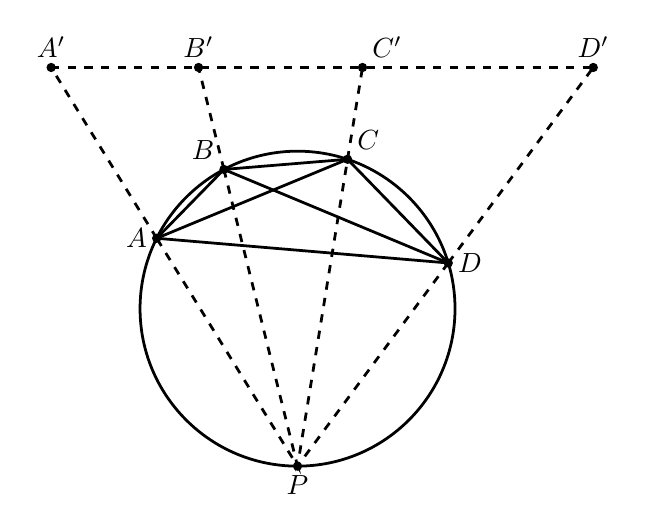
\begin{tikzpicture}[scale=1.0]
\coordinate[] (O) at (0,0);
\coordinate[label=left:$A$] (A) at (-1.789,0.894);
\coordinate[label=above left:$B$] (B) at (-0.935,1.768);
\coordinate[label=above right:$C$] (C) at (0.635,1.897);
\coordinate[label=right:$D$] (D) at (1.914,0.58);
\coordinate[label=above:$A'$] (AA) at (-3.129,3.063);
\coordinate[label=above:$B'$] (BB) at (-1.257,3.063);
\coordinate[label=above right:$C'$] (CC) at (0.825, 3.063);
\coordinate[label=above:$D'$] (DD) at (3.756, 3.063);
\coordinate[label=below:$P$] (P) at (0, -2);
\draw [line width=1pt] (O) circle (2cm);
\draw [line width=1pt] (A) -- (B) -- (C) -- (D) -- cycle;
\draw [line width=1pt] (A) -- (C);
\draw [line width=1pt] (B) -- (D);
\draw [dashed,line width=1pt] (B) -- (P) -- (A);
\draw [dashed,line width=1pt] (D) -- (P) -- (C);
\draw [dashed,line width=1pt] (A) -- (AA);
\draw [dashed,line width=1pt] (B) -- (BB);
\draw [dashed,line width=1pt] (C) -- (CC);
\draw [dashed,line width=1pt] (D) -- (DD);
\draw [dashed,line width=1pt] (AA) -- (BB) -- (CC) -- (DD);
\foreach \p in {A,B,C,D,AA,BB,CC,DD,P}
	\fill[fill=black,draw=black,thick] (\p) circle (1.25pt);
\end{tikzpicture}
\end{figure*}

在圆上取不同于 $A,B,C,D$ 的一点 $P$, 对$A,B,C,D$分别作反演变换, 反演中心为 $P$, 半径为 1. 则
\[ PA\cdot PA'=PB\cdot PB'=PC\cdot PC'=PD\cdot PD'=1 .\]
考虑 $\triangle PAB$ 和 $\triangle PB'A'$, 因为 $PA:PB = PB':PA'$, 再加上一个公共角 $\angle A'PB'=\angle BPA$, 所以 $\triangle PAB \sim \triangle PB'A'$, 故 $A'B':BA = PA':PB$, 于是
\[ A'B' = \frac{AB\cdot PA'}{PB} = \frac{AB}{PA\cdot PB} .\]
同理还有
\begin{align*}
A'C' &= \frac{AC}{PA\cdot PC}, \qquad A'D' = \frac{AD}{PA\cdot PD}, \qquad B'C' = \frac{BC}{PB\cdot PC}\\
C'D' &= \frac{CD}{PC\cdot PD}, \qquad B'D' = \frac{BD}{PB\cdot PD} .
\end{align*}
由反演性质知$A',B',C',D'$共线, 所以
\begin{align*}
A'C'\cdot B'D' &= (A'B'+B'C')\cdot(B'C'+C'D')\\
&=A'B'\cdot C'D'+B'C'\cdot(A'B'+B'C'+C'D')\\
&=A'B'\cdot C'D'+B'C'\cdot A'D'
\end{align*}
将上面各式代入后, 并约去分母, 得到: $AC\cdot BD = AB\cdot CD+BC\cdot AD$.

~

证法12: (余弦定理)
\begin{figure*}[htbp]
\centering
\begin{tikzpicture}[scale=1.0]
\coordinate[] (O) at (0,0);
\coordinate[label=right:$A$] (A) at (1.595,1.207);
\coordinate[label=above left:$B$] (B) at (-0.794,1.836);
\coordinate[label=left:$C$] (C) at (-1.869,-0.711);
\coordinate[label=below right:$D$] (D) at (1.789,-0.894);
\coordinate[label=below:$P$] (P) at (0.417,0.555);
\draw [line width=1pt] (O) circle (2cm);
\draw [line width=1pt] (A) -- (B) -- (C) -- (D) -- cycle;
\draw [line width=1pt] (A) -- (P) node [midway,above,sloped] {$x$};
\draw [line width=1pt] (P) -- (C) node [midway,below,sloped] {$K/x$};
\draw [line width=1pt] (B) -- (P) node [midway,below,sloped] {$K/y$};
\draw [line width=1pt] (P) -- (D)  node [midway,below,sloped] {$y$};
\foreach \p in {A,B,C,D,P}
	\fill[fill=black,draw=black,thick] (\p) circle (1.25pt);
\draw pic["$\alpha$",draw,line width=1pt, angle eccentricity=2.0, angle radius=0.35cm] {angle=D--P--A};
\end{tikzpicture}
\end{figure*}

设 $AC, BD$ 交于 $P$ 点, $\angle APD = \alpha$. 设 $PA=x, PD=y$, 由圆幂定理得
\[PA\cdot PC = PB\cdot PD = K, \]
于是 $PB = \dfrac{K}{y}, PC = \dfrac{K}{x}$. 由余弦定理:
\begin{align*}
AD &= \sqrt{x^2+y^2-2xy\cdot\cos\alpha}\\
BC &= \frac{K}{xy}\sqrt{x^2+y^2-2xy\cdot\cos\alpha}\\
AB &= \sqrt{x^2+\frac{K^2}{y^2}+2x\cdot\frac{K}{y}\cdot\cos\alpha}\\
CD &= \frac{y}{x}\sqrt{x^2+\frac{K^2}{y^2}+2x\cdot\frac{K}{y}\cdot\cos\alpha}\\
AC&= x + \frac{K}{x} , \qquad BD = y + \frac{K}{y}
\end{align*}
进而:
\begin{align*}
AB\cdot CD &= \frac{y}{x}(x^2+\frac{K^2}{y^2}+2x\cdot\frac{K}{y}\cdot\cos\alpha) = xy+\frac{K^2}{xy}+2K\cdot\cos\alpha\\
AD\cdot BC &= \frac{K}{xy}(x^2+y^2-2xy\cdot\cos\alpha) = \frac{Kx}{y} + \frac{Ky}{x}-2K\cdot\cos\alpha \\
AB\cdot CD + AD\cdot BC &= K\cdot\frac{x}{y} + K\cdot\frac{y}{x} + xy + \frac{K^2}{xy}\\
&= (x+\frac{K}{x})(y+\frac{K}{y})\\
&= AC\cdot BD
\end{align*}

~

证法13: (函数求导)
\begin{figure*}[htbp]
\centering
\begin{tikzpicture}[scale=1.0]
\coordinate[] (O) at (0,0);
\coordinate[label=right:$A$] (A) at (1.741,0.984);
\coordinate[label=above left:$B$] (B) at (-0.894,1.789);
\coordinate[label=left:$C$] (C) at (-1.917,-0.57);
\coordinate[label=below right:$D$] (D) at (1.621,-1.172);
\coordinate[label=above:$E$] (E) at (0.599,1.333);
\coordinate[label=left:$F$] (F) at (-1.22,1.037);
\coordinate[label=below:$G$] (G) at (0.088,-0.911);
\coordinate[label=right:$H$] (H) at (1.703,0.297);
\coordinate[label=right:$P$] (P) at (0.307,0.375);
\draw [line width=1pt] (O) circle (2cm);
\draw [line width=1pt] (A) -- (B) -- (C) -- (D) -- cycle;
\draw [line width=1pt] (A) -- (C);
\draw [line width=1pt] (B) -- (D);
\draw [dashed,line width=1pt] (P) -- (E) -- (F) -- cycle;
\foreach \p in {A,B,C,D,E,F,G,H,P}
	\fill[fill=black,draw=black,thick] (\p) circle (1.25pt);
\draw pic["$\alpha$",draw,line width=1pt, angle eccentricity=2.0, angle radius=0.35cm] {angle=C--P--D};
\tkzMarkRightAngle[line width=1pt](P,E,A);
\tkzMarkRightAngle[line width=1pt](P,F,C);
\end{tikzpicture}
\end{figure*}

设 $AC, BD$ 的交点为 $P$, 固定 $PA,PB,PC,PD$ 的长度, $AC$ 不动, $BD$ 绕着 $P$ 点旋转, 因为恒有 $PA\cdot PC = PB\cdot PD$, 所以 $A,B,C,D$ 四点总是共圆的. 过 $P$ 点作 $AB,BC,CD,DA$ 的垂线, 垂足分别为 $E,F,G,H$.

设 $\angle APB = \alpha$, 则四条边 $AB,BC,CD,DA$ 的长度各自是 $\alpha$ 的一元函数. 例如
\[ AB^2 = PA^2 + PB^2 - 2PA\cdot PB\cdot\cos\alpha .\]
两边对 $\alpha$ 求导:
\[2AB\cdot AB'(\alpha) = 2PA\cdot PB\sin\alpha ,\]
即 $AB'(\alpha) = \dfrac{PA\cdot PB\sin\alpha}{AB}$, 说明 $AB'(\alpha)$ 等于 $P$ 到 $AB$ 的距离, 即 $AB'(\alpha) = PE$. 

同理, $CD'(\alpha)=PG$. $PB$与$PC$的夹角为 $\pi-\alpha$, 容易得到 $BC'(\alpha)=-PF, AD'(\alpha)=PH$.
最后, $AC$ 和 $BD$ 的长度不随 $\alpha$ 变化, 所以 $AC'(\alpha)=BD'(\alpha)=0$.

令 $f(\alpha) = AB\cdot CD + AD\cdot BC - AC\cdot BD$, 则
\begin{align*} f' &= AB'\cdot CD +AB\cdot CD'+ AD'\cdot BC +AD\cdot BC' - AC'\cdot BD-AC\cdot BD'\\
&= PE\cdot CD + AB\cdot PG - PH\cdot BC - AD\cdot PF
\end{align*}
由 $\triangle ABP \sim \triangle DCP$, 得 $PE:PG = AB:CD$, 即 $PE\cdot CD = PG\cdot AB$. 同理由 $\triangle BCP \sim \triangle ADP$, 可得 $PF\cdot AD = PH\cdot BC$. 于是
\[ f' = 2(PE\cdot CD - PF\cdot AD) .\]
考虑四边形 $PEBF$, 因为有一组对角都是直角, 所以 $P,E,B,F$ 四点共圆, 由 $\angle EFP = \angle ADB = \angle ACD$, 以及 $\angle FEP = \angle CBD = \angle CAD$, 推出 $\triangle EFP\sim\triangle ACD$, 于是 $PE\cdot CD = PF\cdot AD$. 这说明 $f'(\alpha) = 0$, 所以 $f(\alpha)$ 不随 $\alpha$ 变化.

特别地, 取 $\alpha = 0$, 则 $A,B,C,D$ 共线, 沿着$C$到 $A$ 方向上四个点经过的顺序依次是 $C,D,A,B$, 所以
\begin{align*}
f(0) &= AB\cdot CD + AD\cdot BC - AC\cdot BD\\
&= AB\cdot CD + AD\cdot(CD+AD+AB) - (CD+AD)\cdot(AD+AB)
&=0
\end{align*}
这就证明了 $AB\cdot CD + AD\cdot BC = AC\cdot BD$.

~

证法14: (面积法 2.0)
\begin{figure*}[htbp]
\centering
\begin{tikzpicture}[scale=1.0]
\coordinate[] (O) at (0,0);
\coordinate[label=right:$A$] (A) at (2,0);
\coordinate[label=below right:$B$] (B) at (1.643,-1.14);
\coordinate[label=below left:$C$] (C) at (-1.347,-1.478);
\coordinate[label=above left:$D$] (D) at (-1.072,1.688);
\coordinate[label=left:$E$] (E) at (-1.949,-0.447);
\coordinate[label=below:$F$] (F) at (0.981,-0.45);
\coordinate[label=below right:$P$] (P) at (3.659,-0.912);
\draw [line width=1pt] (O) circle (2cm);
\draw [line width=1pt] (A) -- (B) -- (C) -- (D) -- cycle;
\draw [line width=1pt] (A) -- (C);
\draw [line width=1pt] (B) -- (D);
\draw [dashed,line width=1pt] (A) -- (E) -- (C);
\draw [dashed,line width=1pt] (A) -- (P) -- (B);
\draw [dashed,line width=1pt] (D) -- (E) -- (B);
\foreach \p in {A,B,C,D,E,F,P}
	\fill[fill=black,draw=black,thick] (\p) circle (1.25pt);
\draw pic["$\alpha$",draw,line width=1pt, angle eccentricity=2.0, angle radius=0.35cm] {angle=A--P--B};
\draw pic["$\alpha$",draw,line width=1pt, angle eccentricity=2.0, angle radius=0.35cm] {angle=D--A--E};
\draw pic[draw,line width=1pt, angle eccentricity=2.0, angle radius=0.35cm] {angle=D--B--E};
\draw pic[draw,line width=1pt, angle eccentricity=2.0, angle radius=0.35cm] {angle=D--C--E};
\end{tikzpicture}
\end{figure*}

过 $A$ 作 $AE$ 平行于 $BC$, 交圆于 $E$ 点, 连接 $BE, CE, DE$, 设 $BC$ 与 $AD$ 交于 $P$ 点, $AC$与$BD$交于 $F$ 点, $\angle APB  = \alpha$. 

四边形 $ABCE$ 为等腰梯形, $AB= EC, AC=EB$. 在 $\triangle ABC$ 中, $BC$ 边上的高为 $AP\cdot\sin\alpha$, 而对于 $\triangle DBC$, $BC$ 边上的高为 $DP\cdot\sin\alpha$, 所以
\begin{align*}
\frac{1}{2}\cdot AD\cdot BC\cdot\sin\alpha &= \frac{1}{2}\cdot (DP-AP)\cdot BC\sin\alpha \\
&= S_{\triangle DCB} - S_{\triangle ACB}\\
&=S_{\triangle DCB} - S_{\triangle ECB}\\
& = S_{\triangle DBE} - S_{\triangle DCE}
\end{align*}
而 $\angle APB = \angle DAE = \angle DBE = \angle DCE = \alpha$, 所以
\begin{align*}
S_{\triangle DBE} &= \frac{1}{2}\cdot BD\cdot BE\cdot\sin\angle DBE = \frac{1}{2}\cdot BD\cdot AC\cdot\sin\alpha\\
S_{\triangle DCE} &= \frac{1}{2}\cdot CE\cdot CD\cdot\sin\angle DCE = \frac{1}{2}\cdot AB\cdot CD\cdot\sin\alpha
\end{align*}
将它们代入前面得式子, 并约去 $\dfrac{1}{2}\sin\alpha$, 得: $AD\cdot BD = AC\cdot BD - AB\cdot BD$.

~

证法15: (西姆松线)

先证明引理(西姆松定理): 过三角形外接圆上异于三角形顶点得任意一点, 作三条边或其延长线的垂线, 则三个垂足共线.
\begin{figure*}[htbp]
\centering
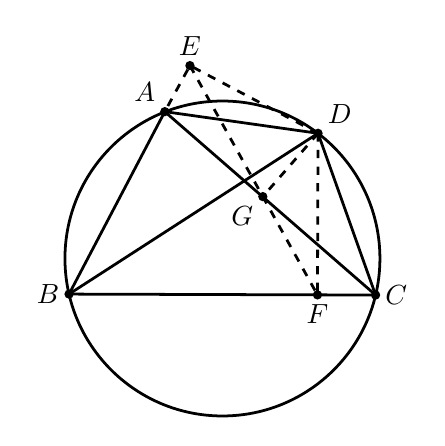
\begin{tikzpicture}[scale=1.0]
\coordinate[] (O) at (0,0);
\coordinate[label=above left:$A$] (A) at (-0.732,1.865);
\coordinate[label=left:$B$] (B) at (-1.948,-0.452);
\coordinate[label=right:$C$] (C) at (1.945,-0.464);
\coordinate[label=above right:$D$] (D) at (1.214,1.59);
\coordinate[label=above:$E$] (E) at (-0.413,2.45);
\coordinate[label=below:$F$] (F) at (1.207,-0.462);
\coordinate[label=below left:$G$] (G) at (0.513,0.786);
\draw [line width=1pt] (O) circle (2cm);
\draw [line width=1pt] (A) -- (B) -- (C) -- (D) -- cycle;
\draw [line width=1pt] (A) -- (C);
\draw [line width=1pt] (B) -- (D);
\draw [dashed,line width=1pt] (D) -- (E) -- (A);
\draw [dashed,line width=1pt] (D) -- (F);
\draw [dashed,line width=1pt] (D) -- (G);
\draw [dashed,line width=1pt] (E) -- (G) -- (F);
\foreach \p in {A,B,C,D,E,F,G}
	\fill[fill=black,draw=black,thick] (\p) circle (1.25pt);
\tkzMarkRightAngle[dashed,line width=1pt](D,E,A);
\tkzMarkRightAngle[dashed,line width=1pt](D,G,C);
\tkzMarkRightAngle[dashed,line width=1pt](D,F,C);
\end{tikzpicture}
\end{figure*}

由四边形包含一组相对的直角, 可以得到三个顶点共圆的四边形, 分别是 $BFDE$, $AGDE$, 和 $CDGF$.

在四边形 $BFDE$ 中, $\angle FDE = 180\degree - \angle ABC$, 而 在四边形 $ABCD$ 中, $\angle ADC = 180\degree - \angle ABC$, 于是 $\angle FDE = \angle ADC$. 减去重叠的角度, 有 $\angle ADE = \angle CDF$.

再由$C,D,F,G$共圆知: $\angle CDF = \angle CGF$; 由 $A,G,D,E$ 共圆知: $\angle ADE = \angle AGE$. 所以 $\angle AGE = \angle CGF$. 这说明 $GE$ 和 $GF$ 在一条直线上, 故 $E,F,G$三点共线.

回到托勒密定理, 由正弦定理得:
\begin{align*}
EG &= AD\cdot\sin\angle GDE\\
GF &= CD\cdot\sin\angle GCF\\
EF &= BD\cdot\sin\angle EBF
\end{align*}
设四边形 $ABCD$ 的外接圆半径为 $2R$, 那么
\begin{align*}
\sin\angle GDE &= \sin\angle GAE = \sin\angle BAC = \frac{BC}{2R}\\
\sin\angle GCF &= \frac{AB}{2R}\\
\sin\angle EBF &= \frac{AC}{2R}
\end{align*}
代入前面的三个等式, 并根据 $EF = EG + GF$, 得
\[BD\cdot\frac{AC}{2R} = AD\cdot\frac{BC}{2R} + CD\cdot\frac{AB}{2R} ,\]
即: $BD\cdot AC = AD\cdot BC + AB\cdot CD$ . 


%------------------------------------------------------------------------------%
\newpage
\noindent 托勒密定理的应用

下图中, 证明: $x\sin\beta + y\sin\alpha = z\sin(\alpha+\beta)$ .
\begin{figure*}[htbp]
\centering
\begin{tikzpicture}[scale=1]
\coordinate[] (O) at (0,0);
\coordinate[] (A) at (-1.985,2.25);
\coordinate[] (B) at (-1.429,-2.638);
\coordinate[] (C) at (0.677,-2.923);
\coordinate[] (D) at (2.807,1.06);
\draw [line width=1pt] (O) circle (3cm);
\draw [line width=1pt] (A) to[edge label'=$x$] (B);
\draw [line width=1pt] (A) to[edge label=$z$] (C);
\draw [line width=1pt] (A) to[edge label=$y$] (D);
\foreach \p in {A,B,C,D}
	\fill[fill=black,draw=black,thick] (\p) circle (1.25pt);
\draw pic["$\alpha$",draw,line width=1pt, angle eccentricity=2.0, angle radius=0.6cm] {angle=B--A--C};
\draw pic["$\beta$",draw,line width=1pt, angle eccentricity=2.0, angle radius=0.35cm] {angle=C--A--D};
\end{tikzpicture}
\end{figure*}

证明: 由托勒密定理, 有 $xb + ya = zc$, 设圆半径为 $r$, 由正弦定理得 
\begin{align*}
a &= 2r\sin\alpha \\
b &= 2r\sin\beta \\
c &= 2r\sin(\alpha+\beta)
\end{align*}
立刻得到 $x\sin\beta + y\sin\alpha = z\sin(\alpha+\beta)$ .
\begin{figure*}[htbp]
\centering
\begin{tikzpicture}[scale=1]
\coordinate[] (O) at (0,0);
\coordinate[] (A) at (-1.985,2.25);
\coordinate[] (B) at (-1.429,-2.638);
\coordinate[] (C) at (0.677,-2.923);
\coordinate[] (D) at (2.807,1.06);
\draw [line width=1pt] (O) circle (3cm);
\draw [line width=1pt] (A) to[edge label'=$x$] (B);
\draw [line width=1pt] (A) to[edge label=$z$] (C);
\draw [line width=1pt] (A) to[edge label=$y$] (D);
\draw [line width=1pt] (C) to[edge label'=$a$] (B);
\draw [line width=1pt] (C) to[edge label'=$b$] (D);
\draw [line width=1pt] (B) to[edge label=$c$] (D);
\foreach \p in {A,B,C,D}
	\fill[fill=black,draw=black,thick] (\p) circle (1.25pt);
\draw pic["$\alpha$",draw,line width=1pt, angle eccentricity=2.0, angle radius=0.6cm] {angle=B--A--C};
\draw pic["$\beta$",draw,line width=1pt, angle eccentricity=2.0, angle radius=0.35cm] {angle=C--A--D};
\end{tikzpicture}
\end{figure*}


%------------------------------------------------------------------------------%
\newpage
圆幂, 根轴, 根心, 蒙日定理

圆幂定理: 过一定点 $P$ 作任意直线, 与半径为 $R$ 的圆 $O$ 交于两点$A,B$, 则 $PA$ 与 $PB$ 长度的乘积是定值, 恒为 $|OP^2 - R^2|$, 而 $OP^2 - R^2$ 称为点 $P$ 对于圆 $O$ 的圆幂, 圆内的点的幂为负数,圆外的点的幂为正数,圆上的点的幂为零. 

圆幂定理是对相交弦定理, 切割线定理及割线定理的总结. 

\begin{figure*}[htbp]
\centering
\begin{minipage}[t]{0.4\linewidth}
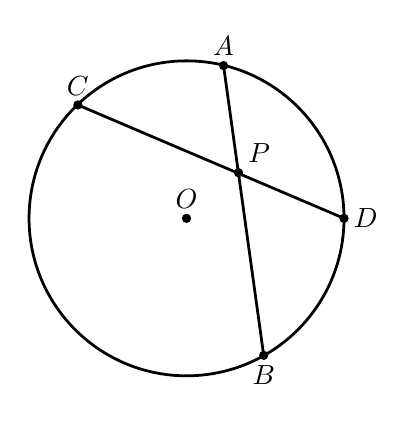
\begin{tikzpicture}[scale=1]
\coordinate[label=$O$] (O) at (0,0);
\coordinate[label=$A$] (A) at (0.47,1.94);
\coordinate[label=$C$] (C) at (-1.38,1.44);
\coordinate[label=below:$B$] (B) at (0.98,-1.74);
\coordinate[label=right:$D$] (D) at (2,0);
\coordinate[label=above right:$P$] (P) at (0.66,0.58);
\coordinate[] (E) at (1.5,1.32);
\coordinate[] (F) at (-1.5,-1.32);
\draw [line width=1pt] (O) circle (2cm);
\draw [line width=1pt] (A) to (B);
\draw [line width=1pt] (C) to (D);
\foreach \p in {O,A,B,C,D,P}
	\fill[fill=black,draw=black,thick] (\p) circle (1.25pt);
\end{tikzpicture}
\end{minipage}
\begin{minipage}[t]{0.4\linewidth}
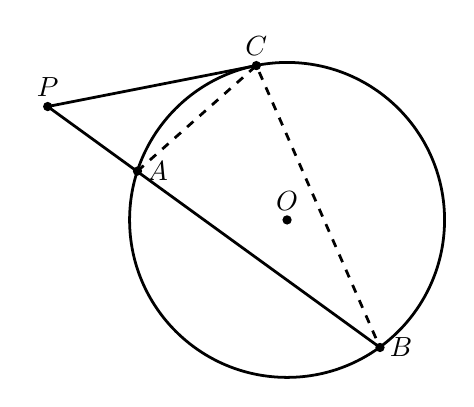
\begin{tikzpicture}[scale=1]
\coordinate[label=$O$] (O) at (0,0);
\coordinate[label=$C$] (C) at (-0.39,1.96);
\coordinate[label=$P$] (P) at (-3.04,1.44);
\coordinate[label=right:$A$] (A) at (-1.9,0.62);
\coordinate[label=right:$B$] (B) at (1.18,-1.62);
\draw [line width=1pt] (O) circle (2cm);
\draw [line width=1pt] (P) to (C);
\draw [line width=1pt] (P) to (B);
\draw [dashed,line width=1pt] (A) -- (C) -- (B);
\foreach \p in {O,A,B,C,P}
	\fill[fill=black,draw=black,thick] (\p) circle (1.25pt);
\end{tikzpicture}
\end{minipage}
\end{figure*}

相交弦定理: 过圆 $O$ 内一点 $P$ 作圆的两个弦 $AB$ 和 $CD$, 则 $PA\cdot PB = PC\cdot PD = (R-OP)(R+OP)$.

切割线定理: 过圆 $O$ 外一点 $P$ 作圆的切线和割线, 割线交圆于 $A,B$ 两点, 而切线的切点为 $C$, 则 $PC^2=PA\cdot PB$.

割线定理: 过圆 $O$ 外一点 $P$ 作圆的两条割线$AB$和$CD$, 则 $PA\cdot PB = PC\cdot PD$. 它们都等于过$P$点的切线长的平方.

根轴: 到固定两圆的圆幂相等的点组成的直线为这两圆的根轴, 这条根轴垂直于连心线.
\begin{figure*}[htbp]
\centering
\begin{minipage}[t]{0.48\linewidth}
\centering
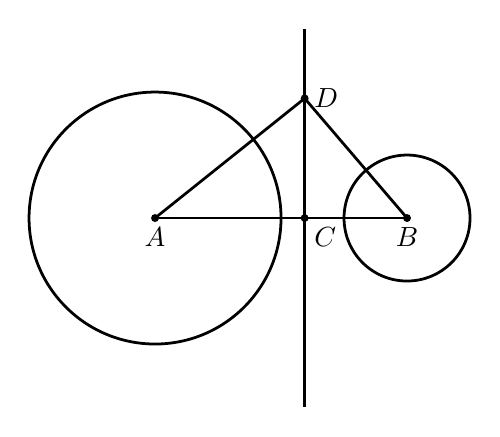
\begin{tikzpicture}[scale=0.8]
\coordinate[label=below:$A$] (A) at (0.0,0.0);
\coordinate[label=below:$B$] (B) at (4.0,0.0);
\coordinate[label=below right:$C$] (C) at (2.375,0);
\coordinate[label=right:$D$] (D) at (2.375,1.9);
\coordinate[] (E) at (2.375,3);
\coordinate[] (F) at (2.375,-3);
\draw [line width=1pt] (A) circle (2cm);
\draw [line width=1pt] (B) circle (1cm);
\draw [line width=1pt] (A) to (B);
\draw [line width=1pt] (E) to (F);
\draw [line width=1pt] (A) -- (D) -- (B);
\foreach \p in {A,B,C,D}
	\fill[fill=black,draw=black,thick] (\p) circle (1.25pt);
\end{tikzpicture}
\end{minipage}
\begin{minipage}[t]{0.48\linewidth}
\centering
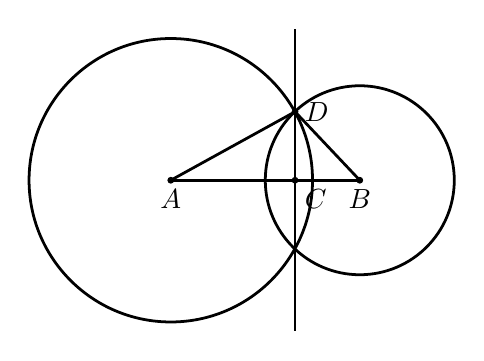
\begin{tikzpicture}[scale=0.6]
\coordinate[label=below:$A$] (A) at (0.0,0.0);
\coordinate[label=below:$B$] (B) at (4.0,0.0);
\coordinate[label=below right:$C$] (C) at (2.63,0);
\coordinate[label=right:$D$] (D) at (2.63,1.45);
\coordinate[] (E) at (2.63,3.2);
\coordinate[] (F) at (2.63,-3.2);
\draw [line width=1pt] (A) circle (3cm);
\draw [line width=1pt] (B) circle (2cm);
\draw [line width=1pt] (A) to (B);
\draw [line width=1pt] (E) to (F);
\draw [line width=1pt] (A) -- (D) -- (B);
\foreach \p in {A,B,C,D}
	\fill[fill=black,draw=black,thick] (\p) circle (1.33pt);
\end{tikzpicture}
\end{minipage}
\end{figure*}

如上图, 两圆 $A,B$ 的半径分别是 $R$ 和 $r$, 连心线 $AB$ 上的点 $C$ 满足 $AC^2-R^2=BC^2-r^2$, $CD \perp AB$. 
当两圆不相交时, 有
\[ AD^2 - R^2 = AC^2+CD^2 - R^2 = BC^2 + CD^2 - r^2 = BD^2 - r^2 .\]
当两圆相交, 根轴是它们的公共弦, 而两圆相切时, 根轴是公切线, 这两种情况下上式也是成立的.
注意只要两圆圆心不重合, 不管位置如何, 根轴总是存在的.

蒙日定理: 三个两两不同心的圆,形成三条根轴,则必有下列三种情况之一:
(1)三根轴两两平行; 
(2)三根轴完全重合;
(3)三根轴两两相交,此时三根轴必汇于一点,该点称为三圆的根心.

证明思路如下: 前两种情况对应三个圆心共线的情形, 当三个圆心不共线时, 假设三个圆心分别是 $A,B,C$, 并且 $A,B$ 的根轴为 $l_1$, $A,C$的根轴为 $l_2$, $l_1$ 与 $l_2$ 相交于点 $P$, 于是 $P$ 点到圆 $A$, 圆 $B$, 圆 $C$ 的圆幂都相等, 说明 $P$ 也位于圆 $A$ 和圆 $C$ 的根轴上.

当两圆 $A,B$ 相离时, 利用根心可以找到它们的根轴. 只要任意作一个圆$C$, 与圆 $A$ 和 $B$ 分别相交, $C$ 不在直线 $AB$ 上, 两个公共弦(或其延长线)相交于点 $P$, 过 $P$ 点作 $AB$ 的垂线就得到了圆 $A$ 和圆 $B$ 的根轴.
\begin{figure*}[htbp]
\centering
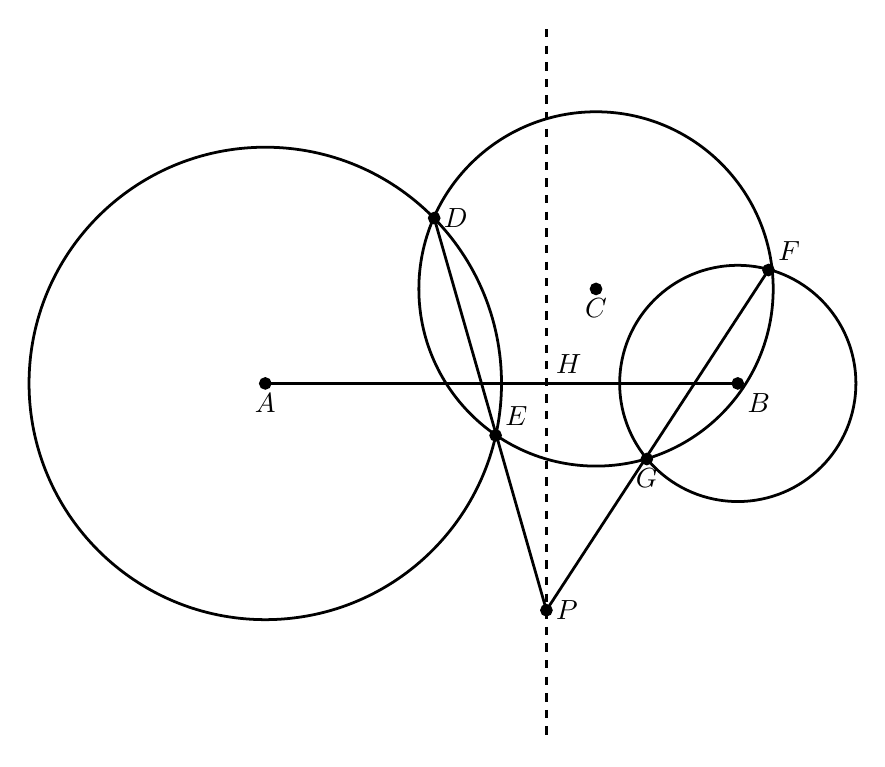
\begin{tikzpicture}[scale=1.5]
\coordinate[label=below:$A$] (A) at (0.0,0.0);
\coordinate[label=below right:$B$] (B) at (4.0,0.0);
\coordinate[label=below:$C$] (C) at (2.8,0.8);
\coordinate[label=right:$D$] (D) at (1.43,1.4);
\coordinate[label=above right:$E$] (E) at (1.95,-0.44);
\coordinate[label=above right:$F$] (F) at (4.26,0.96);
\coordinate[label=below:$G$] (G) at (3.23,-0.64);
\coordinate[label=above right:$H$] (H) at (2.38,0);
\coordinate[] (M) at (2.38,3);
\coordinate[] (N) at (2.38,-3);
\coordinate[label=right:$P$] (P) at (2.38,-1.92);
\draw [line width=1pt] (A) circle (2cm);
\draw [line width=1pt] (B) circle (1cm);
\draw [line width=1pt] (C) circle (1.5cm);
\draw [line width=1pt] (A) to (B);
\draw [line width=1pt] (D) to (P);
\draw [line width=1pt] (F) to (P);
\draw [dashed,line width=1pt] (M) to (N);
\foreach \p in {A,B,C,D,E,F,G,P}
	\fill[fill=black,draw=black,thick] (\p) circle (1.25pt);
\end{tikzpicture}
\end{figure*}

%------------------------------------------------------------------------------%
\newpage

等差幂线: 直线 $AB$ 垂直于 $CD$ 的充要条件是 $AC^2 - AD^2 = BC^2 - BD^2$.
\begin{figure*}[htbp]
\centering
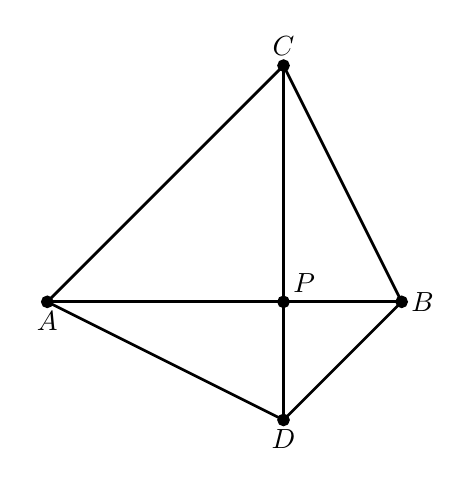
\begin{tikzpicture}[scale=1.5]
\coordinate[label=below:$A$] (A) at (0.0,0.0);
\coordinate[label=right:$B$] (B) at (3.0,0.0);
\coordinate[label=above:$C$] (C) at (2,2);
\coordinate[label=below:$D$] (D) at (2,-1);
\coordinate[label=above right:$P$] (P) at (2,0);
\draw [line width=1pt] (A) to (B);
\draw [line width=1pt] (C) to (D);
\draw [line width=1pt] (A) -- (C) -- (B) -- (D) -- cycle;
\foreach \p in {A,B,C,D,P}
	\fill[fill=black,draw=black,thick] (\p) circle (1.25pt);
\end{tikzpicture}
\end{figure*}

充分性可以由勾股定理直接得到:
\begin{align*}
AC^2 - AD^2 &= (AP^2 + CP^2) - (AP^2 + DP^2) \\
 &=  CP^2 -  DP^2\\
 &= (BP^2 + CP^2) - (BP^2 + DP^2) \\
 &= BC^2 - BD^2.
\end{align*}

必要性, 已知 $AC^2 - AD^2 = BC^2 - BD^2$, 变形为 $AC^2 - BC^2 = AD^2 - BD^2$. 不失一般性, 可以设 $AC > BC$, 过 $B$ 作一个圆, 半径为 $r$, 过 $A$ 作一个圆, 半径为 $R = \sqrt{AC^2 - (BC^2-r^2)}$, 于是 $C$ 到圆 $A$ 的圆幂是 
\[ AC^2 - R^2 = BC^2 - r^2 ,\]
刚好等于$C$ 到圆 $B$ 的圆幂. 
另一方面, 因为$AC^2 - BC^2 = AD^2 - BD^2$, 所以 $R=\sqrt{AD^2 - (BD^2-r^2)}$, 于是
\[ AD^2 - R^2 = BD^2 - r^2 .\]
说明点 $D$ 到圆 $A$ 和 $B$ 的圆幂也是相等的, 所以$CD$是圆 $A$ 和圆 $B$ 的根轴, 从而 $AB$ 垂直于 $CD$.

%------------------------------------------------------------------------------%
\newpage

戴维斯定理: 三角形 $ABC$ 的三边上分别有2点, 依次为 $D,E,F,G,H,I$, 若 $DEFG$ 共圆, $FGHI$共圆, $HIDE$共圆, 则这6点都共圆.
\begin{figure*}[htbp]
\centering
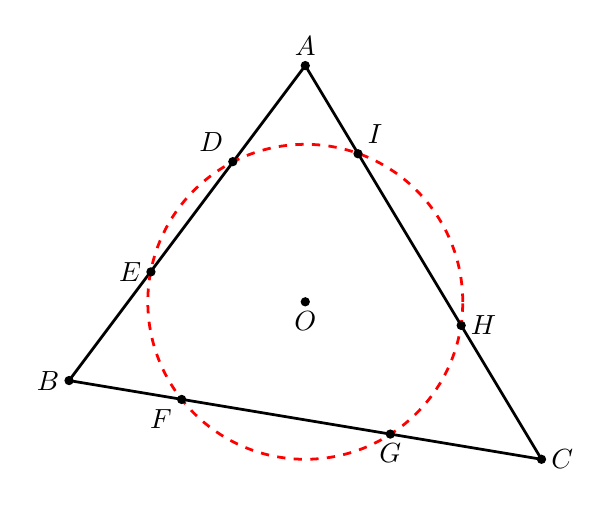
\begin{tikzpicture}[scale=1.0]
\coordinate[label=below:$O$] (O) at (0.0,0.0);
\coordinate[label=above:$A$] (A) at (0.0,3.0);
\coordinate[label=left:$B$] (B) at (-3,-1);
\coordinate[label=right:$C$] (C) at (3,-2);
\coordinate[label=above left:$D$] (D) at (-0.92,1.78);
\coordinate[label=left:$E$] (E) at (-1.96,0.38);
\coordinate[label=below left:$F$] (F) at (-1.57,-1.24);
\coordinate[label=below:$G$] (G) at (1.08,-1.68);
\coordinate[label=right:$H$] (H) at (1.98,-0.3);
\coordinate[label=above right:$I$] (I) at (0.67,1.88);
\draw [line width=1pt] (A) -- (B) -- (C) -- cycle;
\draw [dashed,line width=1pt,red] (O) circle (2cm);
\foreach \p in {A,B,C,D,E,F,G,H,I,O}
	\fill[fill=black,draw=black,thick] (\p) circle (1.25pt);
\end{tikzpicture}
\end{figure*}

(反证) 若6点不共圆, 则点$DEFG$的外接圆与点$FGHI$的外接圆有公共弦 $FG$, 它是这两个圆的根轴. 类似的, 另外两组相交圆对应两条公共弦为 $HI$ 和 $DE$, 这表明三个圆的根轴不交于一点, 与蒙日定理矛盾了.

%------------------------------------------------------------------------------%
\newpage
\section {格点角}
\noindent 来自每日数学打卡

在 $ \triangle ABC $ 中, $ \angle C = 40\degree $, $\angle DAC = 60\degree$, $BD = AC$, 求 $\angle B$ 的度数.

\begin{figure*}[htbp]
\centering
\begin{tikzpicture}[cap=round,scale=1.5]
\tikzstyle{axes}=[line width=1pt]
\coordinate[label=below:$D$] (D) at (0.0,0.0);
\coordinate[label=below:$B$] (B) at (-3.0,0.0);
\coordinate[label=above:$A$] (A) at (0.34,1.93);
\coordinate[label=below:$C$] (C) at (2.64,0.0);
\draw[line width=1pt] (D) to (A);
\draw[line width=1pt] (A) -- (C) -- (B) -- cycle;
\draw pic["$60\degree$", draw, angle eccentricity=1.5] {angle=D--A--C};
\draw pic["$40\degree$", draw, angle eccentricity=1.5] {angle=A--C--D};
\draw pic["?", draw, angle eccentricity=1.5] {angle=D--B--A};
\draw (-1.5, 0) node {$||$} ;
\draw (1.5,0.95) node[rotate=-40] {$||$};
\end{tikzpicture}
\end{figure*}

\noindent 解: 直接建立坐标系. 如下图.
\begin{figure*}[htbp]
\centering
\begin{tikzpicture}[cap=round,scale=1.5]
\tikzstyle{axes}=[line width=1pt]
\coordinate[] (D) at (0.0,0.0);
\coordinate[] (B) at (-3.0,0.0);
\coordinate[] (A) at (0.34,1.93);
\coordinate[] (C) at (2.64,0.0);
\coordinate[] (E) at (0.34,0.0);
\draw[line width=1pt] (B) -- (A) -- (D);

\draw pic["$40\degree$", draw, angle eccentricity=1.5] {angle=A--C--D};
\draw pic["$\alpha$", draw, angle eccentricity=1.5] {angle=D--B--A};
\draw pic["$100\degree$", draw, angle eccentricity=1.5] {angle=A--D--B};
\draw (-1.5, 0) node {$||$} ;
\draw (1.5,0.95) node[rotate=-40] {$||$};
\draw[dashed, line width=1pt] (A) to[edge label=$y$] (E);
\draw[line width=1pt] (D) to[edge label'=$1$] (E);
\draw[line width=1pt] (C) to[edge label=$x$] (E);
\draw[line width=1pt] (A) to[edge node={node [sloped,above] {$\sqrt{x^2+y^2}$}}] (C);
\draw[line width=1pt] (B) to[edge label'=$\sqrt{x^2+y^2}$] (D);
\draw pic["$50\degree$", draw, angle eccentricity=1.5] {angle=E--A--C};
%\draw pic["$80\degree$", draw, angle eccentricity=1.0] {angle=C--D--A};
\tkzMarkRightAngle[line width=1pt](C,E,A);
\end{tikzpicture}
\end{figure*}

 设 $BC$ 为 $x$ 轴, $D$ 为原点, $A$ 的坐标为 $(1,y)$, $CD$ 长是 $1+x$. $CA=BD=\sqrt{x^2+y^2}$, 于是 $\tan 10\degree = \dfrac{1}{y}$, $\tan 50\degree = \dfrac{x}{y}$. 进一步, 
\begin{align*}
\tan\alpha &= \frac{y}{1+\sqrt{x^2+y^2}} = \frac{1}{\frac{1}{y} + \sqrt{1+\frac{x^2}{y^2}}} \\
&= \frac{1}{\tan 10\degree + \sqrt{1+\tan^2 50\degree}} = \frac{1}{\tan 10\degree + \frac{1}{\cos 50\degree}} \\
&= \frac{1}{\frac{\cos 80\degree}{\sin 80\degree} + \frac{1}{\sin 40\degree}} = \frac{\sin 80\degree}{\cos 80\degree + \frac{\sin 80\degree}{\sin 40\degree}} \\
&= \frac{\sin 80\degree}{\cos 80\degree + 2\cos 40\degree} = \frac{\sin 80\degree}{(\cos 80\degree + \cos 40\degree) + \cos 40\degree} \\
&= \frac{\sin 80\degree}{2\cos 60\degree \cos 20\degree + \cos 40\degree} = \frac{\sin 80\degree}{\cos 20\degree + \cos 40\degree}\\
&= \frac{\sin 80\degree}{2\cos 30\degree \cos 10\degree} = \frac{1}{\sqrt{3}}
\end{align*}

于是 $\alpha=30\degree$.

~

\noindent 官方解答1:

由正弦定理: 
\[ \frac{\sin(80\degree - \alpha)}{\sin\alpha} = \frac{BD}{AD} = \frac{AC}{AD} = \frac{\sin 80\degree}{\sin 40\degree} = 2\cos 40\degree = \frac{\cos 40\degree}{\cos 60\degree} = \frac{\sin 50\degree}{\sin 30\degree}.\]
即 $\sin(80\degree - \alpha)\sin 30\degree = \sin 50\degree\sin\alpha$, 由积化和差公式得:
\[ -\frac{1}{2}\left[ \cos(110\degree - \alpha) - \cos(50\degree - \alpha) \right] = -\frac{1}{2}\left[ \cos(50\degree+\alpha) - \cos(50\degree - \alpha)\right].\]
于是 $\cos(110\degree-\alpha) = \cos(50\degree+\alpha)$. 而 $\alpha\in(0,\dfrac{\pi}{2})$, 所以 $110\degree - \alpha = \alpha + 50\degree$.

从而 $\alpha=30\degree$.

~

\noindent 官方解答2:

如下图作辅助线, 以 $AC$ 为边下向作等边三角形 $\triangle ACE$, 连接 $BE$, 在 $BC$ 上截取点 $F$ 使得 $DE = EF$.
\begin{figure*}[htbp]
\centering
\begin{tikzpicture}[cap=round,scale=1.5]
\tikzstyle{axes}=[line width=1pt]
\coordinate[label=below:$D$] (D) at (0.0,0.0);
\coordinate[label=below:$B$] (B) at (-3.0,0.0);
\coordinate[label=above:$A$] (A) at (0.34,1.93);
\coordinate[label=below:$C$] (C) at (2.64,0.0);
\coordinate[label=below:$E$] (E) at (-0.18,-1.03);
\coordinate[label=above:$F$] (F) at (-0.36,0.0);
\draw[line width=1pt] (D) to (A);
\draw[line width=1pt] (A) -- (C) -- (B) -- cycle;
\draw[dashed,line width=1pt] (B) -- (E) -- (C);
\draw[dashed,line width=1pt] (D) -- (E) -- (F);
\draw pic["$60\degree$", draw, angle eccentricity=1.5] {angle=D--A--C};
\draw pic["$40\degree$", draw, angle eccentricity=1.5] {angle=A--C--D};
\draw pic["?", draw, angle eccentricity=1.5] {angle=D--B--A};
\draw (-1.5, 0) node {$||$} ;
\draw (1.5,0.95) node[rotate=-40] {$||$};
\draw (1.22,-0.5) node[rotate=20] {$||$};
\foreach \p in {A,B,C,D,E,F}
	\fill[fill=black,draw=black,thick] (\p) circle (1.25pt);
\end{tikzpicture}
\end{figure*}

所以 $\angle DFE = \angle EDF = 80\degree$, $\angle DEF = 20\degree$.

$\angle CEF= \angle CEA + \angle DEF = 60\degree + 20\degree = 80\degree = \angle CFE$, 所以 $CE=CF$.

又因为 $DE =EF$, $CE=AC=BD$, $\angle CEF = \angle BDE = 80\degree$, 

所以 $\triangle BDE \cong \triangle CEF$. 从而 $BE=CF=CE=BD=AE$, 

由 $BE = AE$, $\angle BEA = 80\degree$ 得 $\angle EBA = 50\degree$, 

再由 $BE=CE$ 得 $\angle EBC = \angle BCE = 20\degree$.

所以 $\angle CBA = \angle EBA - \angle EBC = 30\degree$.


%------------------------------------------------------------------------------%
\newpage
\noindent 来自微博

下图中 $AB=AC$, $\angle PAC = 60\degree$, $\angle PAB = 20\degree$, $\angle PBA = 10\degree$. 求未知角度 $\angle APC$.
\begin{figure*}[htbp]
\centering
\begin{tikzpicture}[scale=1.8]
\coordinate[label=below left:$A$] (A) at (0,0);
\coordinate[label=below right:$C$] (C) at (3,0);
\coordinate[label=above:$B$] (B) at (0.52,2.95);
\coordinate[label=above right:$P$] (P) at (0.52,0.9);
\draw [line width=1pt] (A) -- (B) -- (C) -- cycle;
\draw [line width=1pt] (A) -- (P);
\draw [line width=1pt] (B) -- (P);
\draw [line width=1pt] (C) -- (P);
\foreach \p in {A,B,C,P}
	\fill[fill=black,draw=black,thick] (\p) circle (1.25pt);
\draw pic["$60\degree$",draw,line width=1pt, angle eccentricity=1.6, angle radius=0.5cm] {angle=C--A--P};
\draw pic[draw,line width=1pt, angle eccentricity=2.0, angle radius=0.75cm] {angle=P--A--B};
\draw pic[draw,line width=1pt, angle eccentricity=2.0, angle radius=1.0cm] {angle=A--B--P};
\draw (-0.1,0.4) node[] {$20\degree$};
\draw (0.2,2.4) node[] {$10\degree$};
\draw pic["$?$",draw,line width=1pt, angle eccentricity=1.5, angle radius=0.5cm] {angle=A--P--C};
\draw (1.5,0.0) node[] {$||$};
\draw (0.26,1.47) node[rotate=80] {$||$};
\end{tikzpicture}
\end{figure*}

解: 如下图所示, 以 $AC$ 为边构造等边三角形 $ACD$, 再以 $AP$ 为边构造等边三角形 $AEP$. 连接 $BD$, $DE$, $BE$ 于 $AD$ 的交点为 $F$.
\begin{figure*}[htbp]
\centering
\begin{tikzpicture}[scale=1.8]
\coordinate[label=below left:$A$] (A) at (0,0);
\coordinate[label=below right:$C$] (C) at (3,0);
\coordinate[label=above:$B$] (B) at (0.52,2.95);
\coordinate[label=above:$D$] (D) at (1.5,2.6);
\coordinate[label=below:$E$] (E) at (1.04,0);
\coordinate[label=right:$F$] (F) at (0.8,1.38);
\coordinate[label=above left:$P$] (P) at (0.52,0.9);
\draw [line width=1pt] (A) -- (B) -- (C) -- cycle;
\draw [line width=1pt] (A) -- (P);
\draw [line width=1pt] (B) -- (P);
\draw [line width=1pt] (C) -- (P);
\draw [dashed,line width=1pt] (P) -- (E) -- (B);
\draw [dashed,line width=1pt] (B) -- (D) -- (E);
\draw [dashed,line width=1pt] (C) -- (D) -- (P);
\foreach \p in {A,B,C,D,E,F,P}
	\fill[fill=black,draw=black,thick] (\p) circle (1.25pt);
\draw pic["$60\degree$",draw,line width=1pt, angle eccentricity=1.6, angle radius=0.5cm] {angle=C--A--P};
\draw pic[draw,line width=1pt, angle eccentricity=2.0, angle radius=0.75cm] {angle=P--A--B};
\draw pic[draw,line width=1pt, angle eccentricity=2.0, angle radius=1.0cm] {angle=A--B--P};
\draw (-0.1,0.4) node[] {$20\degree$};
\draw (0.2,2.4) node[] {$10\degree$};
%\draw pic["$?$",draw,line width=1pt, angle eccentricity=1.5, angle radius=0.5cm] {angle=A--P--C};
\draw (1.5,0.0) node[] {$||$};
\draw (0.26,1.47) node[rotate=80] {$||$};
\end{tikzpicture}
\end{figure*}

易知 $BP$ 是 $AE$ 的中垂线. 所以 $\triangle ABE$ 是等腰三角形, 顶角为 $20\degree$. 而由 $AB=AC=AD$, $\triangle ABD$ 也是等腰三角形, 顶角为 $20\degree$, 由 $\angle FAB = \angle FBA$ 得 $AF=BF$, 进而 $DF = EF$, 等腰三角形 $ABF$ 与 $DEF$ 顶角相等, 所以它们相似, 于是 $\angle FAB = \angle FBA = \angle FDE = \angle FED = 20\degree$. (事实上, 由 $\triangle ABE \cong \triangle ABD$, 可以立刻得到四边形 $ABDE$ 为等腰梯形)

又因为 $\triangle ACP \cong \triangle ADE$, 所以 $\angle ACP= \angle ADE = 20\degree$, 于是 $\angle APC = 100\degree$.

%------------------------------------------------------------------------------%
\newpage
\noindent 来自微博:

下图 $\triangle ABC$ 中, $D$ 在 $AC$ 上, $E$ 在 $BC$ 上, $\angle BAC = \angle ABC = \angle ADB = 70\degree$, $CD = BE$, 求 $\angle BDE$.
\begin{figure*}[htbp]
\centering
\begin{tikzpicture}[scale=0.8]
\coordinate[label=below left:$A$] (A) at (0,0);
\coordinate[label=below right:$B$] (B) at (6,0);
\coordinate[label=above:$C$] (C) at (3,8.242);
\coordinate[label=left:$D$] (D) at (1.404,3.857);
\coordinate[label=right:$E$] (E) at (4.404,4.386);
\draw [line width=1pt] (C) --(E) -- (D)-- (A);
\draw [blue,line width=1pt] (D) -- (B)-- (A);
\draw [red,line width=1pt] (B) -- (E)node [midway,sloped] {$\bracevert$};
\draw [red,line width=1pt] (C) -- (D)node [midway,sloped] {$\bracevert$};
\foreach \p in {A,B,C,D,E}
	\fill[fill=black,draw=black,thick] (\p) circle (1.25pt);
\draw pic["$70\degree$",draw,line width=1pt, angle eccentricity=2.0, angle radius=0.35cm] {angle=A--D--B};
\draw pic["$70\degree$",draw,line width=1pt, angle eccentricity=2.0, angle radius=0.35cm] {angle=B--A--D};
\draw pic["$40\degree$",draw,line width=1pt, angle eccentricity=1.8, angle radius=0.55cm] {angle=A--C--B};
\draw pic["$40\degree$",draw,line width=1pt, angle eccentricity=1.8, angle radius=0.55cm] {angle=D--B--A};
\draw pic["$30\degree$",draw,line width=1pt, angle eccentricity=1.8, angle radius=0.65cm] {angle=C--B--D};
\draw pic["$?$",draw,line width=1pt, angle eccentricity=1.6, angle radius=0.5cm] {angle=B--D--E};
\end{tikzpicture}
\end{figure*}

解: 易知 $AB = BD$, $AC = BC$, $AD = AC - CD = BC - BE = EC$. 
作$AD$的中垂线 $BF$, 满足 $BF = AB$, 连接 $DF, EF, AF$. 下面证明 $DFBE$ 四点共圆. 
\begin{figure*}[htbp]
\centering
\begin{tikzpicture}[scale=0.8]
\coordinate[label=below left:$A$] (A) at (0,0);
\coordinate[label=below right:$B$] (B) at (6,0);
\coordinate[label=above:$C$] (C) at (3,8.242);
\coordinate[label=left:$D$] (D) at (1.404,3.857);
\coordinate[label=right:$E$] (E) at (4.404,4.386);
\coordinate[label=left:$F$] (F) at (0.362,2.052);
\coordinate[label=right:$G$] (G) at (7.042,5.909);
\coordinate[] (H) at (3.362,1.523);
\draw [gray,line width=1pt] (H) circle (3.0463cm);
\draw [line width=1pt] (C) --(E) -- (D)-- (A);
\draw [red,line width=1pt] (B) -- (E)node [midway,sloped] {$\bracevert$};
\draw [red,line width=1pt] (C) -- (D)node [midway,sloped] {$\bracevert$};
\draw [blue,line width=1pt] (D) -- (B)-- (A);
\draw [dashed,blue,line width=1pt] (D) -- (G)-- (B) -- (F);
\draw [dashed,red,line width=1pt] (C) -- (G);
\draw [dashed,red,line width=1pt] (E) -- (F);
\draw [dashed,line width=1pt] (D) -- (F) -- (A);
\foreach \p in {A,B,C,D,E,F,G}
	\fill[fill=black,draw=black,thick] (\p) circle (1.25pt);
\draw pic["$40\degree$",draw,line width=1pt, angle eccentricity=1.8, angle radius=0.55cm] {angle=A--C--B};
\draw pic["$40\degree$",draw,line width=1pt, angle eccentricity=1.8, angle radius=0.65cm] {angle=B--C--G};
\draw pic["$50\degree$",draw,line width=1pt, angle eccentricity=1.8, angle radius=0.5cm] {angle=C--G--D};
\draw pic["$30\degree$",draw,line width=1pt, angle eccentricity=1.8, angle radius=0.65cm] {angle=C--B--D};
\draw pic["$30\degree$",draw,line width=1pt, angle eccentricity=1.8, angle radius=0.75cm] {angle=G--B--C};
\draw pic["$20\degree$",draw,line width=1pt, angle eccentricity=1.8, angle radius=1.0cm] {angle=D--B--F};
\draw pic["$20\degree$",draw,line width=1pt, angle eccentricity=1.8, angle radius=0.9cm] {angle=F--B--A};
\end{tikzpicture}
\end{figure*}

作 $D$ 点关于 $BC$ 对称的点 $G$, 连接 $BG, DG, CG$, 则 $\triangle BDG$ 为等边三角形, $BD = DG = BG = BF = AB$, $CD = CG = EB$, $\angle DCG = 80\degree$, $\angle CGD = \angle CDG = 50\degree$.

等腰三角形 $\triangle BDF$ 中, 顶角 $\angle DBF = 20\degree$, $\angle BDF = \angle BFD = 80\degree$. 

由 $\angle EBF = 20\degree + 30\degree = \angle CGD$, $CG = EB$, $DG = FB$ 得 $\triangle CDG \cong \triangle EFB$, 于是 $\angle FEB = \angle DCG = 80\degree = \angle FDB$, 说明 $DFBE$ 四点共圆. 

从而 $\angle BDE = \angle BFE = GDC = 50\degree$.


%------------------------------------------------------------------------------%
\newpage

\noindent 来自微博:

下图中, $AD\perp BC$, $\angle ABE=\angle DBE=10\degree$, $\angle CAD=40\degree$, 求 $\angle BCE$.
\begin{figure*}[htbp]
\centering
\begin{tikzpicture}[scale=1]
\coordinate[label=above:$A$] (A) at (0,3);
\coordinate[label=below left:$B$] (B) at (-8.242, 0);
\coordinate[label=below right:$C$] (C) at (2.517, 0);
\coordinate[label=below:$D$] (D) at (0,0);
\coordinate[label=below left:$E$] (E) at (0, 1.453);
%\coordinate[label=above right:$F$] (F) at (0, 6.916);
%\coordinate[label=above:$G$] (G) at (-2.863, 9.318);
%\coordinate[label=above left:$H$] (H) at (intersection of A--B and E--G);
\draw [line width=1pt] (A) -- (B) --(C) -- (A)-- (D);
\draw [line width=1pt] (B)--(E) --(C);
\foreach \p in {A,B,C,D,E}
	\fill[fill=black,draw=black,thick] (\p) circle (1.25pt);
\tkzMarkRightAngle[line width=1pt](A,D,C);
\draw pic["$40\degree$",draw,line width=1pt, angle eccentricity=1.6, angle radius=0.55cm] {angle=D--A--C};
\draw pic["$10\degree$",draw,line width=1pt, angle eccentricity=1.2, angle radius=2.5cm] {angle=E--B--A};
\draw pic["$10\degree$",draw,line width=1pt, angle eccentricity=1.2, angle radius=2.7cm] {angle=D--B--E};
\draw pic["$?$",draw,line width=1pt, angle eccentricity=1.8, angle radius=0.5cm] {angle=E--C--B};
\end{tikzpicture}
\end{figure*}

解: 延长 $DA$ 至 $F$, 使得 $AF=AC$. 

由 $\angle BAF=180\degree - \angle BAD = 110\degree$, $\angle BAC = \angle BAD + \angle DAC = 110\degree$, 故 $\angle BAF = \angle BAC$, 由 SAS 得 $\triangle BAF\cong \triangle BAC$, 于是 $BF=BC$, $\angle AFB = \angle ACB = 50\degree$.
\begin{figure*}[htbp]
\centering
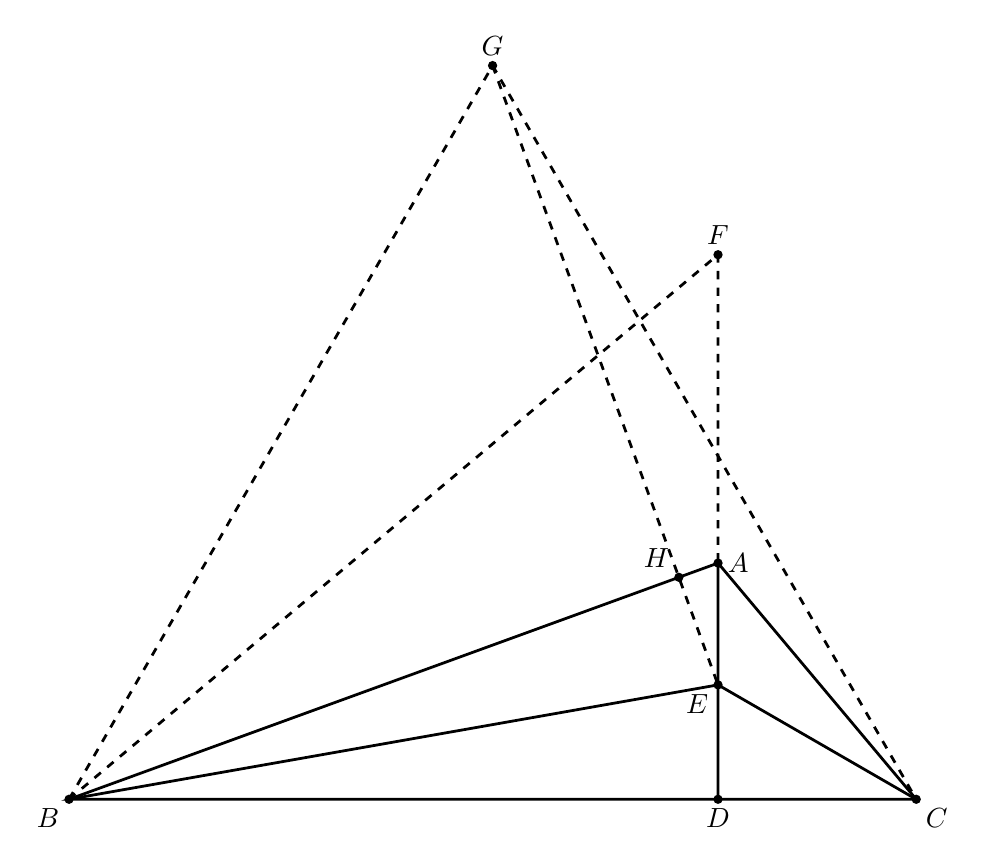
\begin{tikzpicture}[scale=1]
\coordinate[label=right:$A$] (A) at (0,3);
\coordinate[label=below left:$B$] (B) at (-8.242, 0);
\coordinate[label=below right:$C$] (C) at (2.517, 0);
\coordinate[label=below:$D$] (D) at (0,0);
\coordinate[label=below left:$E$] (E) at (0, 1.453);
\coordinate[label=above:$F$] (F) at (0, 6.916);
\coordinate[label=above:$G$] (G) at (-2.863, 9.318);
\coordinate[label=above left:$H$] (H) at (intersection of A--B and E--G);
\draw [line width=1pt] (A) -- (B) --(C) -- (A)-- (D);
\draw [line width=1pt] (B)--(E) --(C);
\draw [dashed,line width=1pt] (B)--(G) --(C);
\draw [dashed,line width=1pt] (G) --(E);
\draw [dashed,line width=1pt] (B)--(F) --(A);
\foreach \p in {A,B,C,D,E,F,G,H}
	\fill[fill=black,draw=black,thick] (\p) circle (1.25pt);
\tkzMarkRightAngle[line width=1pt](A,D,C);
\tkzMarkRightAngle[line width=1pt](B,H,E);
%\draw pic["$40\degree$",draw,line width=1pt, angle eccentricity=1.6, angle radius=0.55cm] {angle=D--A--C};
%\draw pic["$10\degree$",draw,line width=1pt, angle eccentricity=1.2, angle radius=2.5cm] {angle=E--B--A};
%\draw pic["$10\degree$",draw,line width=1pt, angle eccentricity=1.2, angle radius=2.7cm] {angle=D--B--E};
%\draw pic["$?$",draw,line width=1pt, angle eccentricity=1.8, angle radius=0.5cm] {angle=E--C--B};
\end{tikzpicture}
\end{figure*}

作 $EH\perp AB$ 于 $H$, 在直角三角形 $BED$ 和 $BEH$ 中, 由 ASA 得 $\triangle BED \cong \triangle BEH$, 故 $BD = BH$, $\angle BEH = \angle BED = 80\degree$. 

延长$EH$至$G$, 使得$EG=EB$, 则 $\angle BGE = \angle GBE = 50\degree$. $\angle CBG = \angle CBE + \angle EBG = 60\degree$.

在 $\triangle BHG$ 与 $\triangle BDF$ 中, $\angle BHG=\angle BDF=90\degree$, $\angle EGB = \angle DFB = 50\degree$, $BH=BD$, 故 $\triangle BHG\cong \triangle BDF$, $BG=BF$, 推出 $BG=BC$.

由此可得 $\triangle GBC$ 是等边三角形, $\angle BCG = 60\degree$, $BC = GC$. 由 SSS 可得 $\triangle CEG\cong \triangle CEB$, 则 $\angle BCE = \angle GCE = \dfrac{1}{2}BCG = 30\degree$.

~

\noindent 另一种解法

作 $E$ 关于 $AC$ 对称的点 $F$, 以 $BF$ 为边作正三角形 $\triangle BFG$, 并连接 $AG, CF, DF$.
\begin{figure*}[htbp]
\centering
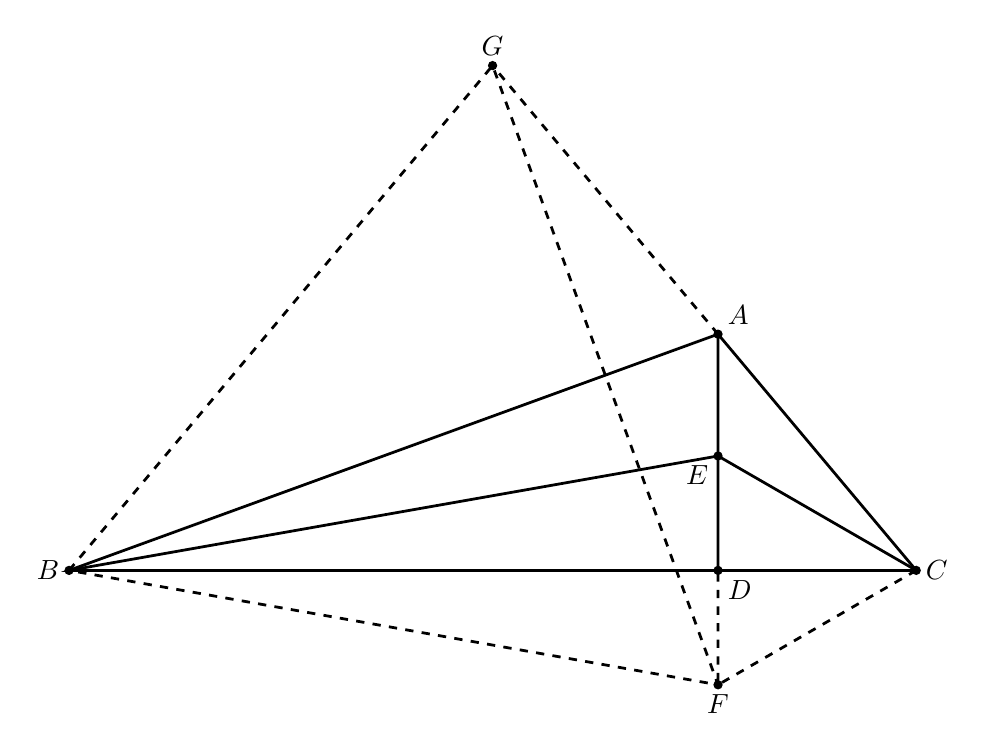
\begin{tikzpicture}[scale=1]
\coordinate[label=above right:$A$] (A) at (0,3);
\coordinate[label=left:$B$] (B) at (-8.242, 0);
\coordinate[label=right:$C$] (C) at (2.517, 0);
\coordinate[label=below right:$D$] (D) at (0,0);
\coordinate[label=below left:$E$] (E) at (0, 1.453);
\coordinate[label=below:$F$] (F) at (0, -1.453);
\coordinate[label=above:$G$] (G) at (-2.863, 6.411);
\draw [line width=1pt] (A) -- (B) --(C) -- (A)-- (D);
\draw [line width=1pt] (B)--(E) --(C);
\draw [dashed,line width=1pt] (B)--(G) --(F)--cycle;
\draw [dashed,line width=1pt] (C)--(F) --(D);
\draw [dashed,line width=1pt] (A)--(G);
\foreach \p in {A,B,C,D,E,F,G}
	\fill[fill=black,draw=black,thick] (\p) circle (1.25pt);
\tkzMarkRightAngle[line width=1pt](A,D,C);
%\draw pic["$40\degree$",draw,line width=1pt, angle eccentricity=1.6, angle radius=0.55cm] {angle=D--A--C};
%\draw pic["$10\degree$",draw,line width=1pt, angle eccentricity=1.2, angle radius=2.5cm] {angle=E--B--A};
%\draw pic["$10\degree$",draw,line width=1pt, angle eccentricity=1.2, angle radius=2.7cm] {angle=D--B--E};
%\draw pic["$?$",draw,line width=1pt, angle eccentricity=1.8, angle radius=0.5cm] {angle=E--C--B};
\end{tikzpicture}
\end{figure*}

$\angle FBC = \angle EBC = 10\degree$, $\angle BFA = 30\degree$, 所以$AB$ 是等边三角形 $\triangle BFG$ 的对称轴, $AB$ 垂直平分 $FG$, 得 $AG = AF$, $\angle AFG = \angle AGF$.

$\angle BFD = \angle BED = 80\degree$, $\angle AFG=\angle AFB - \angle BFG = 20\degree$. 所以 $\angle FAG = 140\degree$, 而 $\angle CAF = 40\degree$, 说明 $G,A,C$ 共线.

$\angle GBC = \angle GBF - \angle FBC = 50\degree$, $\angle ACD = 90\degree- \angle CAD = 50\degree$, 所以 $GC = GC = GF$, 而 $\angle AGF = 20\degree$, 得 $\angle GFC = \angle GCF = 80\degree$, $\angle AFC = \angle GFC - \angle AFG = 60\degree$.

$E,F$ 关于 $BC$ 对称, 所以 $\angle DEC = \angle DFC = 60\degree$, 于是 $\angle BCE = 90\degree-\angle DEC = 30\degree$.

~

用三倍角公式求解: 
\begin{figure*}[htbp]
\centering
\begin{tikzpicture}[scale=1]
\coordinate[label=above:$A$] (A) at (0,3);
\coordinate[label=left:$B$] (B) at (-8.242, 0);
\coordinate[label=right:$C$] (C) at (2.517, 0);
\coordinate[label=below right:$D$] (D) at (0,0);
\coordinate[label=below left:$E$] (E) at (0, 1.453);
\coordinate[label=below:$F$] (F) at (0, -1.453);
\draw [line width=1pt] (A) -- (B) --(C) -- (A)-- (D);
%\draw [line width=1pt] (B)--(E) --(C);
\draw [line width=1pt] (C)--(F) --(D);
\draw [line width=1pt] (B)--(F);
\foreach \p in {A,B,C,D,E,F}
	\fill[fill=black,draw=black,thick] (\p) circle (1.25pt);
\tkzMarkRightAngle[line width=1pt](A,D,C);
\draw pic["$40\degree$",draw,line width=1pt, angle eccentricity=1.8, angle radius=0.5cm] {angle=D--A--C};
\draw pic["$20\degree$",draw,line width=1pt, angle eccentricity=1.5, angle radius=1.2cm] {angle=D--B--A};
\draw pic["$10\degree$",draw,line width=1pt, angle eccentricity=1.5, angle radius=1.8cm] {angle=F--B--D};
\draw pic["$30\degree$",draw,line width=1pt, angle eccentricity=1.8, angle radius=0.6cm] {angle=D--C--F};
\end{tikzpicture}
\end{figure*}

将 $E$ 点沿着 $BC$ 翻折下来, 则 $\angle FBC = 10\degree$, $\angle BCE = \angle BCF$.

可以验证, 正弦和余弦得三倍角分别满足:
\begin{align*}
\sin(3\alpha) &= 4\sin\alpha\sin(60\degree+\alpha)\sin(60\degree-\alpha) \\
\cos(3\alpha) &= 4\cos\alpha\cos(60\degree+\alpha)\cos(60\degree-\alpha)
\end{align*}
于是 
\[\tan(3\alpha) = \tan\alpha\tan(60\degree+\alpha)\tan(60\degree-\alpha) .\]

令 $\alpha=20\degree$, 则 
\begin{align*}
\tan 60\degree &= \tan 20\degree\cdot\tan 80\degree\cdot\tan 40\degree \\
\cot 80\degree &= \cot 60\degree \cdot\tan 20\degree \cdot\tan 40\degree \\
\tan 10\degree &= \tan 20\degree\cdot\tan 30\degree\cdot\tan 40\degree
\end{align*}

回到原题, 
\[\tan 10\degree = \frac{DF}{DB}, \quad \tan 20\degree = \frac{DA}{DB}, \quad \tan 40\degree = \frac{DC}{DA}, \quad \tan\angle DCF = \frac{DF}{DC} .\]
代入得
\[\frac{DF}{DB} = \frac{DA}{DB}\cdot \frac{DC}{DA} \cdot \tan 30\degree .\]
所以
\[\tan 30\degree = \frac{DF}{DC} ,\]
说明 $\angle DCF = 30\degree$.

~

\noindent 推广

基于 $\tan 10\degree = \tan 20\degree\cdot\tan 30\degree\cdot\tan 40\degree$, 可以设计一系列格点角问题. 例如, 可以随意排列四个角度的顺序.
\begin{figure*}[htbp]
\centering
\begin{tikzpicture}[scale=1]
\coordinate[label=above:$A$] (A) at (0,3);
\coordinate[label=left:$B$] (B) at (-8.242, 0);
\coordinate[label=right:$C$] (C) at (1.732, 0);
\coordinate[label=below left:$D$] (D) at (0,0);
\coordinate[label=below left:$E$] (E) at (0, 1.453);
\coordinate[label=below:$F$] (F) at (0, -1.453);
\draw [line width=1pt] (A) -- (B) --(C) -- (A)-- (D);
\draw [dashed,line width=1pt] (B)--(E) --(C);
\draw [line width=1pt] (C)--(F) --(D);
\draw [line width=1pt] (B)--(F);
\foreach \p in {A,B,C,D,E,F}
	\fill[fill=black,draw=black,thick] (\p) circle (1.25pt);
\tkzMarkRightAngle[line width=1pt](A,D,C);
\draw pic["$40\degree$",draw,line width=1pt, angle eccentricity=1.8, angle radius=0.6cm] {angle=D--C--F};
%\draw pic["$20\degree$",draw,line width=1pt, angle eccentricity=1.5, angle radius=1.2cm] {angle=D--B--A};
\draw pic["$10\degree$",draw,line width=1pt, angle eccentricity=1.5, angle radius=1.8cm] {angle=E--B--A};
\draw pic["$10\degree$",draw,line width=1pt, angle eccentricity=1.5, angle radius=1.7cm] {angle=D--B--E};
\draw pic["$10\degree$",draw,line width=1pt, angle eccentricity=1.5, angle radius=1.8cm] {angle=F--B--D};
\draw pic["$30\degree$",draw,line width=1pt, angle eccentricity=1.8, angle radius=0.7cm] {angle=D--A--C};
\end{tikzpicture}
\end{figure*}

若令三倍角公式中的 $\alpha = 10\degree$, 可得 $\tan 30\degree = \tan 10\degree\cdot\tan 70\degree\cdot\tan 50\degree$. 于是可以构造如下的图形.
\begin{figure*}[htbp]
\centering
\begin{tikzpicture}[scale=1]
\coordinate[label=above:$A$] (A) at (0, 3.274);
\coordinate[label=left:$B$] (B) at (-5.671, 0);
\coordinate[label=right:$C$] (C) at (2.747, 0);
\coordinate[label=below left:$D$] (D) at (0,0);
\coordinate[label=below left:$E$] (E) at (0, 1);
\coordinate[label=below:$F$] (F) at (0, -3.274);
\draw [line width=1pt] (A) -- (B) --(C) -- (A)-- (D);
\draw [line width=1pt] (B)--(E) --(C);
\draw [line width=1pt] (C)--(F) --(D);
\draw [line width=1pt] (B)--(F);
\foreach \p in {A,B,C,D,E,F}
	\fill[fill=black,draw=black,thick] (\p) circle (1.25pt);
\tkzMarkRightAngle[line width=1pt](F,D,C);
\draw pic["$50\degree$",draw,line width=1pt, angle eccentricity=1.8, angle radius=0.6cm] {angle=D--C--F};
\draw pic["$70\degree$",draw,line width=1pt, angle eccentricity=1.8, angle radius=0.4cm] {angle=D--E--C};
\draw pic["$20\degree$",draw,line width=1pt, angle eccentricity=1.5, angle radius=1.0cm] {angle=E--B--A};
\draw pic["$10\degree$",draw,line width=1pt, angle eccentricity=1.5, angle radius=1.7cm] {angle=D--B--E};
\draw pic["$30\degree$",draw,line width=1pt, angle eccentricity=1.5, angle radius=0.8cm] {angle=F--B--D};
\draw pic["$40\degree$",draw,line width=1pt, angle eccentricity=1.8, angle radius=0.6cm] {angle=D--A--C};
\end{tikzpicture}
\end{figure*}

此外, 还可以利用关系: $\tan 6\degree = \tan 12\degree\cdot\tan 24\degree\cdot\tan 48\degree$, 构造类似的图. 这个关系不方便直接由三倍角公式得到, 但可以应用两次三倍角公式. 分别令 $\alpha=18\degree$ 和 $\alpha=24\degree$, 根据三倍角公式依次可得:
\begin{align*}
\tan 54\degree &= \tan 18\degree\cdot\tan 78\degree\cdot\tan 42\degree \qquad (1) \\
\tan 72\degree &= \tan 24\degree\cdot\tan 84\degree\cdot\tan 36\degree \qquad (2)
\end{align*}
用 (1) 式除以 (2) 式得:
\[\tan 54\degree\cdot\tan 18\degree = \tan 18\degree\cdot\tan 78\degree\cdot\tan 42\degree\cdot\tan 66\degree\cdot\tan 6\degree\cdot\tan 54\degree .\]
再将含有 $78\degree, 42\degree, 66\degree$ 的项移到左边就得到了
\[\tan 12\degree\cdot\tan 24\degree\cdot\tan48\degree = \tan 6\degree .\]

%------------------------------------------------------------------------------%
\newpage
\noindent 来自微博:

下图中, $AB = CD$, $\angle ABC = 24\degree, \angle BAC = 30\degree$. 求 $\angle ADC$.
\begin{figure*}[htbp]
\centering
\begin{tikzpicture}[scale=1]
\coordinate[label=above:$A$] (A) at (4.517,2.011);
\coordinate[label=below left:$B$] (B) at (0,0);
\coordinate[label=below left:$C$] (C) at (3.056,0);
\coordinate[label=below right:$D$] (D) at (8,0);
%\coordinate[label=below:$E$] (E) at (4,-2.906);
\draw [line width=1pt] (B) --(C) -- (A)-- (D);
\draw [red,line width=1pt] (A) -- (B)node [midway,sloped] {$\bracevert$};
\draw [red,line width=1pt] (C) -- (D)node [midway,sloped] {$\bracevert$};
\foreach \p in {A,B,C,D}
	\fill[fill=black,draw=black,thick] (\p) circle (1.25pt);
\draw pic["$24\degree$",draw,line width=1pt, angle eccentricity=2.2, angle radius=0.55cm] {angle=C--B--A};
\draw pic["$30\degree$",draw,line width=1pt, angle eccentricity=2.0, angle radius=0.5cm] {angle=B--A--C};
\draw pic["$?$",draw,line width=1pt, angle eccentricity=1.8, angle radius=0.5cm] {angle=A--D--C};
\end{tikzpicture}
\end{figure*}

解: 以 $AB$ 为边, $AC$ 为对称轴作等边三角形 $\triangle ABE$, 并在 $BD$ 上截取 $BF = AB$. 连接 $CE, DE, AF, EF$.
\begin{figure*}[htbp]
\centering
\begin{tikzpicture}[scale=1]
\coordinate[label=above:$A$] (A) at (4.517,2.011);
\coordinate[label=below left:$B$] (B) at (0,0);
\coordinate[label=below left:$C$] (C) at (3.056,0);
\coordinate[label=below right:$D$] (D) at (8,0);
\coordinate[label=below:$E$] (E) at (4,-2.906);
\coordinate[label=below right:$F$] (F) at (4.944,0);
\draw [line width=1pt] (B) --(C) -- (A)-- (D);
\draw [red,line width=1pt] (A) -- (B)node [midway,sloped] {$\bracevert$};
\draw [red,line width=1pt] (C) -- (D)node [midway,sloped] {$\bracevert$};
\draw [red,dashed,line width=1pt] (B) -- (E);
\draw [red,dashed,line width=1pt] (A) -- (E);
\draw [blue,dashed,line width=1pt] (C) -- (E) -- (F);
\draw [dashed,line width=1pt] (D) -- (E);
\draw [dashed,line width=1pt] (A) -- (F);
\foreach \p in {A,B,C,D,E,F}
	\fill[fill=black,draw=black,thick] (\p) circle (1.25pt);
\draw pic["$24\degree$",draw,line width=1pt, angle eccentricity=2.2, angle radius=0.6cm] {angle=C--B--A};
\draw pic["$30\degree$",draw,line width=1pt, angle eccentricity=2.0, angle radius=0.5cm] {angle=B--A--C};
\draw pic["$36\degree$",draw,line width=1pt, angle eccentricity=2.0, angle radius=0.5cm] {angle=E--B--C};
\draw pic["$30\degree$",draw,line width=1pt, angle eccentricity=1.8, angle radius=0.65cm] {angle=C--A--E};
\draw pic["$36\degree$",draw,line width=1pt, angle eccentricity=2.0, angle radius=0.5cm] {angle=C--E--B};
\draw pic[draw,line width=1pt, angle eccentricity=2.0, angle radius=0.35cm] {angle=C--F--E};
\draw pic[draw,line width=1pt, angle eccentricity=2.0, angle radius=0.35cm] {angle=E--C--F};
\draw pic["$?$",draw,line width=1pt, angle eccentricity=1.8, angle radius=0.5cm] {angle=A--D--C};
\end{tikzpicture}
\end{figure*}

$\triangle BEF$ 中, $BE = BF$, $\angle EBF = 60\degree - \angle ABC = 36\degree$, $\angle BFE = \angle BEF = 72\degree$. $\angle BEC = \angle CBE = 36\degree, \angle ECF = \angle EBF + \angle BEC = 72\degree = \angle BFE$, 所以 $EC = EF$.

$BF = AB = CD$, 所以 $BC = BF - CF = CD - CF = DF$. 再加上 $\angle BCE = \angle DFE$, 得到 $\triangle BCE\cong\triangle DFE$, 于是 $DE = BE = AE$, 说明 $E$ 是 $\triangle ABD$ 的外心, 所以由圆周角与圆心角的关系得 $\angle ADB = \dfrac{1}{2}\angle AED = 30\degree$.

%------------------------------------------------------------------------------%
\newpage
\noindent 来自微博: 

$\triangle ABC$ 中, $\angle BAC = 80\degree$, $\angle ABC=20\degree$, $D$在$AB$上, $BD=AC$, 求 $\angle ADC$ 的度数.
\begin{figure*}[htbp]
\centering
\begin{tikzpicture}[scale=1]
\coordinate[label=below left:$A$] (A) at (0,0);
\coordinate[label=below right:$B$] (B) at (8,0);
\coordinate[label=above:$C$] (C) at (0.482,2.736);
\coordinate[label=below:$D$] (D) at (5.222,0);
\coordinate[] (E) at (2.611,0.95);
\draw [line width=1pt] (A) --(D) -- (C) -- (B);
\draw [line width=1pt] (C) -- (A) node [midway,sloped] {$||$};
\draw [line width=1pt] (B) -- (D) node [near end,sloped] {$||$};
\foreach \p in {A,B,C,D}
	\fill[fill=black,draw=black,thick] (\p) circle (1.25pt);
\draw pic["$80\degree$",draw,line width=1pt, angle eccentricity=2.5, angle radius=0.3cm] {angle=B--A--C};
\draw pic["$20\degree$",draw,line width=1pt, angle eccentricity=2.3, angle radius=0.6cm] {angle=C--B--A};
\draw pic["$?$",draw,line width=1pt, angle eccentricity=1.5, angle radius=0.6cm] {angle=C--D--A};
\end{tikzpicture}
\end{figure*}

如下图, 以 $AC$ 为边作等边三角形 $ACE$, 并连接 $BE$. 易知 $\triangle ABC$ 是等腰三角形, $BE$为对称轴, $\angle CBE = 10\degree$.
\begin{figure*}[htbp]
\centering
\begin{tikzpicture}[scale=1]
\coordinate[label=below left:$A$] (A) at (0,0);
\coordinate[label=below right:$B$] (B) at (8,0);
\coordinate[label=above:$C$] (C) at (0.482,2.736);
\coordinate[label=below:$D$] (D) at (5.222,0);
\coordinate[label=below right:$E$] (E) at (2.611,0.95);
\draw [line width=1pt] (A) --(D) -- (C) -- (B);
\draw [line width=1pt] (C) -- (A) node [midway,sloped] {$||$};
\draw [line width=1pt] (B) -- (D) node [near end,sloped] {$||$};
\draw [dashed,line width=1pt] (A) --(E) -- (C);
\draw [dashed,line width=1pt] (B) --(E);
\foreach \p in {A,B,C,D,E}
	\fill[fill=black,draw=black,thick] (\p) circle (1.25pt);
\draw pic["$80\degree$",draw,line width=1pt, angle eccentricity=2.5, angle radius=0.3cm] {angle=B--A--C};
\draw pic[draw,line width=1pt, angle eccentricity=2.3, angle radius=0.6cm] {angle=C--B--A};
\draw pic["$?$",draw,line width=1pt, angle eccentricity=1.5, angle radius=0.6cm] {angle=C--D--A};
\end{tikzpicture}
\end{figure*}

考虑 $\triangle CBE$ 和 $\triangle BCD$. 因为 $BD = AC = CE$, $\angle ECB = 20\degree = \angle DBC$, 公共边 $BC$, 所以 $\triangle CBE \cong \triangle BCD$. 

于是 $\angle BCD = \angle CBE = 10\degree$, $\angle ADC = \angle DCB + \angle DBC = 30\degree$.

%------------------------------------------------------------------------------%
\newpage

\noindent 来自微博

已知 $AB=BC=CD$, $\angle ABC = 36\degree$, $\angle BCD = 24\degree$, 求 $\angle ADC$.
\begin{figure*}[htbp]
\centering
\begin{tikzpicture}[scale=1]
\coordinate[label=below left:$C$] (C) at (0,0);
\coordinate[label=below right:$D$] (D) at (6,0);
\coordinate[label=right:$B$] (B) at(5.481, 2.44);
\coordinate[label=left:$A$] (A) at (-0.388, 3.688);
\draw [red,line width=1pt] (A) -- (B) node [midway,sloped] {$\bracevert$};
\draw [red,line width=1pt] (B) -- (C) node [midway,sloped] {$\bracevert$};
\draw [red,line width=1pt] (C) -- (D) node [midway,sloped] {$\bracevert$};
\draw [line width=1pt] (A) -- (D);
\foreach \p in {A,B,C,D}
	\fill[fill=black,draw=black,thick] (\p) circle (1.2pt);
\draw pic["$36\degree$",draw,line width=1pt, angle eccentricity=2.0, angle radius=0.4cm] {angle=A--B--C};
\draw pic["$24\degree$",draw,line width=1pt, angle eccentricity=2.0, angle radius=0.65cm] {angle=D--C--B};
\draw pic["$?$",draw,line width=1pt, angle eccentricity=2.0, angle radius=0.6cm] {angle=A--D--C};
\end{tikzpicture}
\end{figure*}

解: 过 $A$ 作 $AE // BC$, 与$\angle ACB$ 的角平分线交于 $E$, 连接 $BE, DE$. 如下图.
\begin{figure*}[htbp]
\centering
\begin{tikzpicture}[scale=1]
\coordinate[label=below left:$C$] (C) at (0,0);
\coordinate[label=below right:$D$] (D) at (6,0);
\coordinate[label=right:$B$] (B) at(5.481, 2.44);
\coordinate[label=left:$A$] (A) at (-0.388, 3.688);
\coordinate[label=above:$E$] (E) at (3, 5.196);
\coordinate[label=below right:$F$] (F) at (1.854, 3.211);
\draw [red,line width=1pt] (A) -- (B) node [midway,sloped] {$\bracevert$};
\draw [red,line width=1pt] (B) -- (C) node [midway,sloped] {$\bracevert$};
\draw [red,line width=1pt] (C) -- (D) node [midway,sloped] {$\bracevert$};
\draw [line width=1pt] (A) -- (D);
\draw [blue,dashed,line width=1pt] (C) -- (A) -- (E) -- (B);
\draw [red,dashed,line width=1pt] (C) -- (E) -- (D);
\foreach \p in {A,B,C,D,E,F}
	\fill[fill=black,draw=black,thick] (\p) circle (1.2pt);
\draw pic["$36\degree$",draw,line width=1pt, angle eccentricity=2.0, angle radius=0.4cm] {angle=A--B--C};
\draw pic["$24\degree$",draw,line width=1pt, angle eccentricity=2.0, angle radius=0.65cm] {angle=D--C--B};
\draw pic["$?$",draw,line width=1pt, angle eccentricity=2.0, angle radius=0.6cm] {angle=A--D--C};
\end{tikzpicture}
\end{figure*}

容易得到 $\angle BCE = \angle AEC = \angle ABC = \angle EAB = 36\degree$, 由 $AF = EF$, $CF=BF$, $\angle AFC = \angle EFB$, 可得 $\triangle AFC \cong \triangle EFB$, 从而 $AC = EB$, 即四边形 $ACBE$ 为等腰梯形. 再由 $\angle ACE = \angle AEC = 36\degree$, 得 $AC = AE$.

由等腰梯形 $ACBE$ 对角线相等, 得 $CE = AB = CD$. $\angle ECD = 24\degree + 36\degree = 60\degree$, 所以 $\triangle CDE$ 为等边三角形, 得 $DC = DE$.

这样 $AC = AE, DC = DE, DA = DA$ 得 $\triangle ACD\cong\triangle AED$. 所以 $\angle ADC = \angle ADE = 30\degree$.


%------------------------------------------------------------------------------%
\newpage
\noindent 来自微博: 

已知 $\angle DBA = 48\degree$, $\angle CAB = 24\degree$, $AC=AB=BD$, 求 $\angle BDC$.
\begin{figure*}[htbp]
\centering
\begin{tikzpicture}[scale=1.2]
\coordinate[label=below:$A$] (A) at (1.486,-2.574);
\coordinate[label=right:$B$] (B) at (1.989,2.209);
\coordinate[label=above:$C$] (C) at (0,2);
\coordinate[label=below:$D$] (D) at (-1.902,-0.618);
%\coordinate[label=above left:$E$] (E) at (-2.405,4.165);
%\coordinate[label=below:$F$] (F) at (0,0);
\draw [red,line width=1pt] (C) -- (D);
\draw [blue,line width=1pt] (A) -- (B) node [midway,sloped] {$\bracevert$};
\draw [blue,line width=1pt] (A) -- (C) node [midway,sloped] {$\bracevert$};
\draw [blue,line width=1pt] (B) -- (D) node [midway,sloped] {$\bracevert$};
\foreach \p in {A,B,C,D}
	\fill[fill=black,draw=black,thick] (\p) circle (1.0pt);
\draw pic["$24\degree$",draw,line width=1pt, angle eccentricity=2.0, angle radius=0.8cm] {angle=B--A--C};
\draw pic["$48\degree$",draw,line width=1pt, angle eccentricity=2.0, angle radius=0.4cm] {angle=D--B--A};
\draw pic["$?$",draw,line width=1pt, angle eccentricity=2.0, angle radius=0.8cm] {angle=B--D--C};
\end{tikzpicture}
\end{figure*}

解: 如下图, 以 $BD$ 为边作正三角形 $BDE$, 连接 $AE$, 再在 $AE$ 上截取 $EF=EB$, 并连接 $FB, FC, FD, BC$.
\begin{figure*}[htbp]
\centering
\begin{tikzpicture}[scale=1.2]
\coordinate[label=below:$A$] (A) at (1.486,-2.574);
\coordinate[label=right:$B$] (B) at (1.989,2.209);
\coordinate[label=above:$C$] (C) at (0,2);
\coordinate[label=below:$D$] (D) at (-1.902,-0.618);
\coordinate[label=above left:$E$] (E) at (-2.405,4.165);
\coordinate[label=below:$F$] (F) at (0,0);
\draw [red,line width=1pt] (C) -- (D);
\draw [blue,line width=1pt] (A) -- (B) node [midway,sloped] {$\bracevert$};
\draw [blue,line width=1pt] (A) -- (C) node [midway,sloped] {$\bracevert$};
\draw [blue,line width=1pt] (B) -- (D) node [midway,sloped] {$\bracevert$};
\draw [dashed,blue,line width=1pt] (E) -- (D) node [midway,sloped] {$\bracevert$};
\draw [dashed,blue,line width=1pt] (E) -- (B) node [midway,sloped] {$\bracevert$};
\draw [dashed,blue,line width=1pt] (E) -- (F) node [midway,sloped] {$\bracevert$};
\draw [red,line width=1pt] (C) -- (E);
\draw [dashed,green,line width=1pt] (F) -- (A) ;
\draw [dashed,green,line width=1pt] (F) -- (B);
\draw [dashed,magenta,line width=1pt] (D) -- (F);
\draw [dashed,magenta,line width=1pt] (C) -- (F);
\draw [dashed,magenta,line width=1pt] (B) -- (C);
\foreach \p in {A,B,C,D,E,F}
	\fill[fill=black,draw=black,thick] (\p) circle (1.0pt);
\draw pic["$24\degree$",draw,line width=1pt, angle eccentricity=2.0, angle radius=0.8cm] {angle=B--A--C};
\draw pic["$48\degree$",draw,line width=1pt, angle eccentricity=2.0, angle radius=0.4cm] {angle=D--B--A};
\draw pic["$?$",draw,line width=1pt, angle eccentricity=2.0, angle radius=0.8cm] {angle=B--D--C};
\end{tikzpicture}
\end{figure*}

在等腰三角形 $\triangle ABC$ 中各角度数分别为: $\angle BAC = 24\degree, \angle ACB = \angle ABC = 78\degree$. 所以 $\angle DBC = \angle ABC - \angle ABD = 30\degree$. 这说明 $BC$ 是等边三角形 $\triangle BDE$ 得对称轴, 所以 $\angle BDC = \angle BEC$.

在等腰三角形 $\triangle ABE$ 中,各角度数分别为: $\angle ABE = 48\degree + 60\degree = 108\degree$, $\angle BAE = \angle BEA = 36\degree$. 于是 $\angle CAF = \angle BAE - \angle BAC = 12\degree$, $\angle DEF = \angle DEB - \angle BEA = 24\degree$. 两个等腰三角形 $\triangle ABC$ 与 $\triangle EDF$ 顶角都是 $24\degree$, 且腰相等, 所以它们全等, 于是 $DF = BC$.

在等腰三角形 $\triangle EFB$ 中,各角度数分别为: $\angle BEF = 36\degree$, $\angle EBF = \angle EFB = 72\degree$, $\angle FBA = \angle EBA - \angle EBF = 36\degree = BAE$, 所以 $AF = BF$.

考虑$\triangle DBF$ 和 $\triangle CAF$, $\angle DBF = \angle ABD - \angle ABF = 12\degree$, $\angle CAF = \angle BAE - \angle BAC = 12\degree$, 根据 $\angle DBF = \angle CAF$, $AC = BD$, $AF=BF$, 推出 $\triangle DBF \cong \triangle CAF$. 故 $DF = CF = BC$, 进而得 $\triangle ECF\cong\triangle ECB$, 所以$EC$ 平分 $\angle BEF$.

最终, $\angle BDC = \angle BEC = \dfrac{1}{2}\angle BEA= 18\degree$.


%------------------------------------------------------------------------------%
\newpage
\noindent 来自微博:

已知 $\angle BCD = 48\degree$, $\angle ADC = 96\degree$, $BC = CD = DA$, 求 $\angle ABC$.
\begin{figure*}[htbp]
\centering
\begin{tikzpicture}[scale=1]
\coordinate[label=left:$A$] (A) at (0,0);
\coordinate[label=above left:$B$] (B) at (1.478,2.034);
\coordinate[label=above:$C$] (C) at (5.523,4.973);
\coordinate[label=below right:$D$] (D) at (5,0);
%\coordinate[label=above left:$E$] (E) at (0.955,7.006);
%\coordinate[label=below:$F$] (F) at (-2.391,3.291);
%\coordinate[label=below:$G$] (G) at (0.109,-1.04);
%\coordinate[label=below:$H$] (H) at (2.177,1.257);
\draw [line width=1pt] (A) -- (B);
\draw [red,line width=1pt] (A) -- (D) node [midway,sloped] {$\bracevert$};
\draw [red,line width=1pt] (D) -- (C) node [midway,sloped] {$\bracevert$};
\draw [red,line width=1pt] (B) -- (C) node [midway,sloped] {$\bracevert$};
\foreach \p in {A,B,C,D}
	\fill[fill=black,draw=black,thick] (\p) circle (1.0pt);
\draw pic["$48\degree$",draw,line width=1pt, angle eccentricity=2.0, angle radius=0.4cm] {angle=B--C--D};
\draw pic["$96\degree$",draw,line width=1pt, angle eccentricity=2.0, angle radius=0.3cm] {angle=C--D--A};
\draw pic["$?$",draw,line width=1pt, angle eccentricity=2.0, angle radius=0.2cm] {angle=A--B--C};
\end{tikzpicture}
\end{figure*}

解: 以 $CD$ 为边作正五边形 $DCEFG$, 连接 $FD$, $GC$ 交于 $H$, 连接 $BE$, $BF$, $BH$, $AF$, $AG$.
\begin{figure*}[htbp]
\centering
\begin{tikzpicture}[scale=1]
\coordinate[label=left:$A$] (A) at (0,0);
\coordinate[label=above left:$B$] (B) at (1.478,2.034);
\coordinate[label=right:$C$] (C) at (5.523,4.973);
\coordinate[label=below right:$D$] (D) at (5,0);
\coordinate[label=above left:$E$] (E) at (0.955,7.006);
\coordinate[label=left:$F$] (F) at (-2.391,3.291);
\coordinate[label=below:$G$] (G) at (0.109,-1.04);
\coordinate[label=below:$H$] (H) at (2.177,1.257);
\draw [line width=1pt] (A) -- (B);
\draw [red,line width=1pt] (A) -- (D) node [midway,sloped] {$\bracevert$};
\draw [red,line width=1pt] (D) -- (C) node [midway,sloped] {$\bracevert$};
\draw [red,line width=1pt] (B) -- (C) node [midway,sloped] {$\bracevert$};
\draw [dashed,red,line width=1pt] (C) -- (E) node [midway,sloped] {$\bracevert$};
\draw [dashed,red,line width=1pt] (E) -- (F) node [midway,sloped] {$\bracevert$};
\draw [dashed,red,line width=1pt] (F) -- (G) node [midway,sloped] {$\bracevert$};
\draw [dashed,red,line width=1pt] (G) -- (D) node [midway,sloped] {$\bracevert$};
\draw [dashed,red,line width=1pt] (C) -- (H)node [midway,sloped] {$\bracevert$};
\draw [dashed,red,line width=1pt] (E) -- (B);
\draw [dashed,red,line width=1pt] (F) -- (H)node [midway,sloped] {$\bracevert$};
\draw [dashed,green,line width=1pt] (F) -- (A);
\draw [dashed,green,line width=1pt] (F) -- (B);
\draw [dashed,line width=1pt] (A) -- (G);
\draw [dashed,line width=1pt] (B) -- (H);
\draw [dashed,blue,line width=1pt] (G) -- (H);
\draw [dashed,blue,line width=1pt] (H) -- (D);
\foreach \p in {A,B,C,D,E,F,G,H}
	\fill[fill=black,draw=black,thick] (\p) circle (1.0pt);
\draw pic["$48\degree$",draw,line width=1pt, angle eccentricity=2.0, angle radius=0.4cm] {angle=B--C--D};
\draw pic["$96\degree$",draw,line width=1pt, angle eccentricity=2.0, angle radius=0.3cm] {angle=C--D--A};
\draw pic["$60\degree$",draw,line width=1pt, angle eccentricity=2.0, angle radius=0.35cm] {angle=E--C--B};
\end{tikzpicture}
\end{figure*}

在正五边形中, $CE$平行于$FD$, $EF$ 平行于 $CG$, 所以四边形$CEFH$为棱形, $FH = CH = CE = CD = CB = AD = GD = FG$, $\angle CHF \angle CEF = 108\degree$

易知等腰三角形 $\triangle GDC$ 中, 顶角为 $\angle GDC = 108\degree$, 两底角为 $\angle GCD = \angle CGD = 36\degree$, 所以$\angle BCH = \angle BCD - \angle GCD = 12\degree$, $\angle ADG = \angle GDC - \angle ADC = 12\degree$. 于是两个等腰三角形 $\triangle BCH$ 与 $\triangle ADG$ 顶角相等, 腰也相等, 故它们全等, 从而得到 $BH = AG$, 并且底角 $\angle BHC = \angle AGD = 84\degree$,.

再考虑$\triangle AGF$ 与 $\triangle BHF$. 因为 $\angle AGF = \angle DGF - \angle AGD = 24\degree$. 而 $\angle BHF = \angle CHF - \angle CHB = 24\degree$, 加上 $BH = AG, FH = FG$, 所以 $\triangle AGF \cong \triangle BHF$, 从而 $FA = FB$, 且 $\angle HFB = \angle GFA$, 进而 $\angle AFB = \angle CFD = 36\degree$.

等腰三角形 $\triangle FAB$ 中, 顶角为 $36\degree$, 底角为 $\angle FBA = 72\degree$, 等腰三角形 $\triangle BCE$ 中, $\angle BCE = \angle DCE - \angle BCD = 60\degree$, 所以$\triangle BCE$ 为正三角形, $\angle EBC = \angle BEC = 60\degree$, $BE = CE = EF$. 而在等腰三角形 $\triangle FEB$ 中, 顶角 $\angle FEB = \angle CEF - \angle BEC = 48\degree$, 所以底角为 $\angle FBE = 66\degree$.

综上 $\angle ABC = 360\degree - \angle FBA - \angle FBE - \angle EBC = 162\degree$.

%------------------------------------------------------------------------------%
\newpage
\noindent 来自微博

下图中, $AB = BC = CD = DE = EF$, $\angle ABC = 100\degree, \angle BCD = 140\degree, \angle CDE = 110\degree, \angle DEF = 130\degree$, 求 $\angle EFA$. 
\begin{figure*}[htbp]
\centering
\begin{tikzpicture}[scale=1]
\coordinate[label=below left:$B$] (B) at (0,0);
\coordinate[label=below right:$C$] (C) at (4,0);
\coordinate[label=right:$D$] (D) at (7.064,2.571);
\coordinate[label=above right:$E$] (E) at (5.696,6.33);
\coordinate[label=above:$F$] (F) at (1.937,7.698);
\coordinate[label=left:$A$] (A) at (-0.695,3.939);
\draw [red,line width=1pt] (A) -- (B) node [midway,sloped] {$\bracevert$};
\draw [red,line width=1pt] (B) -- (C) node [midway,sloped] {$\bracevert$}; 
\draw [red,line width=1pt] (C) -- (D) node [midway,sloped] {$\bracevert$}; 
\draw [red,line width=1pt] (D) -- (E) node [midway,sloped] {$\bracevert$};
\draw [red,line width=1pt] (E) -- (F) node [midway,sloped] {$\bracevert$};
\draw [line width=1pt] (F) -- (A);
\foreach \p in {A,B,C,D,E,F}
	\fill[fill=black,draw=black,thick] (\p) circle (1.0pt);
\draw pic["$100\degree$",draw,line width=1pt, angle eccentricity=2.0, angle radius=0.4cm] {angle=C--B--A};
\draw pic["$140\degree$",draw,line width=1pt, angle eccentricity=2.0, angle radius=0.4cm] {angle=D--C--B};
\draw pic["$110\degree$",draw,line width=1pt, angle eccentricity=2.0, angle radius=0.4cm] {angle=E--D--C};
\draw pic["$130\degree$",draw,line width=1pt, angle eccentricity=2.0, angle radius=0.4cm] {angle=F--E--D};
\draw pic["$?$",draw,line width=1pt, angle eccentricity=1.6, angle radius=0.4cm] {angle=A--F--E};
\end{tikzpicture}
\end{figure*}

解法1: 以 $EF$ 为边向内作等边三角形 $\triangle EFP$, 连接 $PA, PB, PC, PD$.
\begin{figure*}[htbp]
\centering
\begin{tikzpicture}[scale=1]
\coordinate[label=left:$A$] (A) at (-0.695,3.939);
\coordinate[label=below left:$B$] (B) at (0,0);
\coordinate[label=below right:$C$] (C) at (4,0);
\coordinate[label=right:$D$] (D) at (7.064,2.571);
\coordinate[label=above right:$E$] (E) at (5.696,6.33);
\coordinate[label=above:$F$] (F) at (1.937,7.698);
\coordinate[label=above:$P$] (P) at (2.632,3.759);
\draw [red,line width=1pt] (A) -- (B) node [midway,sloped] {$\bracevert$};
\draw [red,line width=1pt] (B) -- (C) node [midway,sloped] {$\bracevert$}; 
\draw [red,line width=1pt] (C) -- (D) node [midway,sloped] {$\bracevert$}; 
\draw [red,line width=1pt] (D) -- (E) node [midway,sloped] {$\bracevert$};
\draw [red,line width=1pt] (E) -- (F) node [midway,sloped] {$\bracevert$};
\draw [line width=1pt] (F) -- (A);
\draw [red,dashed,line width=1pt] (F) -- (P)node [midway,sloped] {$\bracevert$};
\draw [red,dashed,line width=1pt] (P) -- (E)node [midway,sloped] {$\bracevert$};
\draw [dashed,line width=1pt] (D) -- (P);
\draw [dashed,line width=1pt] (P) -- (C)node [midway,sloped] {$\bracevert$};
\draw [dashed,line width=1pt] (A) -- (P) -- (B);
\foreach \p in {A,B,C,D,E,F,P}
	\fill[fill=black,draw=black,thick] (\p) circle (1.0pt);
\draw pic["$100\degree$",draw,line width=1pt, angle eccentricity=2.0, angle radius=0.4cm] {angle=C--B--A};
\draw pic["$110\degree$",draw,line width=1pt, angle eccentricity=2.0, angle radius=0.4cm] {angle=E--D--C};
\draw pic["$60\degree$",draw,line width=1pt, angle eccentricity=2.0, angle radius=0.4cm] {angle=F--E--P};
\draw pic["$70\degree$",draw,line width=1pt, angle eccentricity=2.0, angle radius=0.35cm] {angle=P--E--D};
\draw pic[draw,line width=1pt, angle eccentricity=1.6, angle radius=0.4cm] {angle=A--F--E};
\draw pic[draw,line width=1pt, angle eccentricity=1.6, angle radius=0.4cm] {angle=D--C--P};
\draw pic[draw,line width=1pt, angle eccentricity=1.6, angle radius=0.4cm] {angle=P--C--B};
\end{tikzpicture}
\end{figure*}

则 $\angle PEF = 60\degree, \angle PED = 70\degree$, $PE = DE$, 所以 $\angle EPD = \angle EDP = 55\degree$. 而由 $\angle PED + \angle CDE = 180\degree$ 得 $PE$ 平行于 $CD$, 再根据 $PE = CD = DE$ 知四边形$CDEP$为棱形, 于是 $CD = CP = BC$ , $\angle PCD = \angle PED = 70\degree$, $\angle CPD = 55\degree$.

等腰三角形 $\triangle BCP$ 中, $BC = PC$, 顶角 $\angle BCP = \angle BCD - \angle PCD = 70\degree$, 所以底角为 $\angle BPC = \angle CBP = 55\degree$. 

$\angle ABP = \angle ABC - \angle CBP = 45\degree$, $\angle BPF = 360\degree - \angle FPE - \angle EPD - \angle DPC - \angle CPB = 135\degree$. 可见 $\angle BPF + \angle ABP = 180\degree$, 所以 $AB$ 与 $FP$ 平行, 而且相等, 故四边形 $ABPF$ 为平行四边形, $\angle AFP = \angle ABP = 45\degree$, 于是 $\angle EFA = \angle AFP + \angle EFP = 105\degree$.

~

解法2: 延长 $AB, CD, EF$, 构成一个大三角形, 如下图.
\begin{figure*}[htbp]
\centering
\begin{tikzpicture}[scale=1]
\coordinate[label=left:$A$] (A) at (-0.695,3.939);
\coordinate[label=below left:$B$] (B) at (0,0);
\coordinate[label=below right:$C$] (C) at (4,0);
\coordinate[label=right:$D$] (D) at (7.064,2.571);
\coordinate[label=above right:$E$] (E) at (5.696,6.33);
\coordinate[label=above:$F$] (F) at (1.937,7.698);
\coordinate[label=left:$L$] (L) at (-1.538,8.979);
\coordinate[label=right:$M$] (M) at (9.775,4.845);
\coordinate[label=below:$N$] (N) at (0.516,-2.924);
\draw [red,line width=1pt] (A) to[edge label'=$a$] (B);
\draw [red,line width=1pt] (B) to[edge label'=$a$] (C);
\draw [red,line width=1pt] (C) to[edge label'=$a$] (D);
\draw [red,line width=1pt] (D) to[edge label'=$a$] (E);
\draw [red,line width=1pt] (E) to[edge label'=$a$] (F);
\draw [line width=1pt] (F) to[edge label=$z$] (A);
\draw [gray,line width=1pt] (F) to[edge label'=$y$]  (L);
\draw [gray,line width=1pt] (L) to[edge label'=$x$]  (A);
\draw [gray,line width=1pt] (B) to [edge label'=$\dfrac{2a}{\sqrt{3}}\sin 40\degree$](N);
\draw [gray,line width=1pt] (C) to [edge label=$\dfrac{2a}{\sqrt{3}}\sin 80\degree$](N);
\draw [gray,line width=1pt] (D) to [edge label'=$\dfrac{2a}{\sqrt{3}}\sin 50\degree$](M);
\draw [gray,line width=1pt] (M) to [edge label'=$\dfrac{2a}{\sqrt{3}}\sin 70\degree$](E);
\foreach \p in {A,B,C,D,E,F,L,M,N}
	\fill[fill=black,draw=black,thick] (\p) circle (1.0pt);
\draw pic["$100\degree$",draw,line width=1pt, angle eccentricity=2.0, angle radius=0.4cm] {angle=C--B--A};
\draw pic["$140\degree$",draw,line width=1pt, angle eccentricity=2.0, angle radius=0.4cm] {angle=D--C--B};
\draw pic["$110\degree$",draw,line width=1pt, angle eccentricity=2.0, angle radius=0.4cm] {angle=E--D--C};
\draw pic["$130\degree$",draw,line width=1pt, angle eccentricity=2.0, angle radius=0.4cm] {angle=F--E--D};
\draw pic["$60\degree$",draw,line width=1pt, angle eccentricity=2.0, angle radius=0.4cm] {angle=C--N--B};
\draw pic["$60\degree$",draw,line width=1pt, angle eccentricity=2.0, angle radius=0.4cm] {angle=E--M--D};
\draw pic["$?$",draw,line width=1pt, angle eccentricity=1.6, angle radius=0.4cm] {angle=A--F--E};
\end{tikzpicture}
\end{figure*}

可以知道 $\angle BNC = \angle DME = 60\degree$, 所以大三角形为等边三角形. 

由正弦定理, 
\begin{align*}
\frac{BN}{\sin 40\degree} &= \frac{CN}{\sin 80\degree} = \frac{a}{\sin 60\degree}\\
\frac{DM}{\sin 50\degree} &= \frac{EM}{\sin 70\degree} = \frac{a}{\sin 60\degree}
\end{align*}
得到
\begin{align*}
BN &= \frac{2a}{\sqrt{3}}\sin 40\degree, \qquad CN = \frac{2a}{\sqrt{3}}\sin 80\degree\\
DM &= \frac{2a}{\sqrt{3}}\sin 50\degree, \qquad EM = \frac{2a}{\sqrt{3}}\sin 70\degree
\end{align*}
根据大等边三角形得边长, 可以求出 $AL, FL$ 的长度分别为:
\begin{align*}
x = AL &= \frac{2a}{\sqrt{3}}(\sin 80\degree + \sin 50\degree - \sin 40\degree) \\
& = \frac{2a}{\sqrt{3}}(\sin 50\degree + \sin 20\degree) = \frac{4a}{\sqrt{3}}\sin 35\degree\cos 15\degree\\
y = FL &= \frac{2a}{\sqrt{3}}(\sin 80\degree + \sin 50\degree - \sin 70\degree) \\
& = \frac{2a}{\sqrt{3}}(\sin 80\degree - \sin10\degree) = \frac{4a}{\sqrt{3}}\sin 35\degree\cos 45\degree  .
\end{align*}
由余弦定理:
\begin{align*}
z^2 &= AF^2 = x^2+y^2-2xy\cos 60\degree\\
&= \frac{16a^2}{3}\sin^2 35\degree(\cos^2 15\degree+\cos^2 45\degree - \cos 15\degree\cos 45\degree) \\
&= \frac{16a^2}{3}\sin^2 35\degree(\frac{1}{2}(\cos 30\degree + 1) + \frac{1}{2}(\cos 90\degree + 1) - \frac{1}{2}(\cos 60\degree + \cos 30\degree)) \\
&= 4a^2\sin^2 35\degree
\end{align*}
故 $z = 2a\sin 35\degree$. 由正弦定理: $\dfrac{z}{\sin 60\degree} = \dfrac{x}{\sin\angle AFL}$, 所以 
\[
\sin \angle AFL = \frac{x\sin 60\degree}{z} = \frac{2}{\sqrt{3}}\sin 60\degree\cos 15\degree =  \sin 75\degree ,
\]
于是 $\angle AFE = 180\degree - \angle AFL = 105\degree$.

~

解法3: 以 $AF, EF$ 为边作平行四边形 $APEF$, 连接 $BP, DP$. 延长 $BA, EF$, 交于 $Q$.
\begin{figure*}[htbp]
\centering
\begin{tikzpicture}[scale=1]
\coordinate[label=left:$A$] (A) at (-0.695,3.939);
\coordinate[label=below left:$B$] (B) at (0,0);
\coordinate[label=below right:$C$] (C) at (4,0);
\coordinate[label=right:$D$] (D) at (7.064,2.571);
\coordinate[label=above right:$E$] (E) at (5.696,6.33);
\coordinate[label=above:$F$] (F) at (1.937,7.698);
\coordinate[label=above:$P$] (P) at (3.064,2.571);
\coordinate[label=left:$Q$] (Q) at (-1.538,8.979);
\draw [red,line width=1pt] (A) -- (B) node [midway,sloped] {$\bracevert$};
\draw [red,line width=1pt] (B) -- (C) node [midway,sloped] {$\bracevert$};
\draw [red,line width=1pt] (C) -- (D) node [midway,sloped] {$\bracevert$};
\draw [red,line width=1pt] (D) -- (E) node [midway,sloped] {$\bracevert$};
\draw [red,line width=1pt] (E) -- (F) node [midway,sloped] {$\bracevert$};
\draw [line width=1pt] (F) -- (A);
\draw [dashed,line width=1pt] (F) -- (Q) -- (A);
\draw [dashed,line width=1pt] (P) -- (E);
\draw [red,dashed,line width=1pt] (P) -- (A) node [midway,sloped] {$\bracevert$};
\draw [red,dashed,line width=1pt] (P) -- (D);
\draw [red,dashed,line width=1pt] (B) -- (P);
\foreach \p in {A,B,C,D,E,F,P,Q}
	\fill[fill=black,draw=black,thick] (\p) circle (1.0pt);
\draw pic["$100\degree$",draw,line width=1pt, angle eccentricity=2.0, angle radius=0.4cm] {angle=C--B--A};
\draw pic["$140\degree$",draw,line width=1pt, angle eccentricity=2.0, angle radius=0.4cm] {angle=D--C--B};
\draw pic["$110\degree$",draw,line width=1pt, angle eccentricity=2.0, angle radius=0.4cm] {angle=E--D--C};
\draw pic["$130\degree$",draw,line width=1pt, angle eccentricity=2.0, angle radius=0.4cm] {angle=F--E--D};
\draw pic["$?$",draw,line width=1pt, angle eccentricity=1.6, angle radius=0.4cm] {angle=A--F--E};
\draw pic["$60\degree$",draw,line width=1pt, angle eccentricity=2.0, angle radius=0.4cm] {angle=A--Q--F};
\draw pic[draw,line width=1pt, angle eccentricity=2.0, angle radius=0.4cm] {angle=B--A--P};
\end{tikzpicture}
\end{figure*}

考虑五边形$BCDEQ$, 由内角和等于 $540\degree$, 可得 $\angle AQF = 60\degree$, 所以 $\angle BAP = \angle AQF = 60\degree$. 又因为 $AB = EF = AP$, 所以 $\triangle ABP$ 为等边三角形, $PB = AB$, $\angle APB = \angle ABP = 60\degree, \angle PBC = \angle ABC - \angle ABP = 40\degree$.

由 $\angle PBC + \angle BCD = 180\degree$ 可得 $BP$ 平行于 $CD$, 又因为 $BP = AB = CD = BC$, 于是四边形 $BCDP$ 是棱形, 得 $PD = CD$, $\angle BPD = \angle BCD = 140\degree, \angle PDC = \angle PBC = 40\degree$. 

$\triangle PDE$ 中, $PD = CD = DE$, $\angle PDE = \angle CDE - \angle PDC = 70\degree$, 所以底角为 $\angle PED = \angle DPE = 55\degree$, 于是 $\angle PEF = \angle DEF - \angle PED = 75\degree$. 平行四边形 $APEF$中, $\angle AFE = 180\degree - \angle PEF = 105\degree$.

~

解法4: 矢量法, 因为 $\vec{AB}+\vec{BC}+\vec{CD}+\vec{DE}+\vec{EF}+\vec{FA} = \vec{0}$, 并注意到向量 $\vec{AB},\vec{CD},\vec{EF}$ 等长且夹角都是 $120\degree$, 所以 $\vec{AB}+\vec{CD}+\vec{EF} = \vec{0}$, 这意味着 $\vec{BC}+\vec{DE}+\vec{FA} = \vec{0}$, 如下图所示.
\begin{figure*}[htbp]
\centering
\begin{minipage}[t]{0.45\linewidth}
\centering
\begin{tikzpicture}[scale=0.7]
\coordinate[label=below left:$B$] (B) at (0,0);
\coordinate[label=below right:$C$] (C) at (4,0);
\coordinate[label=right:$D$] (D) at (7.064,2.571);
\coordinate[label=above right:$E$] (E) at (5.696,6.33);
\coordinate[label=above:$F$] (F) at (1.937,7.698);
\coordinate[label=left:$A$] (A) at (-0.695,3.939);
\draw [red,line width=1pt] (A) -- (B) node [midway,sloped] {$\bracevert$};
\draw [cyan,line width=1pt] (B) -- (C) node [midway,sloped] {$\bracevert$}; 
\draw [green,line width=1pt] (C) -- (D) node [midway,sloped] {$\bracevert$}; 
\draw [blue,line width=1pt] (D) -- (E) node [midway,sloped] {$\bracevert$};
\draw [magenta,line width=1pt] (E) -- (F) node [midway,sloped] {$\bracevert$};
\draw [line width=1pt] (F) -- (A);
\foreach \p in {A,B,C,D,E,F}
	\fill[fill=black,draw=black,thick] (\p) circle (1.0pt);
\draw pic["$100\degree$",draw,line width=1pt, angle eccentricity=2.0, angle radius=0.4cm] {angle=C--B--A};
\draw pic["$140\degree$",draw,line width=1pt, angle eccentricity=2.0, angle radius=0.4cm] {angle=D--C--B};
\draw pic["$110\degree$",draw,line width=1pt, angle eccentricity=2.0, angle radius=0.4cm] {angle=E--D--C};
\draw pic["$130\degree$",draw,line width=1pt, angle eccentricity=2.0, angle radius=0.4cm] {angle=F--E--D};
\draw pic["$?$",draw,line width=1pt, angle eccentricity=1.6, angle radius=0.4cm] {angle=A--F--E};
\end{tikzpicture}
\end{minipage}
\begin{minipage}[t]{0.45\linewidth}
\centering
\begin{tikzpicture}[scale=0.75,>=stealth]
\coordinate[label=above left:$O$] (O) at (0,0);
\coordinate[label=below:$P$] (P) at (0.695,-3.939);
\coordinate[label=right:$Q$] (Q) at (3.759,-1.368);
\coordinate[label=above:$M$] (M) at (2.632,3.759);
\coordinate[label=right:$N$] (N) at (4,0);
\coordinate[] (NX) at (-4,0);
\coordinate[] (MM) at (-2.632,-3.759);
\draw [->,red,line width=1pt] (O) to[edge label'=$\vec{AB}$] (P);
\draw [->,green,line width=1pt] (P) to[edge label'=$\vec{CD}$] (Q);
\draw [->,magenta,line width=1pt] (Q) to[edge label=$\vec{EF}$] (O);
\draw [->,cyan,line width=1pt] (O) to[edge label=$\vec{BC}$] (N);
\draw [->,blue,line width=1pt] (N) to[edge label'=$\vec{DE}$] (M);
\draw [->,line width=1pt] (M) to[edge label'=$\vec{FA}$] (O);
\draw [dashed,line width=1pt] (NX) -- (O);
\draw [dashed,line width=1pt] (MM) -- (O);
\foreach \p in {P,Q,M,N,O}
	\fill[fill=black,draw=black,thick] (\p) circle (1.0pt);
\draw pic["$70\degree$",draw,line width=1pt, angle eccentricity=2.0, angle radius=0.4cm] {angle=M--N--O};
\draw pic[draw,line width=1pt, angle eccentricity=2.0, angle radius=0.4cm] {angle=MM--O--Q};
%\draw pic["$?$",draw,line width=1pt, angle eccentricity=1.6, angle radius=0.4cm] {angle=A--F--E};
\end{tikzpicture}
\end{minipage}
\end{figure*}

而$\vec{BC}$ 与 $\vec{DE}$ 长度相等, 夹角为 $110\degree$, 于是 $\angle MON = 55\degree$, $\vec{BC}$ 与 $\vec{EF}$ 的夹角为 $160\degree$, 所以 $\angle NOQ = 20\degree$, 所求角度为 $180\degree - 55\degree - 20\degree = 105\degree$.


%------------------------------------------------------------------------------%
\newpage
\noindent 来自微博:

正方形 $ABCD$ 中, $E$ 在 $BC$ 上, $F$ 在 $CD$ 上, $\angle AFD = 67\degree, \angle EAB = 22\degree$, 求 $\angle AEF$.
\begin{figure*}[htbp]
\centering
\begin{tikzpicture}[scale=1]
\coordinate[label=below left:$A$] (A) at (0,0);
\coordinate[label=below right:$B$] (B) at (6,0);
\coordinate[label=above right:$C$] (C) at (6,6);
\coordinate[label=above left:$D$] (D) at (0,6);
\coordinate[label=above:$F$] (F) at (2.547,6);
\coordinate[label=right:$E$] (E) at (6,2.424);
%\coordinate[label=below right:$G$] (G) at (1.788,4.212);
\draw [line width=1pt] (A) -- (B) -- (C) -- (D) -- cycle;
\draw [line width=1pt] (A) -- (E) -- (F) -- cycle;
\foreach \p in {A,B,C,D,E,F}
	\fill[fill=black,draw=black,thick] (\p) circle (1.0pt);
\draw pic["$22\degree$",draw,line width=1pt, angle eccentricity=2.0, angle radius=0.7cm] {angle=B--A--E};
\draw pic["$67\degree$",draw,line width=1pt, angle eccentricity=2.0, angle radius=0.4cm] {angle=D--F--A};
\draw pic["$?$",draw,line width=1pt, angle eccentricity=1.6, angle radius=0.4cm] {angle=F--E--A};
\end{tikzpicture}
\end{figure*}

解: 连接 $BD$, 与$AF$相交于 $G$. 连接 $CG, GE$.
\begin{figure*}[htbp]
\centering
\begin{tikzpicture}[scale=1]
\coordinate[label=below left:$A$] (A) at (0,0);
\coordinate[label=below right:$B$] (B) at (6,0);
\coordinate[label=above right:$C$] (C) at (6,6);
\coordinate[label=above left:$D$] (D) at (0,6);
\coordinate[label=above:$F$] (F) at (2.547,6);
\coordinate[label=right:$E$] (E) at (6,2.424);
\coordinate[label=left:$G$] (G) at (1.788,4.212);
\coordinate[] (L) at (4.273,4.212);
\coordinate[] (M) at (3,1.212);
\draw [gray,line width=1pt] (L) circle (2.485558cm);
\draw [gray,line width=1pt] (M) circle (3.235583cm);
\draw [line width=1pt] (A) -- (B) -- (C) -- (D) -- cycle;
\draw [line width=1pt] (A) -- (E) -- (F) -- cycle;
\draw [dashed,line width=1pt] (B) -- (D);
\draw [dashed,line width=1pt] (C) -- (G) -- (E);
\foreach \p in {A,B,C,D,E,F,G}
	\fill[fill=black,draw=black,thick] (\p) circle (1.0pt);
\draw pic["$22\degree$",draw,line width=1pt, angle eccentricity=2.0, angle radius=0.7cm] {angle=B--A--E};
\draw pic["$67\degree$",draw,line width=1pt, angle eccentricity=2.0, angle radius=0.4cm] {angle=D--F--A};
\draw pic["$23\degree$",draw,line width=1pt, angle eccentricity=2.0, angle radius=0.75cm] {angle=F--A--D};
\end{tikzpicture}
\end{figure*}

$\angle DAF = 90\degree - \angle DFA = 23\degree$, $\angle EAG = 90\degree - \angle DAF - \angle EAB = 45\degree = \angle EBG$, 说明 $ABEG$ 四点共圆, 于是 $\angle AEG = \angle ABD = 45\degree$, 且 $\angle AGE = 180\degree - \angle ABE = 90\degree$. 

从而 $\angle FGE = 90\degree$, 加上 $\angle ECF = 90\degree$, 得 $ECFG$四点共圆, 所以 $\angle GCF = \angle GEF$.

易证 $\triangle DGA \cong \triangle DGC$, 所以 $\angle GCD = \angle GAD = 23\degree$. 所以 $\angle AEF = \angle GEF + \angle AEG = 23\degree + 45\degree = 68\degree$.

%------------------------------------------------------------------------------%
\newpage
\noindent 来自微博:

下图中标出了已知角度, 求未知角度.
\begin{figure*}[htbp]
\centering
\begin{tikzpicture}[scale=1]
\coordinate[label=below left:$A$] (A) at (0,0);
\coordinate[label=below right:$B$] (B) at (8,0);
\coordinate[label=above:$C$] (C) at (5.389,3.111);
\coordinate[label=above right:$D$] (D) at (7.518,2.736);
\coordinate[] (E) at (6.128,2.231);
\draw [line width=1pt] (A) --(D) -- (C) -- (B) -- cycle;
\draw [line width=1pt] (A) -- (C);
\draw [line width=1pt] (B) -- (D);
\foreach \p in {A,B,C,D,E}
	\fill[fill=black,draw=black,thick] (\p) circle (1.25pt);
\draw pic["$100\degree$",draw,line width=1pt, angle eccentricity=2.0, angle radius=0.3cm] {angle=A--C--B};
\draw pic["$20\degree$",draw,line width=1pt, angle eccentricity=2.3, angle radius=0.6cm] {angle=B--A--D};
\draw pic["$10\degree$",draw,line width=1pt, angle eccentricity=2.8, angle radius=0.8cm] {angle=D--A--C};
\draw pic["$40\degree$",draw,line width=1pt, angle eccentricity=2.2, angle radius=0.4cm] {angle=B--C--D};
\draw pic["$?$",draw,line width=1pt, angle eccentricity=2.0, angle radius=0.3cm] {angle=A--D--B};
\end{tikzpicture}
\end{figure*}

容易推出 $\angle ADC = 30 \degree, \angle AEC = 70\degree, \triangle ABC = 50\degree$

令 $F$ 是 $\triangle ABC$ 的外心, 连接 $AF, CF, DF$, 设 $DF$ 与 $BC$交于 $H$, 与$AB$交于 $G$. 
\begin{figure*}[htbp]
\centering
\begin{tikzpicture}[scale=1]
\coordinate[label=below left:$A$] (A) at (0,0);
\coordinate[label=below right:$B$] (B) at (8,0);
\coordinate[label=above:$C$] (C) at (5.389,3.111);
\coordinate[label=above right:$D$] (D) at (7.518,2.736);
\coordinate[label=below:$E$] (E) at (6.128,2.231);
\coordinate[label=right:$F$] (F) at (5.389,-3.111);
\coordinate[label=below right:$G$] (G) at (6.522,0);
\coordinate[label=right:$H$] (H) at (6.969,1.229);
\draw [line width=1pt] (A) --(D) -- (C) -- (B) -- cycle;
\draw [line width=1pt] (A) -- (C);
\draw [line width=1pt] (B) -- (D);
\draw [dashed,line width=1pt] (A) -- (F) -- (C);
\draw [dashed,line width=1pt] (D) -- (F);
\draw [dashed,line width=1pt] (A) -- (H);
\foreach \p in {A,B,C,D,E,F,G,H}
	\fill[fill=black,draw=black,thick] (\p) circle (1.25pt);
\draw pic["$100\degree$",draw,line width=1pt, angle eccentricity=2.0, angle radius=0.3cm] {angle=A--C--B};
\draw pic["$20\degree$",draw,line width=1pt, angle eccentricity=2.3, angle radius=0.6cm] {angle=B--A--D};
\draw pic["$10\degree$",draw,line width=1pt, angle eccentricity=2.8, angle radius=0.8cm] {angle=D--A--C};
\draw pic["$40\degree$",draw,line width=1pt, angle eccentricity=2.2, angle radius=0.4cm] {angle=B--C--D};
\draw pic["$50\degree$",draw,line width=1pt, angle eccentricity=2.3, angle radius=0.35cm] {angle=C--B--A};
\draw pic[draw,line width=1pt, angle eccentricity=2.3, angle radius=0.35cm] {angle=B--E--D};
\draw pic[draw,line width=1pt, angle eccentricity=2.3, angle radius=0.5cm] {angle=C--D--A};
\end{tikzpicture}
\end{figure*}

由圆周角和圆心角的关系得 $\angle AFC = 2\angle ADC = 60\degree$, $\angle DFC = 2\angle DAC=20\degree$, 所以 $\angle AFD = 80\degree$, 进而有 $\angle AFH + \angle ACH = 180\degree$, 说明 $A,F,C,H$ 四点共圆.

易证 $\triangle AFC$ 为等边三角形, $\triangle CFD$ 为等腰三角形, 连接 $AH$.
由$A,F,C,H$ 四点共圆得 $\angle HAC = \angle HFC = 20\degree$. 所以 $\angle HAE = \angle HAC - \angle EAC = 10\degree = \angle HAG$. 而 $\angle CHA = \angle CFA = 60\degree$, 公共边 $AH$, 得到 $\triangle AHE \cong \triangle AHG$, 所以 $HE = HG$, $AE = AG$.

而 $\angle AHF = \angle ACF = 60\degree$, $\angle EDH = \angle AHF - \angle HAE = 50\degree = \angle GBH$, $\angle GHB = \angle EHD$, 所以 $\triangle EHD \cong \triangle GHB$, 于是 $ED = GB$. 再由$AE = AG$ 得 $AB = AD$. 所以 $\angle ADB = 80\degree$.


%------------------------------------------------------------------------------%
\newpage
\noindent 来自微博:

下图中, $\angle ABD = 60\degree, \angle CBD = 20\degree, \angle BAC = 50\degree, \angle CAD = 30\degree$, 求 $\angle BDC$.
\begin{figure*}[htbp]
\centering
\begin{tikzpicture}[scale=1]
\coordinate[label=below left:$A$] (A) at (0,0);
\coordinate[label=above left:$B$] (B) at (0,5);
\coordinate[label=above right:$C$] (C) at (4.924,4.132);
\coordinate[label=below right:$D$] (D) at (6.634,1.17);
%\coordinate[label=above right:$E$] (E) at (1.71,0.302);
\draw [line width=1pt] (A) --(D) -- (C) -- (B) -- cycle;
\draw [line width=1pt] (A) -- (C);
\draw [line width=1pt] (B) -- (D);
\foreach \p in {A,B,C,D}
	\fill[fill=black,draw=black,thick] (\p) circle (1.25pt);
\draw pic["$60\degree$",draw,line width=1pt, angle eccentricity=2.0, angle radius=0.4cm] {angle=A--B--D};
\draw pic["$20\degree$",draw,line width=1pt, angle eccentricity=2.2, angle radius=0.6cm] {angle=D--B--C};
\draw pic["$30\degree$",draw,line width=1pt, angle eccentricity=2.2, angle radius=0.6cm] {angle=D--A--C};
\draw pic["$50\degree$",draw,line width=1pt, angle eccentricity=2.0, angle radius=0.4cm] {angle=C--A--B};
\draw pic["$?$",draw,line width=1pt, angle eccentricity=2.0, angle radius=0.5cm] {angle=C--D--B};
\end{tikzpicture}
\end{figure*}

解: 在 $AD$ 上取一点 $E$, 使得 $\angle DBE = 40\degree$, 连接 $BE, CE$.
\begin{figure*}[htbp]
\centering
\begin{tikzpicture}[scale=1]
\coordinate[label=below left:$A$] (A) at (0,0);
\coordinate[label=above left:$B$] (B) at (0,5);
\coordinate[label=above right:$C$] (C) at (4.924,4.132);
\coordinate[label=below right:$D$] (D) at (6.634,1.17);
\coordinate[label=below:$E$] (E) at (1.71,0.302);
\draw [line width=1pt] (A) --(D) -- (C) -- (B) -- cycle;
\draw [line width=1pt] (A) -- (C);
\draw [line width=1pt] (B) -- (D);
\draw [dashed,line width=1pt] (B) -- (E) -- (C);
\foreach \p in {A,B,C,D,E}
	\fill[fill=black,draw=black,thick] (\p) circle (1.25pt);
\draw pic["$40\degree$",draw,line width=1pt, angle eccentricity=2.0, angle radius=0.5cm] {angle=E--B--D};
\draw pic["$20\degree$",draw,line width=1pt, angle eccentricity=2.2, angle radius=0.6cm] {angle=D--B--C};
\draw pic["$30\degree$",draw,line width=1pt, angle eccentricity=2.0, angle radius=0.5cm] {angle=D--A--C};
\draw pic["$50\degree$",draw,line width=1pt, angle eccentricity=2.0, angle radius=0.4cm] {angle=C--A--B};
\draw pic[draw,line width=1pt, angle eccentricity=2.0, angle radius=0.5cm] {angle=C--D--B};
\end{tikzpicture}
\end{figure*}

如此, $\angle CBE = 60\degree, \angle ABE = 20\degree, \angle AEB = 80\degree = \angle BAE$, 于是 $AB = BE$. 而 $\angle BCA = 180\degree - \angle ABC - \angle BAC = 50\degree = \angle BAC$, 所以 $AB = BC = BE$, 于是 $\triangle BCE$为等边三角形, 得 $\angle BEC = 60\degree$, $AB = BE = BC = CE$.

$\triangle BED$ 中, $\angle BED = 180\degree - \angle AEB = 100\degree, \angle BDE = 180\degree - \angle BED - \angle DBE = 40\degree = \angle DBE$, 所以 $BE = DE = CE$. 而等腰三角形 $\triangle CDE$ 中, 顶角度数为 $\angle CED = 180\degree - \angle BEA - \angle BEC = 40\degree$, 所以底角 $\angle ADC = 70\degree$. $\angle ADB = 180\degree - \angle BAD - \angle ABD = 40\degree$, 所以 $\angle BDC = \angle ADC - \angle ADB = 30\degree$. 

%------------------------------------------------------------------------------%
\newpage
\noindent 来自微博:

下图中, $\angle CAB = 70\degree, \angle DAB = 35\degree, \angle ABC = 30\degree, \angle ABD = 65\degree$, 求 $\angle ADC$.
\begin{figure*}[htbp]
\centering
\begin{tikzpicture}[scale=1]
\coordinate[label=left:$A$] (A) at (0,0);
\coordinate[label=right:$B$] (B) at (6,0);
\coordinate[label=above:$C$] (C) at (1.042,2.863);
\coordinate[label=below:$D$] (D) at (4.523,-3.167);
%\coordinate[label=below:$E$] (E) at (1.042,-2.863);
\draw [line width=1pt] (A) --(D) -- (C) -- (B) -- cycle;
\draw [line width=1pt] (A) -- (C);
\draw [line width=1pt] (B) -- (D);
\foreach \p in {A,B,C,D}
	\fill[fill=black,draw=black,thick] (\p) circle (1.25pt);
\draw pic["$70\degree$",draw,line width=1pt, angle eccentricity=2.0, angle radius=0.4cm] {angle=B--A--C};
\draw pic["$35\degree$",draw,line width=1pt, angle eccentricity=2.0, angle radius=0.45cm] {angle=D--A--B};
\draw pic["$30\degree$",draw,line width=1pt, angle eccentricity=2.0, angle radius=0.5cm] {angle=C--B--A};
\draw pic["$65\degree$",draw,line width=1pt, angle eccentricity=2.0, angle radius=0.4cm] {angle=A--B--D};
\draw pic["$?$",draw,line width=1pt, angle eccentricity=2.0, angle radius=0.5cm] {angle=C--D--A};
\end{tikzpicture}
\end{figure*}

解: 设 $AB$ 与 $CD$ 的交点为 $F$, 并作点 $C$ 关于直线 $AB$ 的对称点 $E$, 连接 $AE$, $BE$, $CE$, $DE$. 立刻得到 $\angle BAE = \angle BAC = 70\degree$, $\angle EAD = \angle EAB - \angle BAD = 35\degree$, $\angle EBA = \angle ABC = 30\degree$, $\angle EBD = \angle ABD - \angle ABE = 35\degree$.
\begin{figure*}[htbp]
\centering
\begin{tikzpicture}[scale=1]
\coordinate[label=left:$A$] (A) at (0,0);
\coordinate[label=right:$B$] (B) at (6,0);
\coordinate[label=above:$C$] (C) at (1.042,2.863);
\coordinate[label=below:$D$] (D) at (4.523,-3.167);
\coordinate[label=below:$E$] (E) at (1.042,-2.863);
\coordinate[label=above right:$F$] (F) at (2.695,0);
\draw [line width=1pt] (A) --(D) -- (C) -- (B) -- cycle;
\draw [line width=1pt] (A) -- (C);
\draw [line width=1pt] (B) -- (D);
\draw [dashed,line width=1pt] (A) -- (E) -- (C);
\draw [dashed,line width=1pt] (B) -- (E) -- (D);
\foreach \p in {A,B,C,D,E,F}
	\fill[fill=black,draw=black,thick] (\p) circle (1.25pt);
\draw pic["$70\degree$",draw,line width=1pt, angle eccentricity=2.0, angle radius=0.4cm] {angle=B--A--C};
\draw pic["$35\degree$",draw,line width=1pt, angle eccentricity=2.0, angle radius=0.5cm] {angle=D--A--B};
\draw pic["$30\degree$",draw,line width=1pt, angle eccentricity=2.0, angle radius=0.55cm] {angle=C--B--A};
\draw pic["$30\degree$",draw,line width=1pt, angle eccentricity=2.0, angle radius=0.45cm] {angle=A--B--E};
\draw pic["$35\degree$",draw,line width=1pt, angle eccentricity=2.0, angle radius=0.55cm] {angle=E--B--D};
\draw pic["$35\degree$",draw,line width=1pt, angle eccentricity=2.0, angle radius=0.55cm] {angle=E--A--D};
\draw pic["$?$",draw,line width=1pt, angle eccentricity=2.0, angle radius=0.5cm] {angle=C--D--A};
\end{tikzpicture}
\end{figure*}

则$\angle CBE = 60\degree$, $BC = BE$, 所以 $\triangle BCE$ 为正三角形, 得 $BC = CE$. 

另一方面, $\angle AEB = \angle ACB = 80\degree = \angle ADB$, 所以 $ABDE$ 四点共圆, 进而得到 $\angle DEB = \angle DAB = 35\degree = DBE$, 故 $DE = DB$, 于是 $\triangle CDE \cong \triangle CDB$, 说明 $CD$ 是 $EB$ 的垂直平分线, $\angle BFD = 90\degree - \angle ABE = 60\degree$. 

所以 $\angle ADC = \angle BFD - \angle BAD = 25\degree$. 

%------------------------------------------------------------------------------%
\newpage
\noindent 来自微博: 

下图中, $\angle ABP = 30\degree, \angle PBC = 40\degree, \angle PCB = 20\degree, \angle ACP = 50\degree$. 求 $\angle PAC$.
\begin{figure*}[htbp]
\begin{minipage}[t]{0.45\linewidth}
\centering
\begin{tikzpicture}[scale=1]
\coordinate[label=above:$A$] (A) at (2,5.495);
\coordinate[label=below left:$B$] (B) at (0,0);
\coordinate[label=below right:$C$] (C) at (4,0);
\coordinate[label=below:$P$] (P) at (1.21,1.015);
%\coordinate[label=below:$D$] (D) at (2.79,1.015);
%\coordinate[label=below:$E$] (E) at (-0.274,1.556);
\draw [line width=1pt] (A) -- (B) -- (C) -- cycle;
\draw [line width=1pt] (A) -- (P) -- (B);
\draw [line width=1pt] (P) -- (C);
\foreach \p in {A,B,C,P}
	\fill[fill=black,draw=black,thick] (\p) circle (1.25pt);
\draw pic["$30\degree$",draw,line width=1pt, angle eccentricity=2.1, angle radius=0.55cm] {angle=P--B--A};
\draw pic["$40\degree$",draw,line width=1pt, angle eccentricity=2.0, angle radius=0.45cm] {angle=C--B--P};
\draw pic["$20\degree$",draw,line width=1pt, angle eccentricity=2.2, angle radius=0.6cm] {angle=P--C--B};
\draw pic["$50\degree$",draw,line width=1pt, angle eccentricity=2.0, angle radius=0.4cm] {angle=A--C--P};
\draw pic["$?$",draw,line width=1pt, angle eccentricity=1.6, angle radius=0.5cm] {angle=P--A--C};
\end{tikzpicture}
\end{minipage}
\begin{minipage}[t]{0.45\linewidth}
\centering
\begin{tikzpicture}[scale=1]
\coordinate[label=above:$A$] (A) at (2,5.495);
\coordinate[label=below left:$B$] (B) at (0,0);
\coordinate[label=below right:$C$] (C) at (4,0);
\coordinate[label=below:$P$] (P) at (1.21,1.015);
\coordinate[label=below:$D$] (D) at (2.79,1.015);
\coordinate[label=left:$E$] (E) at (-0.274,1.556);
\draw [line width=1pt] (A) -- (B) -- (C) -- cycle;
\draw [line width=1pt] (A) -- (P) -- (B);
\draw [line width=1pt] (P) -- (C);
\draw [dashed,line width=1pt] (A) --(D) -- (C);
\draw [dashed,line width=1pt] (P) -- (D);
\draw [dashed,line width=1pt] (B) --(E) -- (P);
\draw [dashed,line width=1pt] (A) -- (E);
\foreach \p in {A,B,C,P,D,E}
	\fill[fill=black,draw=black,thick] (\p) circle (1.25pt);
\draw pic["$30\degree$",draw,line width=1pt, angle eccentricity=2.1, angle radius=0.55cm] {angle=P--B--A};
\draw pic["$40\degree$",draw,line width=1pt, angle eccentricity=2.0, angle radius=0.45cm] {angle=C--B--P};
\draw pic["$20\degree$",draw,line width=1pt, angle eccentricity=2.2, angle radius=0.6cm] {angle=P--C--B};
\draw pic[draw,line width=1pt, angle eccentricity=2.0, angle radius=0.4cm] {angle=A--C--P};
\end{tikzpicture}
\end{minipage}
\end{figure*}

解: 过 $P$ 作 $BC$ 的平行线 $PD$, 满足 $\angle ACD = 30\degree$, 在 $CP$ 的延长线上取一点 $E$, 使得 $PB = PE$. 连接 $AE, BE, AD$.

$\angle PCD = 20\degree = DPC$, 故 $DP = DC$. 容易证明 $P$ 和 $D$ 关于 $BC$ 的中垂线对称, 所以 $BP = CD$.

而 $\angle PCB + \angle ABC = 90\degree$, 所以 $CP\perp AB$, 从而 $\angle BPE = 90\degree - \angle ABP = 60\degree$, 又因为 $PB = PE$, 所以 $\triangle BEP$ 为等边三角形, 故有 $BP = PE = BE = DP = CD$.

由 $\angle ABE = \angle ACD = 30\degree$, $BE = CD$, $AB = AC$, 得到 $\triangle ABE\cong\triangle ACD$, 故 $AD = AE$, $\angle CAD = \angle BAE$.

再由 $\angle ABE = \angle ABP = 30\degree$, $BE = BP$, 公共边 $AB$, 得到 $\triangle ABE \cong \triangle ABP$, 所以 $AP = AE$, $\angle BAE = \angle BAP$.

整理上面的结论有 $AD = AE = AP$, 并令 $x = \angle BAE = \angle BAP = \angle CAD$. 由 $PE = PD, AE = AD, AP = AP$ 得 $\triangle APE \cong \triangle APD$, 所以 $\angle PAD = \angle PAE = 2x$.

$\triangle ABC$ 中, $\angle BAC = 40\degree = \angle PAD + \angle CAD + \angle BAP = 4x$, 解得 $x=10\degree$, 所以 $\angle PAC = \angle PAD + \angle CAD = 3x = 30\degree$.


%------------------------------------------------------------------------------%
\newpage

下图等边 $\triangle ABC$ 中, $\angle DBC = 42\degree, \angle DCB = 54\degree$. 求 $\angle BAD$.
\begin{figure*}[htbp]
\centering
\begin{tikzpicture}[scale=1.0]
\coordinate[label=above:$A$] (A) at (0,5.196);
\coordinate[label=below left:$B$] (B) at (-3,0);
\coordinate[label=below right:$C$] (C) at (3,0);
\coordinate[label=left:$D$] (D) at (0.627,3.266);
\draw [line width=1pt] (A) -- (B) -- (C) -- cycle;
\draw [line width=1pt] (A) -- (D) -- (B);
\draw [line width=1pt] (C) -- (D);
\draw pic["$42\degree$",draw,line width=1pt, angle eccentricity=2.0, angle radius=0.4cm] {angle=C--B--D};
\draw pic["$54\degree$",draw,line width=1pt, angle eccentricity=2.0, angle radius=0.4cm] {angle=D--C--B};
\foreach \p in {A,B,C,D}
	\fill[fill=black,draw=black,thick] (\p) circle (1pt);
\end{tikzpicture}
\end{figure*}

解: 作 $\angle CDE = 54\degree$, $DE$ 交 $BC$ 于 $E$. 作 $OE // AC$ 交 $AB$ 于 $O$. 连接 $OD$. 在 $\angle DEC$ 的平分线上取一点 $F$, 使得 $EF = OE$. 连接 $DF$.
\begin{figure*}[htbp]
\centering
\begin{tikzpicture}[scale=1.0]
\coordinate[label=above:$A$] (A) at (0,5.196);
\coordinate[label=below left:$B$] (B) at (-3,0);
\coordinate[label=below right:$C$] (C) at (3,0);
\coordinate[label=left:$D$] (D) at (0.627,3.266);
\coordinate[label=below:$E$] (E) at (-0.434,0);
\coordinate[label=left:$O$] (O) at (-1.717,2.222);
\coordinate[label=below:$F$] (F) at (1.642, 1.508);
\draw [line width=1pt] (A) -- (B) -- (C) -- cycle;
\draw [line width=1pt] (A) -- (D) -- (B);
\draw [line width=1pt] (C) -- (D);
\draw [red,dashed,line width=1pt] (D) -- (O) -- (E) -- (F) -- (D) -- (E);
\foreach \p in {A,B,C,D,E,F,O}
	\fill[fill=black,draw=black,thick] (\p) circle (1pt);
\end{tikzpicture}
\end{figure*}

由 $OE//AC$ 易知 $\triangle BOE$ 为等边三角形. 而 $\angle BDE = 180\degree - \angle DCB - \angle DBC - \angle CDE = 30\degree$, 所以 $O$ 是 $\triangle BDE$ 的外心. 从而 $OD = OE, \angle DOE = 2\angle DBE = 84\degree$, $\angle DEO = \angle DEB - \angle BEO = 48\degree$.

$\angle DEC = 72\degree$, 所以 $\angle DEF = 36\degree$, $\angle OEF = \angle DEO + \angle DEF = 84\degree = \angle DOE$. 又因为 $OD = OE = EF$, 可知四边形 $OEFD$ 为等腰梯形, 所以 $\angle FDE = \angle DEO = 48\degree$.

又易知 $AO = CE = DE$, $\angle AOD = 2\angle ABD = 36\degree = \angle DEF$, $OD = EF$, 所以 $\triangle AOD \cong \triangle DEF$, 得 $\angle BAD = \angle EDF = 48\degree$.


%------------------------------------------------------------------------------%
\newpage

$\triangle ABC$ 中, $\angle ACD = \alpha, \angle DCB = 30\degree, \angle ABD = 30\degree - \alpha, \angle DBC = 60\degree - \alpha$, 求 $\angle CAD$.
\begin{figure*}[htbp]
\centering
\begin{tikzpicture}[scale=1.0]
\coordinate[label=above:$A$] (A) at (3.358,4.978);
\coordinate[label=below left:$B$] (B) at (0,0);
\coordinate[label=below right:$C$] (C) at (8,0);
\coordinate[label=left:$D$] (D) at (3.059,2.853);
\draw [line width=1pt] (A) -- (B) -- (C) -- cycle;
\draw [line width=1pt] (A) -- (D) -- (B);
\draw [line width=1pt] (C) -- (D);
\draw pic["$60\degree - \alpha$",draw,anchor=west,line width=1pt, angle eccentricity=1.0, angle radius=0.5cm] {angle=C--B--D};
\draw pic["",draw,line width=1pt, angle eccentricity=2.0, angle radius=1.0cm] {angle=D--B--A};
\node [rotate=50,anchor=west] at (1.2,1.3) {$30\degree-\alpha$};
\draw pic["$30\degree$",draw,line width=1pt, angle eccentricity=2.0, angle radius=0.6cm] {angle=D--C--B};
\draw pic["$\alpha$",draw,line width=1pt, angle eccentricity=2.0, angle radius=0.8cm] {angle=A--C--D};
\draw pic["$?$",draw,line width=1pt, angle eccentricity=1.6, angle radius=0.5cm] {angle=D--A--C};

\foreach \p in {A,B,C,D}
	\fill[fill=black,draw=black,thick] (\p) circle (1pt);
\end{tikzpicture}
\end{figure*}

解: 分别作 $\triangle BCD$ 和 $\triangle BCA$ 的外接圆$O, O'$. 再连接 $BO$, $CO$, $DO$, $CO'$, $DO'$, $OO'$, $AO'$, $BO'$. 
\begin{figure*}[htbp]
\centering
\begin{tikzpicture}[scale=1.0]
\coordinate[label=above:$A$] (A) at (3.358,4.978);
\coordinate[label=below left:$B$] (B) at (0,0);
\coordinate[label=below right:$C$] (C) at (8,0);
\coordinate[label=left:$D$] (D) at (3.059,2.853);
\coordinate[label=above right:$O'$] (P) at (4,0.923);
\coordinate[label=below:$O$] (O) at (4,-1.223);
\draw [line width=1pt] (A) -- (B) -- (C) -- cycle;
\draw [line width=1pt] (A) -- (D) -- (B);
\draw [line width=1pt] (C) -- (D);
\draw [red,line width=1pt] (B) -- (O) -- (D);
\draw [green,line width=1pt] (C) -- (P) -- (A);
\draw [blue,line width=1pt] (O) -- (P) -- (D);
\draw [green,line width=1pt] (B) -- (P);
\draw [red,line width=1pt] (C) -- (O);
\foreach \p in {A,B,C,D,O,P}
	\fill[fill=black,draw=black,thick] (\p) circle (1pt);
\end{tikzpicture}
\end{figure*}

由 $\angle BCD = 30\degree$, 得 $\angle BOD = 2\angle BCD = 60\degree$, 所以 $\triangle BOD$ 为等边三角形.

$\angle BO'C = 2\angle BAC = 120\degree + 2\alpha$, $\angle CBO' = \angle BCO' = 30\degree - \alpha$. 可得 $\angle DCO' = \angle BCD - \angle BCO' = \alpha$, 以及 $\angle DBO' = \angle CBD - \angle CBO' = 30\degree$, 进而有 $\angle OBO' = 30\degree$, 以及 $\angle CBO = \angle OBO' - \angle CBO' = \alpha$. 

根据 $\angle DCO' = \alpha = \angle ACD$, 以及 $AO'=CO'$ 得 $\angle CAO' = \angle ACO' = 2\alpha$.

由等边$\triangle BOD$ 及 $\angle DBO'=30\degree$ 得 $BO'$ 垂直平分 $DO$, 于是 $\angle BDO' = \angle BOO'$. 再由 $OO'$ 垂直平分 $BC$ 得 $\angle BDO' = \angle BOO' = 90\degree - \angle CBO = 90\degree - \alpha$. 

$\angle CDO' = \angle BDC - \angle BDO' = (90\degree + \alpha) - (90\degree - \alpha) = 2\alpha = \angle CAO'$. 这样可得 $ACDO'$ 四点共圆. 所以$\angle DAO' = \angle DCO' = \alpha$, $\angle CAD = \angle CAO' + \angle DAO' = 3\alpha$.


%------------------------------------------------------------------------------%
\newpage
下图半圆内, $\angle AGC = \angle EGH$, $\angle EHG = \angle DHB$, $\angle CAG = 70\degree$, $\angle DBH = 65\degree$, 求 $\angle GEH$.
\begin{figure*}[htbp]
\centering
\begin{tikzpicture}[scale=1.2]
\coordinate[label=below:$O$] (O) at (0,0);
\coordinate[label=left:$A$] (A) at (-3,0);
\coordinate[label=right:$B$] (B) at (3,0);
\coordinate[label=above left:$C$] (C) at (-2.298, 1.928);
\coordinate[label=above right:$D$] (D) at (1.928, 2.298);
\coordinate[label=above:$E$] (E) at (0.951, 2.845);
%\coordinate[label=below:$F$] (F) at (0.951, -2.845);
\coordinate[label=below:$G$] (G) at (-0.985, 0);
\coordinate[label=below:$H$] (H) at (1.492, 0);
\draw [line width=1pt] (A) -- (B) arc(0:180:3);
\draw [line width=1pt] (A) -- (C) -- (G) -- (E) -- (H) -- (D) -- (B);
\foreach \p in {A,B,C,D,E,G,H,O}
	\fill[fill=black,draw=black,thick] (\p) circle (1.25pt);
\draw pic[red,draw,line width=1pt, angle eccentricity=2.0, angle radius=0.4cm] {angle=C--G--A};
\draw pic[red,draw,line width=1pt, angle eccentricity=2.0, angle radius=0.4cm] {angle=H--G--E};
\draw pic[blue,draw,line width=1pt, angle eccentricity=2.0, angle radius=0.2cm] {angle=E--H--G};
\draw pic[blue,draw,line width=1pt, angle eccentricity=2.0, angle radius=0.2cm] {angle=B--H--D};
\draw pic[blue,draw,line width=1pt, angle eccentricity=2.0, angle radius=0.3cm] {angle=E--H--G};
\draw pic[blue,draw,line width=1pt, angle eccentricity=2.0, angle radius=0.3cm] {angle=B--H--D};
\draw pic["?",draw,line width=1pt, angle eccentricity=2.0, angle radius=0.3cm] {angle=G--E--H};
\draw pic["$70\degree$",draw,line width=1pt, angle eccentricity=2.0, angle radius=0.3cm] {angle=G--A--C};
\draw pic["$65\degree$",draw,line width=1pt, angle eccentricity=2.0, angle radius=0.3cm] {angle=D--B--H};
\end{tikzpicture}
\end{figure*}

解: 延长 $CG$, $DH$, 交于 $F$. 在 $\triangle EGH$ 与 $\triangle FGH$ 中, 有 $\angle FGH = \angle AGC = \angle EGH$, $\angle FHG = \angle DHB = \angle EHG$, 公共边 $GH$, 所以 $\triangle EGH \cong \triangle FGH$, 于是 $OE = OF$, 说明 $F$ 也在圆上.
\begin{figure*}[htbp]
\centering
\begin{tikzpicture}[scale=1.2]
\coordinate[label=below:$O$] (O) at (0,0);
\coordinate[label=left:$A$] (A) at (-3,0);
\coordinate[label=right:$B$] (B) at (3,0);
\coordinate[label=above left:$C$] (C) at (-2.298, 1.928);
\coordinate[label=above right:$D$] (D) at (1.928, 2.298);
\coordinate[label=above:$E$] (E) at (0.951, 2.845);
\coordinate[label=below:$F$] (F) at (0.951, -2.845);
\coordinate[label=below:$G$] (G) at (-0.985, 0);
\coordinate[label=below:$H$] (H) at (1.492, 0);
\draw [line width=1pt] (A) -- (B) arc(0:180:3);
\draw [line width=1pt] (A) -- (C) -- (G) -- (E) -- (H) -- (D) -- (B);
\draw [gray,dashed,line width=1pt] (G)--(F)--(H);
\draw [gray,dashed,line width=1pt] (C)--(O)--(D);
\foreach \p in {A,B,C,D,E,F,G,H,O}
	\fill[fill=black,draw=black,thick] (\p) circle (1.25pt);
\draw pic[red,draw,line width=1pt, angle eccentricity=2.0, angle radius=0.4cm] {angle=C--G--A};
\draw pic[red,draw,line width=1pt, angle eccentricity=2.0, angle radius=0.4cm] {angle=H--G--E};
\draw pic[blue,draw,line width=1pt, angle eccentricity=2.0, angle radius=0.2cm] {angle=E--H--G};
\draw pic[blue,draw,line width=1pt, angle eccentricity=2.0, angle radius=0.2cm] {angle=B--H--D};
\draw pic[blue,draw,line width=1pt, angle eccentricity=2.0, angle radius=0.3cm] {angle=E--H--G};
\draw pic[blue,draw,line width=1pt, angle eccentricity=2.0, angle radius=0.3cm] {angle=B--H--D};
\draw pic["?",draw,line width=1pt, angle eccentricity=2.0, angle radius=0.3cm] {angle=G--E--H};
\draw pic["$70\degree$",draw,line width=1pt, angle eccentricity=2.0, angle radius=0.3cm] {angle=G--A--C};
\draw pic["$65\degree$",draw,line width=1pt, angle eccentricity=2.0, angle radius=0.3cm] {angle=D--B--H};
\end{tikzpicture}
\end{figure*}

而根据等腰三角形 $AOC$ 和 $BOD$ 易知 $\angle AOC = 40\degree$, $\angle BOD = 50\degree$, 于是 $\angle COD = 90\degree$, 进而 $\angle GEH = \angle GFH = \dfrac{1}{2}\angle COD = 45\degree$.


%------------------------------------------------------------------------------%
\newpage

\noindent 来自网络

下图中有三个正六边形, 有一个未知角度 $\alpha$, 求 $\tan\alpha$.
\begin{figure*}[htbp]
\centering
\begin{tikzpicture}[scale=1]
\tikzmath{
	\x1 = -4; \x2 = -3; \x3=-1; \x4=0; \x5=2; \x6=3; \x7=5; \x8=6;
	\y1 =3.464; \y2 =1.732; \y3=0; \y4=-1.732; \y5=-3.464; } 
\coordinate[] (A) at (\x1,\y3);
\coordinate[] (B) at (\x7,\y2);
\coordinate[] (C) at (\x6,\y4);
\draw [line width=1pt] (\x1,\y3) -- (\x2,\y2) -- (\x3,\y2) -- (\x4,\y3)--(\x3,\y4)--(\x2,\y4)--cycle;
\draw [line width=1pt] (\x3,\y2)--(\x4,\y1)--(\x5,\y1)--(\x6,\y2)--(\x5,\y3)--(\x4,\y3);
\draw [line width=1pt] (\x6,\y2)--(\x7,\y2)--(\x8,\y3)--(\x7,\y4)--(\x6,\y4)--(\x5,\y3);
\draw [red,line width=1pt] (A)--(B)--(C);
\foreach \p in {A,B,C}
	\fill[fill=black,draw=black,thick] (\p) circle (1.25pt);
\draw pic["$\alpha$",red,draw,line width=1pt, angle eccentricity=2.0, angle radius=0.4cm] {angle=A--B--C};
\end{tikzpicture}
\end{figure*}

~

解: 将下方补一个正六边形, 易知 $B,C,D$ 共线, 以及 $D,E,A$ 共线, 且 $\angle CDE = 90\degree$.
\begin{figure*}[htbp]
\centering
\begin{tikzpicture}[scale=1]
\tikzmath{
	\x1 = -4; \x2 = -3; \x3=-1; \x4=0; \x5=2; \x6=3; \x7=5; \x8=6;
	\y1 =3.464; \y2 =1.732; \y3=0; \y4=-1.732; \y5=-3.464; } 
\coordinate[label=left:$A$] (A) at (\x1,\y3);
\coordinate[label=above right:$B$] (B) at (\x7,\y2);
\coordinate[label=below right:$C$] (C) at (\x6,\y4);
\coordinate[label=below right:$D$] (D) at (\x5,\y5);
\coordinate[label=below left:$E$] (E) at (\x3,\y4);
\draw [line width=1pt] (\x1,\y3) -- (\x2,\y2) -- (\x3,\y2) -- (\x4,\y3)--(\x3,\y4)--(\x2,\y4)--cycle;
\draw [line width=1pt] (\x3,\y2)--(\x4,\y1)--(\x5,\y1)--(\x6,\y2)--(\x5,\y3)--(\x4,\y3);
\draw [line width=1pt] (\x6,\y2)--(\x7,\y2)--(\x8,\y3)--(\x7,\y4)--(\x6,\y4)--(\x5,\y3);
\draw [line width=1pt] (\x6,\y4)--(\x5,\y5)--(\x4,\y5)--(\x3,\y4);
\draw [red,line width=1pt] (D)--(A)--(B)--(C);
\foreach \p in {A,B,C,D,E}
	\fill[fill=black,draw=black,thick] (\p) circle (1.25pt);
\draw pic["$\alpha$",red,draw,line width=1pt, angle eccentricity=2.0, angle radius=0.4cm] {angle=A--B--C};
\tkzMarkRightAngle[line width=1pt](A,D,C);
\end{tikzpicture}
\end{figure*}

设正六边形边长为 $1$, 则 $BC = 3$, $AD = 2\sqrt{3}$, 所以 $\tan\alpha = \dfrac{2\sqrt{3}}{3}$.

%------------------------------------------------------------------------------%
\newpage

\section{圆}

康威圆: 任意三角形上, 在每个顶点上将两边延伸出去此顶点对应的那边的长度, 这样得到的六点共圆. 这个圆称为此三角形的康威圆.
\begin{figure*}[htbp]
\centering
\begin{tikzpicture}[scale=1.0]
\coordinate[label=below right:$O$] (O) at (0.204,0.744);
\coordinate[label=right:$A$] (A) at (0,2);
\coordinate[label=below right:$B$] (B) at (-1,0);
\coordinate[label=below left:$C$] (C) at (2,0);
\coordinate[label=above left:$D$] (D) at (-2.121,4.121);
\coordinate[label=above:$E$] (E) at (1.342,4.683);
\coordinate[label=left:$F$] (F) at (-3.828,0);
\coordinate[label=below left:$G$] (G) at (-2.265,-2.53);
\coordinate[label=right:$H$] (H) at (4.236,0);
\coordinate[label=below right:$I$] (I) at (3.581,-1.581);
%\coordinate[label=left:$J$] (J) at (-0.462,1.077);
%\coordinate[label=above right:$K$] (K) at (0.73,1.27);
%\coordinate[label=below right:$L$] (L) at (0.204,0);
\draw [gray,line width=1pt] (O) circle (4.1cm);
\draw [red!80,line width=1pt] (A) -- (B);
\draw [red!80,line width=1pt] (H) --(C) -- (I);
\draw [green!80,line width=1pt] (B) -- (C);
\draw [green!80,line width=1pt] (D) -- (A) -- (E);
\draw [blue!80,line width=1pt] (C) -- (A);
\draw [blue!80,line width=1pt] (F) -- (B) -- (G);
\draw [gray,dashed,line width=1pt] (D) -- (O) -- (E);
\draw [gray,dashed,line width=1pt] (F) -- (O) -- (C);
\draw [gray,dashed,line width=1pt] (O) -- (A);
\foreach \p in {A,B,C,D,E,F,G,H,I,O}
	\fill[fill=black,draw=black,thick] (\p) circle (1.25pt);
\end{tikzpicture}
\end{figure*}

如图所示, 设 $\triangle ABC$ 的内心为 $O$. 考虑$\triangle DAO$ 和 $\triangle EAO$, 因为 $\angle BAO = \angle CAO$, $\angle BAD = \angle CAE$, 所以 $\angle DAO = \angle EAO$, 再由 $DA = EA$, 和公共边 $AO$, 得到 $\triangle DAO \cong \triangle EAO$, 所以 $OD = OE$. 同理可得 $OF = OG, OH = OI$.

再考虑$\triangle CDO$ 和 $\triangle CFO$, 因为 $BC = AD, AC = BF$, 所以 $CD = CF$, 再根据 $\angle DCO = \angle FCO$, 和公共边 $CO$, 可得 $\triangle CDO \cong \triangle CFO$, 所以 $OD = OF$. 同理还有 $ OG = OI, OE = OH$.

这就证明了 $O$ 点到 $D,E,F,G,H,I$ 的距离都是相等的.

%------------------------------------------------------------------------------%
\newpage
\noindent 来自每日数学打卡

两圆 $A,B$ 的半径均为 $R$, 并且有两个交点, 如图所示. 另有两个小圆均与 $A$ 内切而与 $B$ 外切, 且两个小圆也相交. 证明两个小圆的公共弦的延长线一定经过 $AB$ 的中点 $M$.

\begin{figure*}[htbp]
\centering
\begin{tikzpicture}[scale=1.2]
\coordinate[label=left:$M$] (M) at (0,0);
\coordinate[label=above left:$A$] (A) at (0,1);
\coordinate[label=above left:$B$] (B) at (0,-1);
\coordinate[label=above left:$C$] (C) at (-1.13,2.19);
\coordinate[label=left:$D$] (D) at (-1.94,1.34);
\coordinate[] (H) at (-1.92,1.87);
\coordinate[] (Q) at (-1.42,1.38);
\coordinate[] (W) at (-3.73,3.6);
\draw [line width=1pt] (A) circle (2.5cm);
\draw [line width=1pt] (B) circle (2.5cm);
\draw [line width=1pt] (C) circle (0.86cm);
\draw [line width=1pt] (D) circle (0.53cm);
\draw [line width=1pt] (H) -- (M);
\draw [dashed,line width=1pt] (A) to [edge label = $R$] (2,2.5);
\draw [dashed,line width=1pt] (B) to [edge label = $R$] (2,0.5);
\draw [dashed,line width=1pt] (A) to (B);
\foreach \p in {M,A,B,C,D,H,Q}
	\fill[fill=black,draw=black,thick] (\p) circle (1.25pt);
\end{tikzpicture}
\end{figure*}

\noindent 证明: 

以 $M$ 为原点, $BA$ 方向为 $y$ 轴建立坐标系, 以下大写字母表示已知长度, 小写字母表示未知长度或坐标. 设 $AB = 2H$, 则 $A(0,H), B(0,-H)$, 圆 $C$ 是内切于$A$ 且外切于$B$ 的任意一个圆, 坐标为 $(u,v)$, 半径为 $w$, 由圆 $C$ 与 $A,B$ 的相切关系有: 
\[ |CA| = R-w, |CB| = R+w. \]
用坐标表示就是:
\begin{align*}
u^2 + (v-H)^2 &= (R-w)^2 \\
u^2 + (v+H)^2 &= (R+w)^2
\end{align*}
由这两个式子可以得到: $v = \dfrac{Rw}{H}$, 以及 $u^2 = R^2+w^2-v^2-H^2$.

现有两圆 $C_1$, $C_2$ 都内切于 $A$ 且外切于 $B$, 圆心分别是 $(u_1,v_1), (u_2,v_2)$, 半径分别是 $w_1, w_2$, 也要满足上面的关系. 圆 $C_1, C_2$ 的方程分别为:
\begin{align*}
(x-u_1)^2 + (y-v_1)^2 &= w_1^2 \\
(x-u_2)^2 + (y-v_2)^2 &= w_2^2 
\end{align*}
联立上两式得到圆 $C_1, C_2$ 公共弦的方程:
\[ 2(u_1-u_2)x + u_2^2-u_1^2 + 2(v_1-v_2)y + v_2^2-v_1^2=w_2-w_1 .\]
将其中的 $u_1^2, u_2^2$ 分别用 $w_1$ 和 $w_2$ 表示, 可以消去 $v_1^2$ 和 $v_2^2$, 最终得到
\[ (u_1-u_2)x+(v_1-v_2)y=0 .\]
这就说明了任意两个这样的圆 $C_1, C_2$ 的公共弦都是经过$(0,0)$点的.

~

\noindent 官方解答:

\begin{figure*}[htbp]
\centering
\begin{tikzpicture}[scale=1.2]
\coordinate[label=left:$M$] (M) at (0,0);
\coordinate[label=above left:$A$] (A) at (0,1);
\coordinate[label=above left:$B$] (B) at (0,-1);
\coordinate[label=above left:$C$] (C) at (-1.13,2.19);
\coordinate[label=left:$T$] (T) at (-0.73,1.43);
\coordinate[label=above left:$S$] (S) at (-1.52,2.96);
%\coordinate[label=left:$D$] (D) at (-1.94,1.34);
%\coordinate[] (H) at (-1.92,1.87);
%\coordinate[] (Q) at (-1.42,1.38);
%\coordinate[] (W) at (-3.73,3.6);
\draw [line width=1pt] (A) circle (2.5cm);
\draw [line width=1pt] (B) circle (2.5cm);
\draw [line width=1pt] (C) circle (0.86cm);
%\draw [line width=1pt] (D) circle (0.53cm);
%\draw [line width=1pt] (H) -- (M);
%\draw [dashed,line width=1pt] (A) to [edge label = $R$] (2,2.5);
%\draw [dashed,line width=1pt] (B) to [edge label = $R$] (2,0.5);
\draw [dashed,line width=1pt] (A) to (B);
\draw [dashed,line width=1pt] (A) to (C);
\draw [dashed,line width=1pt] (B) to (C);
\draw [dashed,line width=1pt] (M) to (S);
\foreach \p in {M,A,B,C,S,T}
	\fill[fill=black,draw=black,thick] (\p) circle (1.25pt);
\end{tikzpicture}
\end{figure*}

设任意一个内切于$A$且外切于$B$小圆 $C$ 的半径为 $r$, 连接 $MC$, 交圆 $C$ 于 $S,T$ 两点; 并连接 $AC, BC$.

根据圆的相切关系可得: $AC=R-r, BC=R+r$, 又因为 $MC$ 是 $\triangle ABC$ 的中线, 由中线长度公式有:
\[ MC^2 = \frac{1}{2}(AC^2+BC^2) - MA^2 .\]

$M$ 点对圆 $C$ 的圆幂为:
\begin{align*} 
MS\cdot MT &= (MC+r)\cdot(MC-r) = MC^2-r^2 \\
&=\frac{1}{2}(AC^2+BC^2) - MA^2-r^2 \\
&=  \frac{1}{2}\left((R+r)^2+(R-r)^2\right) - MA^2-r^2\\
&= R^2 - MA^2.
\end{align*}
这说明点 $M$ 对每个小圆的圆幂与其半径 $r$ 是无关的. 特别地, $M$ 对两个相交的小圆 $C,D$ 的圆幂也是相等的. 这说明 $M$ 位于两小圆公共弦所在的直线上(蒙日定理). 所以 $M$ 位于所有相交小圆的公共弦上.

%------------------------------------------------------------------------------%
\newpage

\noindent IMO 2008 第1题: 

已知 $H$ 是锐角三角形 $ABC$ 的垂心, 以边 $BC$ 的中点为圆心, 过点 $H$ 的圆与直线 $BC$ 相交于两点 $A_1, A_2$; 以边 $CA$ 的中点为圆心, 过点 $H$ 的圆与直线 $CA$ 相交于两点 $B_1, B_2$, 以边 $AB$ 的中点为圆心, 过点 $H$ 的圆与直线 $AB$ 相交于两点 $C_1, C_2$. 证明:六点 $A_1, A_2, B_1, B_2, C_1, C_2$ 共圆.

\begin{figure*}[htbp]
\centering
\begin{tikzpicture}[scale=1.2]
\coordinate[] (O) at (0.0,0.0);
\coordinate[label=above:$A$] (A) at (0.0,3.0);
\coordinate[label=left:$B$] (B) at (-3,-1);
\coordinate[label=right:$C$] (C) at (3,-2);
\coordinate[label=below right:$H$] (H) at (-0.41,0.56);
\coordinate[label=right:$D$] (D) at (-1.5,1);
\coordinate[label=below:$E$] (E) at (0.0,-1.5);
\coordinate[label=right:$F$] (F) at (1.5,0.5);
\coordinate[label=left:$C_1$] (C1) at (-0.79,1.94);
\coordinate[label=left:$C_2$] (C2) at (-2.21,0.06);
\coordinate[label=below left:$A_1$] (A1) at (-2.07,-1.16);
\coordinate[label=below right:$A_2$] (A2) at (2.07,-1.84);
\coordinate[label=right:$B_1$] (B1) at (2.48,-1.14);
\coordinate[label=below right:$B_2$] (B2) at (0.52,2.14);
\coordinate[] (M) at (0.2, -0.28);
\draw [line width=1pt] (A) -- (B) -- (C) -- cycle;
\draw [line width=1pt,gray] (D) circle (1.179cm);
\draw [line width=1pt,gray] (E) circle (2.095cm);
\draw [line width=1pt,gray] (F) circle (1.908cm);
\draw [dashed,line width=1pt,red] (M) circle (2.435cm);
\foreach \p in {A,B,C,D,E,F,H,A1,A2,B1,B2,C1,C2}
	\fill[fill=black,draw=black,thick] (\p) circle (1.25pt);
\end{tikzpicture}
\end{figure*}

证明: 因为 $D,F$ 分别是 $AB, AC$ 的中点, 所以 $DF$ 平行于 $BC$. 而 $H$ 是垂心, 则 $AH$ 垂直于 $BC$, 因此也垂直于 $DF$. 而 $H$ 位于圆 $D$ 和圆 $F$ 的根轴上, 说明 $AH$ 就是圆 $D$ 和圆 $F$ 的根轴, 于是 $AC_1\cdot AC_2 = AB_1\cdot AB_2$. 根据割线定理的逆定理, 可知 $B_1, B_2, C_1, C_2$ 四点共圆. 

同理可证 $A_1, A_2, B_1, B_2$ 以及 $A_1, A_2, C_1, C_2$ 分别共圆. 再由戴维斯定理可证明这六个点共圆.

%------------------------------------------------------------------------------%
\newpage

\section{长度问题}

下图中,$ \triangle EAD $ 是直角三角形,$ B $、$ C $ 在线段 $ AD $ 上,$ AB=3 $,$ BC=2 $,$ CD=1 $,$ \angle EAB= \angle BEC $,求 $ DE $ 的长。

\begin{figure*}[htbp]
\centering
\begin{tikzpicture}[scale=1.5]
\coordinate[label=above left:$A$] (A) at (-4,0);
\coordinate[label=above left:$B$] (B) at (-1,0);
\coordinate[label=above left:$C$] (C) at (1,0);
\coordinate[label=above right:$D$] (D) at (2,0);
\coordinate[label=right:$E$] (E) at (2,3);
\draw [line width=1pt] (A) to [edge label = 3] (B);
\draw [line width=1pt] (B) to [edge label = 2] (C);
\draw [line width=1pt] (C) to [edge label = 1] (D);
\draw [line width=1pt] (E) to [edge label = $x$] (D);
\draw [line width=1pt] (E)-- (A);
\draw [line width=1pt] (E)-- (B);
\draw [line width=1pt] (E)-- (C);
\foreach \p in {A,B,C,D,E}
	\fill[fill=black,draw=black,thick] (\p) circle (1.25pt);
\draw pic[draw,line width=1pt, angle eccentricity=1.5, angle radius=0.5cm] {angle=B--A--E};
\draw pic[draw,line width=1pt, angle eccentricity=1.5, angle radius=0.5cm] {angle=B--E--C};
\tkzMarkRightAngle[line width=1pt](E,D,C);

\end{tikzpicture}
\end{figure*}

解:找相似三角形,因
\begin{align*}
 \angle EBC & = \angle EAB + \angle AEB \\
 			& =\angle BEC +\angle AEB = \angle AEC 
\end{align*}

再由 $ \angle EAB=\angle BEC $,可得 $ \triangle AEC \sim \triangle EBC $,所以 $ BC/EC=EC/AC $;从而 $ EC^2=AC*BC=10 $。所以 $ x=3 $.


%------------------------------------------------------------------------------%
\newpage

下图中, $C,D$ 是以 $AB$ 为直径的半圆弧上的两点, 若 $AD=7$, $BC=CD=15$, 求 $AB$.
\begin{figure*}[htbp]
\centering
\begin{tikzpicture}[scale=1.2]
\coordinate[label=below:$O$] (O) at (0,0);
\coordinate[label=below left:$A$] (A) at (-3,0);
\coordinate[label=below right:$B$] (B) at (3,0);
\coordinate[label=above:$C$] (C) at (0.84, 2.88);
\coordinate[label=above left:$D$] (D) at (-2.53, 1.613);
\draw [line width=1pt] (A) -- (B);
\draw[line width=1pt] (B) arc [start angle=0, end angle=180, radius=3cm];
\draw [line width=1pt] (B) to [edge label = 15] (C);
\draw [line width=1pt] (C) to [edge label = 15] (D);
\draw [line width=1pt] (D) to [edge label = 7] (A);
\foreach \p in {O,A,B,C,D}
	\fill[fill=black,draw=black,thick] (\p) circle (1pt);
\end{tikzpicture}
\end{figure*}

~

解: 连接 $OC, BD$, 交于 $E$ 点, 并连接 $OD$. 如下图.
\begin{figure*}[htbp]
\centering
\begin{tikzpicture}[scale=1.2]
\coordinate[label=below:$O$] (O) at (0,0);
\coordinate[label=below left:$A$] (A) at (-3,0);
\coordinate[label=below right:$B$] (B) at (3,0);
\coordinate[label=above:$C$] (C) at (0.84, 2.88);
\coordinate[label=above left:$D$] (D) at (-2.53, 1.613);
\coordinate[label=above left:$E$] (E) at (intersection of O--C and B--D);
\draw [line width=1pt] (A) -- (B);
\draw[line width=1pt] (B) arc [start angle=0, end angle=180, radius=3cm];
\draw [line width=1pt] (B) -- (C);
\draw [line width=1pt] (C) -- (D);
\draw [line width=1pt] (D) -- (A);
\draw[line width=1pt] (B) -- (D);
\draw[line width=1pt,red] (O) to [edge label = 3.5] (E) to [edge label' = $R-3.5$] (C);
\draw[line width=1pt] (O) -- (D);
\tkzMarkRightAngle[line width=1pt](C,E,B);
\foreach \p in {O,A,B,C,D,E}
	\fill[fill=black,draw=black,thick] (\p) circle (1pt);
\end{tikzpicture}
\end{figure*}

首先证明 $OC \perp BD$, 这是因为由 $CD=CB$, $DO=BO$, 得 $OC$ 垂直平分 $BD$.

然后因为 $\angle ADB$ 是直径所对得圆周角, 所以 $AD \perp BD$, 进而可知 $OE$ 是 $\triangle ABD$ 得中位线, 所以 $OE = \dfrac{AD}{2} = 3.5$.

设圆半径为 $R$, 则
\[ R^2-3.5^2 = BE^2= 15^2-(R-3.5)^2 ,\]
\[2R^2 - 7R - 225  = 0.\]

解得 $R=12.5$, 所以直径为 $AB=2R=25$.


%------------------------------------------------------------------------------%
\newpage

下图直角扇形内已知 $BE=24, EF=7$, 求扇形半径.
\begin{figure*}[htbp]
\centering
\begin{tikzpicture}[scale=1.2]
\coordinate[label=left:$O$] (O) at (0,0);
\coordinate[] (A) at (-3,0);
\coordinate[label=right:$B$] (B) at (3,0);
\coordinate[label=left:$D$] (D) at (0, 3);
\coordinate[label=above right:$E$] (E) at (0.84, 2.88);
\coordinate[label=left:$F$] (F) at (intersection of O--D and A--E);
\draw [line width=1pt] (D) -- (O) to [edge label=$?$] (B);
\draw[line width=1pt] (B) arc [start angle=0, end angle=90, radius=3cm];
\draw [line width=1pt] (B) to [edge label' = 24] (E) to [edge label = 7] (F);
\tkzMarkRightAngle[line width=1pt](F,E,B);
\tkzMarkRightAngle[line width=1pt](F,O,B);
\foreach \p in {O,B,D,E,F}
	\fill[fill=black,draw=black,thick] (\p) circle (1pt);
\end{tikzpicture}
\end{figure*}

解: 将直角扇形补全为半圆, 如下图. 易知 $AEF$ 共线.
\begin{figure*}[htbp]
\centering
\begin{tikzpicture}[scale=1.2]
\coordinate[label=below:$O$] (O) at (0,0);
\coordinate[label=below left:$A$] (A) at (-3,0);
\coordinate[label=below right:$B$] (B) at (3,0);
\coordinate[label=above left:$D$] (D) at (0, 3);
\coordinate[label=above right:$E$] (E) at (0.84, 2.88);
\coordinate[label=left:$F$] (F) at (intersection of O--D and A--E);
\draw [line width=1pt] (D) -- (O);
\draw [line width=1pt] (A) -- (B);
\draw[line width=1pt] (B) arc [start angle=0, end angle=180, radius=3cm];
\draw [line width=1pt] (B) to [edge label' = 24] (E) to [edge label = 7] (F) -- (A);
\draw [line width=1pt,dashed] (B) -- (F);
\tkzMarkRightAngle[line width=1pt](F,E,B);
\tkzMarkRightAngle[line width=1pt](F,O,B);
\foreach \p in {O,A,B,D,E,F}
	\fill[fill=black,draw=black,thick] (\p) circle (1pt);
\end{tikzpicture}
\end{figure*}

$AF=BF = \sqrt{7^2+24^2}=25$, $AE = AF+EF = 32$, $AB = \sqrt{AE^2+BE^2}=40$, 所以半径为 20.

~

\begin{figure*}[htbp]
\centering
\begin{tikzpicture}[scale=1.2]
\coordinate[label=left:$O$] (O) at (0,0);
\coordinate[] (A) at (-3,0);
\coordinate[label=right:$B$] (B) at (3,0);
\coordinate[label=left:$D$] (D) at (0, 3);
\coordinate[label=above right:$E$] (E) at (0.84, 2.88);
\coordinate[label=left:$F$] (F) at (intersection of O--D and A--E);
\draw [line width=1pt] (D) -- (F) to [edge label'=$x$] (O) to [edge label'=$R$] (B);
\draw[line width=1pt] (B) arc [start angle=0, end angle=90, radius=3cm];
\draw [line width=1pt] (B) to [edge label' = 24] (E) to [edge label' = 7] (F);
\draw [line width=1pt,dashed] (E) -- (O);
\draw [line width=1pt,dashed] (B) to [edge label=25] (F);
\tkzMarkRightAngle[line width=1pt](F,E,B);
\tkzMarkRightAngle[line width=1pt](F,O,B);
\foreach \p in {O,B,D,E,F}
	\fill[fill=black,draw=black,thick] (\p) circle (1pt);
\end{tikzpicture}
\end{figure*}
或者根据 $OBEF$ 四点共圆, 由托勒密定理, 
\[ BF\cdot OE = BE\cdot OF + EF\cdot OB \]
$BF = 25$, 设扇形半径为 $R$, $OF=x$, 则:
\[25 R = 24 x + 7 R ,\]
所以 $x = \dfrac{4}{3}R$, 在直角三角形 $OBF$ 中, $OF:OB = 3:4$, 从而 $OF:OB:BF = 3:4:5$, 于是求出 $OB=\dfrac{4}{5}\cdot BF = 20$ .

%------------------------------------------------------------------------------%
\newpage

\section{面积问题}

正方形内取一点, 将它与各边中点相连, 得到四个小四边形, 已知其中三个的面积, 求第四个小四边形的面积.
\begin{figure*}[htbp]
\centering
\begin{tikzpicture}[]
\coordinate[] (A) at (0,0);
\coordinate[] (B) at (6,0);
\coordinate[] (C) at (6,6);
\coordinate[] (D) at (0,6);
\coordinate[] (E) at (3,0);
\coordinate[] (F) at (6,3);
\coordinate[] (G) at (3,6);
\coordinate[] (H) at (0,3);
\coordinate[] (P) at (2.5,1.5);
%\draw [line width=1pt] (A) -- (B) -- (C) -- (D) -- cycle;
\draw [line width=1pt] (A) -- (E) node [midway,sloped] {$\bracevert$};
\draw [line width=1pt] (E) -- (B) node [midway,sloped] {$\bracevert$};
\draw [line width=1pt] (B) -- (F) node [midway,sloped] {$\bracevert$};
\draw [line width=1pt] (F) -- (C) node [midway,sloped] {$\bracevert$};
\draw [line width=1pt] (C) -- (G) node [midway,sloped] {$\bracevert$};
\draw [line width=1pt] (G) -- (D) node [midway,sloped] {$\bracevert$};
\draw [line width=1pt] (D) -- (H) node [midway,sloped] {$\bracevert$};
\draw [line width=1pt] (H) -- (A) node [midway,sloped] {$\bracevert$};
\draw [line width=1pt] (E) -- (P) -- (F);
\draw [line width=1pt] (G) -- (P) -- (H);
\end{tikzpicture}
\end{figure*}

解: 如下图, 每个三角形内包含红色和蓝色两个三角形, 底和高都相等, 所以红色区域面积等于蓝色区域面积, 都等于正方形面积的一半.
\begin{figure*}[htbp]
\centering
\begin{tikzpicture}[]
\coordinate[] (A) at (0,0);
\coordinate[] (B) at (6,0);
\coordinate[] (C) at (6,6);
\coordinate[] (D) at (0,6);
\coordinate[] (E) at (3,0);
\coordinate[] (F) at (6,3);
\coordinate[] (G) at (3,6);
\coordinate[] (H) at (0,3);
\coordinate[] (P) at (2.5,1.5);
\fill[red!20] (A) -- (P) -- (E) -- cycle;
\fill[red!20] (A) -- (P) -- (H) -- cycle;
\fill[red!20] (C) -- (P) -- (G) -- cycle;
\fill[red!20] (C) -- (P) -- (F) -- cycle;
\fill[blue!20] (D) -- (P) -- (H) -- cycle;
\fill[blue!20] (B) -- (P) -- (E) -- cycle;
\fill[blue!20] (D) -- (P) -- (G) -- cycle;
\fill[blue!20] (B) -- (P) -- (F) -- cycle;
%\draw [line width=1pt] (A) -- (B) -- (C) -- (D) -- cycle;
\draw [line width=1pt] (A) -- (E) node [midway,sloped] {$\bracevert$};
\draw [line width=1pt] (E) -- (B) node [midway,sloped] {$\bracevert$};
\draw [line width=1pt] (B) -- (F) node [midway,sloped] {$\bracevert$};
\draw [line width=1pt] (F) -- (C) node [midway,sloped] {$\bracevert$};
\draw [line width=1pt] (C) -- (G) node [midway,sloped] {$\bracevert$};
\draw [line width=1pt] (G) -- (D) node [midway,sloped] {$\bracevert$};
\draw [line width=1pt] (D) -- (H) node [midway,sloped] {$\bracevert$};
\draw [line width=1pt] (H) -- (A) node [midway,sloped] {$\bracevert$};
\draw [line width=1pt] (E) -- (P) -- (F);
\draw [line width=1pt] (G) -- (P) -- (H);
\draw [line width=1pt] (A) -- (P) -- (C);
\draw [line width=1pt] (B) -- (P) -- (D);
\end{tikzpicture}
\end{figure*}


%------------------------------------------------------------------------------%
\newpage

下图中的正六边形内任取一点, 连接它与其他各顶点, 求涂色部分的占比.

\begin{figure*}[htbp]
\centering
\definecolor{uuuuuu}{rgb}{0.26666666666666666,0.26666666666666666,0.26666666666666666}
\definecolor{ududff}{rgb}{0.30196078431372547,0.30196078431372547,1}
\definecolor{xdxdff}{rgb}{0.49019607843137253,0.49019607843137253,1}
\begin{tikzpicture}[]
%\clip(-3.72,-3.56) rectangle (13.84,8.24);
\coordinate[] (A) at (0,0);
\coordinate[] (B) at (3,0);
\coordinate[] (C) at (4.5,2.598076211353316);
\coordinate[] (D) at (3,5.196152422706633);
\coordinate[] (E) at (0,5.196152422706634);
\coordinate[] (F) at (-1.5,2.5980762113533187);
\coordinate[] (P) at (2.74,1.2);
\coordinate[] (X) at (1.5,7.794228634059949);
\coordinate[] (Y) at (-3,0);
\coordinate[] (Z) at (6,0);
\fill[orange!50] (A) -- (P) -- (B) -- cycle;
\fill[orange!50] (C) -- (P) -- (D) -- cycle;
\fill[orange!50] (E) -- (P) -- (F) -- cycle;
\draw [line width=1.25pt] (A) -- (B) -- (C) -- (D) -- (E) -- (F) -- cycle;
\draw [line width=1.25pt]  (A) -- (P) -- (B);
\draw [line width=1.25pt]  (C) -- (P) -- (D);
\draw [line width=1.25pt]  (E) -- (P) -- (F);

\begin{scriptsize}
\draw [fill=uuuuuu] (A) circle (1.25pt);
\draw [fill=uuuuuu] (B) circle (1.25pt);
\draw [fill=uuuuuu] (C) circle (1.25pt);
\draw [fill=uuuuuu] (D) circle (1.25pt);
\draw [fill=uuuuuu] (E) circle (1.25pt);
\draw [fill=uuuuuu] (F) circle (1.25pt);
\draw [fill=uuuuuu] (P) circle (1.25pt);
%\draw [fill=uuuuuu] (X) circle (2pt);
%\draw [fill=uuuuuu] (Y) circle (2pt);
%\draw [fill=uuuuuu] (Z) circle (2pt);
\end{scriptsize}
\end{tikzpicture}
\end{figure*}

解: 将正六边形补全成正三角形, 再连接正六边形内点与正三角形三个顶点. 正三角形被分成三个三角形区域, 每个区域中, 涂色部分与虚线部分的高相同, 但底边是大三角形的三分之一. 所以涂色部分总面积占整个正三角形面积的三分之一. 假设正六边形面积是 $ 1 $, 容易知道正三角形面积是 $ 1.5 $, 所以涂色部分面积是 $ 0.5 $.

\begin{figure*}[htbp]
\centering
\definecolor{uuuuuu}{rgb}{0.26666666666666666,0.26666666666666666,0.26666666666666666}
\definecolor{ududff}{rgb}{0.30196078431372547,0.30196078431372547,1}
\definecolor{xdxdff}{rgb}{0.49019607843137253,0.49019607843137253,1}
\begin{tikzpicture}[]
%\clip(-3.72,-3.56) rectangle (13.84,8.24);
\coordinate[] (A) at (0,0);
\coordinate[] (B) at (3,0);
\coordinate[] (C) at (4.5,2.598076211353316);
\coordinate[] (D) at (3,5.196152422706633);
\coordinate[] (E) at (0,5.196152422706634);
\coordinate[] (F) at (-1.5,2.5980762113533187);
\coordinate[] (P) at (2.74,1.2);
\coordinate[] (X) at (1.5,7.794228634059949);
\coordinate[] (Y) at (-3,0);
\coordinate[] (Z) at (6,0);
\fill[orange!50] (A) -- (P) -- (B) -- cycle;
\fill[orange!50] (C) -- (P) -- (D) -- cycle;
\fill[orange!50] (E) -- (P) -- (F) -- cycle;
\draw [line width=1.25pt] (A) -- (B) -- (C) -- (D) -- (E) -- (F) -- cycle;
\draw [line width=1.25pt]  (A) -- (P) -- (B);
\draw [line width=1.25pt]  (C) -- (P) -- (D);
\draw [line width=1.25pt]  (E) -- (P) -- (F);
\draw [dashed, line width=1.25pt]  (F) -- (Y) -- (A);
\draw [dashed, line width=1.25pt]  (B) -- (Z) -- (C);
\draw [dashed, line width=1.25pt]  (D) -- (X) -- (E);
\draw [dashed, line width=1.25pt]  (P) -- (X);
\draw [dashed, line width=1.25pt]  (P) -- (Y);
\draw [dashed, line width=1.25pt]  (P) -- (Z);
\begin{scriptsize}
\draw [fill=uuuuuu] (A) circle (1.5pt);
\draw [fill=uuuuuu] (B) circle (1.5pt);
\draw [fill=uuuuuu] (C) circle (1.5pt);
\draw [fill=uuuuuu] (D) circle (1.5pt);
\draw [fill=uuuuuu] (E) circle (1.5pt);
\draw [fill=uuuuuu] (F) circle (1.5pt);
\draw [fill=uuuuuu] (P) circle (1.5pt);
\draw [fill=uuuuuu] (X) circle (1.5pt);
\draw [fill=uuuuuu] (Y) circle (1.5pt);
\draw [fill=uuuuuu] (Z) circle (1.5pt);
\end{scriptsize}
\end{tikzpicture}
\end{figure*}


%------------------------------------------------------------------------------%
\newpage

已知下图中最外面是正六边形, 在其内部取一点, 该点与相邻三边形成的三角形面积分别是8, 9, 11. 求整个正六边形的面积. 
\begin{figure*}[htbp]
\centering
\definecolor{ududff}{rgb}{0.30196078431372547,0.30196078431372547,1}
\definecolor{uuuuuu}{rgb}{0.26666666666666666,0.26666666666666666,0.26666666666666666}
\begin{tikzpicture}[scale=1.5]
\clip(-3.5,-1.05) rectangle (0.05,3.05);
\coordinate[] (E) at (0,0);
\coordinate[] (F) at (0,2);
\coordinate[] (A) at (-1.7320508075688775,3);
\coordinate[] (B) at (-3.464101615137755,2);
\coordinate[] (C) at (-3.464101615137755,0);
\coordinate[] (D) at (-1.7320508075688775,-1);
\coordinate[label=right:$P$] (P) at (-2.28,0.39);
\draw [line width=1.25pt] (E)-- (F) -- (A) -- (B) -- (C) -- (D) -- (E);
\draw [line width=1.25pt] (B) -- (P)-- (A);
\draw [line width=1.25pt] (D) -- (P)-- (C);
\node at (-3.0,0.75) {$9$};
\node at (-2.5,-0.25) {$8$};
\node at (-2.5,1.8) {$11$};
\begin{scriptsize}
\foreach \p in {A,B,C,D,E,F,P}
	\draw [fill=uuuuuu] (\p) circle (0.75pt);
\end{scriptsize}
\end{tikzpicture}
\end{figure*}

解: 作下面的辅助线. 延长 $ AB $ 和 $ DC $ 相交于 $O$.

$\triangle ABP $ 的面积和 $ \triangle OBP $ 面积相等, $\triangle CDP $ 的面积和 $ \triangle COP $ 面积相等.

所以 
\begin{align*} 
S_{\triangle BOC} &= S_{\triangle COP} + S_{\triangle BOP} - S_{\triangle BCP} \\
 & = S_{\triangle CDP} + S_{\triangle ABP} - S_{\triangle BCP} = 10.
\end{align*}

所以整个六边形面积是三角形 $BOC $ 面积的 6 倍, 也就是 60.
\begin{figure*}[htbp]
\centering
\definecolor{ududff}{rgb}{0.30196078431372547,0.30196078431372547,1}
\definecolor{uuuuuu}{rgb}{0.26666666666666666,0.26666666666666666,0.26666666666666666}
\begin{tikzpicture}[scale=1.5]
\clip(-5.5,-1.3) rectangle (2.0,3.3);
\coordinate[label=below:$E$] (E) at (0,0);
\coordinate[label=above:$F$] (F) at (0,2);
\coordinate[label=above:$A$] (A) at (-1.7320508075688775,3);
\coordinate[label=above:$B$] (B) at (-3.464101615137755,2);
\coordinate[label=below:$C$] (C) at (-3.464101615137755,0);
\coordinate[label=below:$D$] (D) at (-1.7320508075688775,-1);
\coordinate[label=below right:$P$] (P) at (-2.28,0.39);
\coordinate[label=left:$O$] (O) at (-5.1961524227066325,1);
\draw [line width=1.25pt] (E)-- (F) -- (A) -- (B) -- (C) -- (D) -- (E);
\draw [line width=1.25pt] (B) -- (P)-- (A);
\draw [line width=1.25pt] (D) -- (P)-- (C);
\draw [line width=1.25pt,dashed] (B) -- (O)-- (C);
\draw [line width=1.25pt,dashed] (O)-- (P);
\draw [line width=1.25pt,dashed,color=ududff] (E) -- (P)-- (F);
\node at (-3.0,0.75) {$9$};
\node at (-1.0,0.75) {$x - 9$};
\node at (-2.5,-0.25) {$8$};
\node at (-1.1,1.7) {$x - 8$};
\node at (-2.5,1.8) {$11$};
\node at (-1.1,-0.24) {$x - 11$};
\begin{scriptsize}
\foreach \p in {A,B,C,D,E,F,P,O}
	\draw [fill=uuuuuu] (\p) circle (0.75pt);
\end{scriptsize}
\end{tikzpicture}
\end{figure*}

另一种解法: 容易看出, $ P $ 与正六边形每条边连成的 6 个小三角形中, 底边都是相等的, 而相对的两个三角形的高之和也相等. 所以三组相对的三角形面积之和相等, 不妨设这个和是 $ x $, 则 $\triangle DEP$, $\triangle EFP$, $\triangle FAP$ 的面积分别是 $ x - 11$, $x - 9$, $x-8$. 

此外, 由前面的题可知 $\triangle APB + \triangle CPD + \triangle EPF $ 的面积等于 $\triangle BPC + \triangle DPE + \triangle FPA$ 的面积, 所以有: 
\[ 11 + 8 + (x - 9) = 9 + (x - 11) + (x - 8) .\] 

解得 $ x = 20 $. 于是, 整个正六边形面积是 60.


%------------------------------------------------------------------------------%
\newpage

已知正五边形内有一点, 连接它与各顶点, 分割面积如下. 求未知部分的面积大小.
\begin{figure*}[htbp]
\centering
\begin{tikzpicture}[scale=1]
\coordinate[label=below left:$A$] (A) at (0,0);
\coordinate[label=below right:$B$] (B) at (3,0);
\coordinate[label=right:$C$] (C) at (3.927, 2.853);
\coordinate[label=above:$D$] (D) at (1.5, 4.617);
\coordinate[label=left:$E$] (E) at (-0.927, 2.853);
\coordinate[label=above:$F$] (F) at (0.67165, 1.93209);
\fill [fill=red!20] (A)--(E)--(F)--cycle;
\fill [fill=green!20] (A)--(F)--(B)--cycle;
\fill [fill=blue!20] (C)--(B)--(F)--cycle;
\draw [line width=1pt] (A) -- (B) -- (C) -- (D) -- (E) -- cycle;
\draw [line width=1pt] (A) -- (F)-- (E);
\draw [line width=1pt] (B) -- (F) -- (C);
\foreach \p in {A,B,C,D,E,F}
	\fill[fill=black,draw=black,thick] (\p) circle (1.25pt);
\node at (0, 1.67) {$1$};
\node at (1.2, 0.65) {$2$};
\node at (2.4, 1.6) {$3$};
\node at (1.35, 3.15) {?};
\end{tikzpicture}
\end{figure*}

\begin{wrapfigure}{o}{6.5cm}
\centering
\begin{tikzpicture}[scale=1]
\coordinate[label=below left:$A$] (A) at (0,0);
\coordinate[label=below right:$B$] (B) at (3,0);
\coordinate[label=right:$C$] (C) at (3.927, 2.853);
\coordinate[label=above:$D$] (D) at (1.5, 4.617);
\coordinate[label=left:$E$] (E) at (-0.927, 2.853);
\coordinate[label=above:$F$] (F) at (0.67165, 1.93209);
\coordinate[label=below:$P$] (P) at (1.5, -4.617);
\fill [fill=red!20] (A)--(E)--(F)--cycle;
\fill [fill=green!20] (A)--(F)--(B)--cycle;
\fill [fill=blue!20] (C)--(B)--(F)--cycle;
\draw [line width=1pt] (A) -- (B) -- (C) -- (D) -- (E) -- cycle;
\draw [line width=1pt] (A) -- (F)-- (E);
\draw [line width=1pt] (B) -- (F) -- (C);
\draw [line width=1pt] (A) -- (P) -- (B);
\draw [dashed,line width=1pt] (P) -- (F);
\foreach \p in {A,B,C,D,E,F,P}
	\fill[fill=black,draw=black,thick] (\p) circle (1.25pt);
\node at (0, 1.67) {$1$};
\node at (1.2, 0.65) {$2$};
\node at (2.4, 1.6) {$3$};
\node at (1.35, 3.15) {?};
\end{tikzpicture}
\end{wrapfigure}

解: 延长 $EA$, $CB$, 交于 $P$. 连接 $FP$.

先设法求出 $\triangle ABP$ 的面积. 因为 $\triangle ABP$ 与正五边形的总面积的比值关系是固定的, 所以只要求出 $\triangle ABP$ 的面积, 就可以求出正五边形的面积, 进而求出四边形 $CDEF$ 的面积.

注意到 $\triangle AEF$ 与 $\triangle APF$ 高相等, 它们的面积之比就是 $AE$ 与 $AP$ 的长度之比. 而在正五边形中, 
$$\cos 72\degree = \frac{AB}{2AP} = \frac{\sqrt{5}-1}{4}. $$
所以 $$S_{\triangle AFP} = S_{\triangle AFE}\cdot\dfrac{AP}{AE} = \dfrac{1}{2\cos 72\degree}. $$
同理, 
$$S_{\triangle BFP} = S_{\triangle BFC}\cdot\dfrac{BP}{BC} = \dfrac{3}{2\cos 72\degree} .$$
于是
\begin{align*}
S_{\triangle ABP} &= S_{\triangle AFP} + S_{\triangle BFP} - S_{\triangle AFB} \\
&= \dfrac{2}{\cos 72\degree} - 2 = 2\sqrt{5}.
\end{align*}

然后建立 $S_{\triangle ABP}$ 与 $AB$ 长度的关系. 事实上有
\[S_{\triangle ABP} = \frac{1}{2}AB\cdot AP\cdot\sin 72\degree = \frac{AB^2\tan 72\degree}{4} .\]
而正五边形面积与 $AB$ 的关系为
\[S_{ABCDE} = 5\cdot\frac{1}{2}\cdot AB\cdot\frac{AB}{2\tan 54\degree} = \frac{5 AB^2\tan 54\degree}{4} .\]
所以 
\[S_{ABCDE} = \frac{5\tan 54\degree}{\tan 72\degree}\cdot(\frac{2}{\cos 72\degree}-2) = 10.\]
从而 
\[S_{CDEF} = 10 - 1 - 2 - 3 = 4. \]

%------------------------------------------------------------------------------%
\newpage

已知正十二边形内有一点, 连接它与各顶点, 分割面积如图示, 求未知三角形的面积.
\begin{figure*}[htbp]
\centering
\begin{tikzpicture}[scale=1.35]
\coordinate[] (A) at (0,0);
\coordinate[] (B) at (1,0);
\coordinate[] (C) at (1.866, 0.5);
\coordinate[] (D) at (2.366, 1.366);
\coordinate[] (E) at (2.366, 2.366);
\coordinate[] (F) at (1.866, 3.232);
\coordinate[] (G) at (1, 3.732);
\coordinate[] (H) at (0, 3.732);
\coordinate[] (I) at (-0.866, 3.232);
\coordinate[] (J) at (-1.366, 2.366);
\coordinate[] (K) at (-1.366, 1.366);
\coordinate[] (L) at (-0.866, 0.5);
\coordinate[] (M) at (-0.32, 2.5);
\fill [fill=yellow!20] (H)--(M)--(G)--cycle;
\fill [fill=red!20] (I)--(M)--(J)--cycle;
\fill [fill=gray!20] (K)--(M)--(L)--cycle;
\fill [fill=blue!20] (A)--(M)--(B)--cycle;
\draw [line width=1pt] (C) -- (M) -- (D);
\draw [line width=1pt] (E) -- (M) -- (F);
\draw [line width=1pt] (A) -- (B) -- (C) -- (D) -- (E) --(F) --(G)--(H)--(I)--(J)--(K)--(L) -- cycle;
\draw [line width=1pt] (H) -- (M)-- (G);
\draw [line width=1pt] (I) -- (M) -- (J);
\draw [line width=1pt] (K) -- (M) -- (L);
\draw [line width=1pt] (A) -- (M) -- (B);
\foreach \p in {A,B,C,D,E,F,G,H,I,J,K,L,M}
	\fill[fill=black,draw=black,thick] (\p) circle (0.8pt);
\node at (0.14677, 3.37553) {$4$};
\node at (-0.95924, 2.68193) {$3$};
\node at (0.31548, 0.43242) {$8$};
\node at (-0.92175, 1.36972) {?};
\end{tikzpicture}
\end{figure*}

解: 如下图, 设标出来的三个三角形面积分别为 $x,y,z$. 
\begin{figure*}[htbp]
\centering
\begin{tikzpicture}[scale=1.35]
\coordinate[] (A) at (0,0);
\coordinate[] (B) at (1,0);
\coordinate[] (C) at (1.866, 0.5);
\coordinate[] (D) at (2.366, 1.366);
\coordinate[] (E) at (2.366, 2.366);
\coordinate[] (F) at (1.866, 3.232);
\coordinate[] (G) at (1, 3.732);
\coordinate[] (H) at (0, 3.732);
\coordinate[] (I) at (-0.866, 3.232);
\coordinate[] (J) at (-1.366, 2.366);
\coordinate[] (K) at (-1.366, 1.366);
\coordinate[] (L) at (-0.866, 0.5);
\coordinate[] (M) at (-0.32, 2.5);
\coordinate[] (N) at (0.5, 5.598);
\coordinate[] (O) at (-2.732, 3.732);
\coordinate[] (P) at (3.732, 3.732);
\coordinate[] (Q) at (-2.732, 0);
\coordinate[] (R) at (0.5, -1.866);
\coordinate[] (S) at (3.732, 0);
\fill [fill=yellow!20] (H)--(M)--(G)--cycle;
\fill [fill=red!20] (I)--(M)--(J)--cycle;
\fill [fill=blue!20] (A)--(M)--(B)--cycle;
\fill [fill=gray!20] (K)--(M)--(L)--cycle;
\fill [fill=gray!20] (C)--(M)--(D)--cycle;
\fill [fill=gray!20] (E)--(M)--(F)--cycle;
\draw [line width=1pt] (A) -- (B) -- (C) -- (D) -- (E) --(F) --(G)--(H)--(I)--(J)--(K)--(L) -- cycle;
\draw [line width=1pt] (H) -- (M)-- (G);
\draw [line width=1pt] (I) -- (M) -- (J);
\draw [line width=1pt] (K) -- (M) -- (L);
\draw [line width=1pt] (A) -- (M) -- (B);
\draw [line width=1pt] (C) -- (M) -- (D);
\draw [line width=1pt] (E) -- (M) -- (F);
\draw [line width=1pt] (Q) -- (N) -- (S) -- cycle;
\draw [line width=1pt] (O) -- (P) -- (R) -- cycle;
\foreach \p in {A,B,C,D,E,F,G,H,I,J,K,L,M,N,O,P,Q,R,S}
	\fill[fill=black,draw=black,thick] (\p) circle (0.8pt);
\node at (0.14677, 3.37553) {$4$};
\node at (-0.95924, 2.68193) {$3$};
\node at (0.31548, 0.43242) {$8$};
\node at (-0.92175, 1.36972) {$x$};
\node at (1.57146, 1.33222) {$y$};
\node at (1.5902, 2.64444) {$z$};
\end{tikzpicture}
\end{figure*}

延长一些边得到两个正三角形. 容易看出, 正十二边形内部的点到平行的一组对边的距离之和相等. 于是有 
\[4 + 8 = 3 + y = x + z .\]

而对于每个正三角形, 其内部一点到三边的距离之和也是定值, 等于正三角形面积的两倍除以正三角形的边长. 因此有
\[ 3 + 8 + z = 4 + x + y.\]

可以解出 
\[x = 5, \ \ y = 9, \ \ z = 7.\]


%------------------------------------------------------------------------------%
\newpage

如下图, $\triangle ABC$ 为正三角形, 其内部的一点 $P$ 到三边的距离分别是 $a,b,c$, 求三个四边形的面积之比.
\begin{figure*}[htbp]
\centering
\begin{tikzpicture}[scale=1]
\coordinate[label=below left:$A$] (A) at (0,0);
\coordinate[label=below right:$B$] (B) at (6,0);
\coordinate[label=above:$C$] (C) at (3, 5.196);
\coordinate[label=above:$P$] (P) at (2.02136, 1.83836);
\coordinate[label=left:$E$] (E) at (1.301, 2.254);
\coordinate[label=below:$F$] (F) at (2.021, 0);
\coordinate[label=right:$D$] (D) at (4.209, 3.102);
\coordinate[] (G) at (1.061, 1.838);
\coordinate[] (H) at (1.541, 2.67);
\coordinate[] (I) at (3.48, 4.365);
\coordinate[] (J) at (4.939, 1.838);
\coordinate[] (K) at (3.083, 0);
\coordinate[] (L) at (0.96, 0);

\fill [fill=red!20] (A)--(E)--(P)--(F)--cycle;
\fill [fill=green!20] (B)--(D)--(P)--(F)--cycle;
\fill [fill=blue!20] (C)--(E)--(P)--(D)--cycle;
\draw [line width=1pt] (A) -- (B) -- (C) -- cycle;
\draw [line width=1pt] (P) to [edge label = $a$] (D); 
\draw [line width=1pt] (P) to [edge label = $b$] (E);
\draw [line width=1pt] (P) to [edge label = $c$] (F);  
\foreach \p in {A,B,C,D,E,F,P}
	\fill[fill=black,draw=black,thick] (\p) circle (0.8pt);
\end{tikzpicture}
\end{figure*}

解: 如下图, 过 $P$ 点作各边的平行线, 则每块四边形区域可以拆成两个直角三角形与一个平行四边形面积之和. 
\begin{figure*}[htbp]
\centering
\begin{tikzpicture}[scale=1]
\coordinate[label=below left:$A$] (A) at (0,0);
\coordinate[label=below right:$B$] (B) at (6,0);
\coordinate[label=above:$C$] (C) at (3, 5.196);
\coordinate[label=above:$P$] (P) at (2.02136, 1.83836);
\coordinate[label=left:$E$] (E) at (1.301, 2.254);
\coordinate[label=below:$F$] (F) at (2.021, 0);
\coordinate[label=right:$D$] (D) at (4.209, 3.102);
\coordinate[] (G) at (1.061, 1.838);
\coordinate[] (H) at (1.541, 2.67);
\coordinate[] (I) at (3.48, 4.365);
\coordinate[] (J) at (4.939, 1.838);
\coordinate[] (K) at (3.083, 0);
\coordinate[] (L) at (0.96, 0);

\fill [fill=red!20] (A)--(E)--(P)--(F)--cycle;
\fill [fill=green!20] (B)--(D)--(P)--(F)--cycle;
\fill [fill=blue!20] (C)--(E)--(P)--(D)--cycle;
\draw [line width=1pt] (A) -- (B) -- (C) -- cycle;
\draw [line width=1pt] (P) to [edge label = $a$] (D); 
\draw [line width=1pt] (P) to [edge label = $b$] (E);
\draw [line width=1pt] (P) to [edge label = $c$] (F);  
\draw [line width=1pt,dashed] (H)--(K);
\draw [line width=1pt,dashed] (G)--(J);
\draw [line width=1pt,dashed] (I)--(L);
\foreach \p in {A,B,C,D,E,F,P,G,H,I,J,K,L}
	\fill[fill=black,draw=black,thick] (\p) circle (0.8pt);
\end{tikzpicture}
\end{figure*}

对于顶部的四边形区域, 两个直角三角形的面积分别为:
\begin{align*} 
S_1 &= \frac{1}{2}\cdot\frac{a}{\sqrt{3}}\cdot a = \frac{a^2}{2\sqrt{3}} \\
S_2 &= \frac{b^2}{2\sqrt{3}}
\end{align*}
平行四边形的面积为
\[S_3 = \frac{2a}{\sqrt{3}} \cdot b .\]
所以总面积为
\[S = \frac{2}{\sqrt{3}}(a^2+b^2+4ab) .\]
可以推出三个四边形的面积之比为:
\[ a^2+b^2+4ab : b^2+c^2+4bc : c^2+a^2+4ca .\]


%------------------------------------------------------------------------------%
\newpage

\noindent 来自微博

如下图, 等腰直角三角形被一分为三, 已知其中两个三角形的面积, 第三个三角形是直角三角形, 求它的面积.
\begin{figure*}[htbp]
\centering
\begin{tikzpicture}[scale=1.2]
\coordinate[label=below left:$A$] (A) at (-3,0);
\coordinate[label=below right:$B$] (B) at (3,0);
\coordinate[label=above:$C$] (C) at (0,3);
\coordinate[] (D) at (-0.621, 1.501);
%\coordinate[label=below:$E$] (E) at (-1.501, -0.621);
\fill [fill=red!20] (A)--(C)--(D)--cycle;
\fill [fill=blue!20] (A)--(B)--(D)--cycle;
\fill [fill=green!20] (B)--(C)--(D)--cycle;
\draw [line width=1pt] (A) -- (C) node [midway,sloped] {$\bracevert$};
\draw [line width=1pt] (B) -- (C) node [midway,sloped] {$\bracevert$};
\draw [line width=1pt] (A) -- (B);
\draw [line width=1pt] (A) -- (D);
\draw [line width=1pt] (B) -- (D);
\draw [line width=1pt] (C) -- (D);
\tkzMarkRightAngle[line width=1pt](C,D,B);
\tkzMarkRightAngle[line width=1pt](A,C,B);
\foreach \p in {A,B,C,D}
	\fill[fill=black,draw=black,thick] (\p) circle (1pt);
\node at (-1,1.6) {$25$};
\node at (-0.5,0.5) {$84$};
\node at (0.5,1.5) {$?$};
\node[anchor=north] at (D) {$D$};
\end{tikzpicture}
\end{figure*}

解: 过点 $A$ 作 $BD$ 的平行线, 与 $CD$ 的延长线交于 $E$. 则 $AE\perp CE$. 设待求三角形面积为 $S$.
\begin{figure*}[htbp]
\centering
\begin{tikzpicture}[scale=1.2]
\coordinate[label=below left:$A$] (A) at (-3,0);
\coordinate[label=below right:$B$] (B) at (3,0);
\coordinate[label=above:$C$] (C) at (0,3);
\coordinate[label=above right:$D$] (D) at (-0.621, 1.501);
\coordinate[label=below:$E$] (E) at (-1.501, -0.621);
\draw [line width=1pt] (A) -- (C) node [midway,sloped] {$\bracevert$};
\draw [line width=1pt] (B) -- (C) node [midway,sloped] {$\bracevert$};
\draw [line width=1pt] (A) -- (D);
\draw [line width=1pt] (B) -- (D);
\draw [line width=1pt] (C) -- (E);
\draw [line width=1pt] (A) -- (E) -- (B) -- cycle;
\tkzMarkRightAngle[line width=1pt](E,D,B);
\tkzMarkRightAngle[line width=1pt](A,E,D);
\draw pic[draw,line width=1pt, angle eccentricity=1.5, angle radius=0.5cm] {angle=A--C--E};
\draw pic[draw,line width=1pt, angle eccentricity=1.5, angle radius=0.5cm] {angle=C--B--D};
\foreach \p in {A,B,C,D,E}
	\fill[fill=black,draw=black,thick] (\p) circle (1pt);
\node at (0.5,1.5) {$S$};
\end{tikzpicture}
\end{figure*}

$\triangle ABD$ 与 $\triangle EBD$ 同底等高, 故 $S_{\triangle EBD} = S_{\triangle ABD} = 84$. 

由 $\angle ACD + \angle BCD = \angle CBD + \angle BCD = 90\degree$, 得 $\angle ACD = \angle CBD$, 并且 $AC=CB$, $\angle AEC = \angle CDB = 90\degree$, 得 $\triangle AEC \cong \triangle CDB$. 从而 $S_{\triangle AEC} = S_{\triangle CDB} = S$, $S_{\triangle ADE} = S - 25$.

$\triangle ACD$ 与 $\triangle ADE$ 有一个公共的高, 面积之比为底边长度之比, 即
\[\frac{CD}{DE} = \frac{S_{\triangle ACD}}{S_{\triangle ADE}} .\]
类似的, 也有
\[\frac{CD}{DE} = \frac{S_{\triangle BCD}}{S_{\triangle BDE}} .\]
从而可得
\[\frac{25}{S-25} = \frac{S}{84} .\]
解得: $S=60$.

%------------------------------------------------------------------------------%
\newpage

\noindent 来自微博

平行四边形 $ABCD$ 中, 已知 $\triangle ABE, \triangle ECF, \triangle ADF$ 的面积分别是 $4,7,9$, 求$\triangle AEF$ 的面积.
\begin{figure*}[htbp]
\centering
\begin{tikzpicture}[scale=1]
\coordinate[label=below left:$B$] (B) at (0,0);
\coordinate[label=below right:$C$] (C) at (7.2,0);
\coordinate[label=above right:$D$] (D) at (10,4);
\coordinate[label=above left:$A$] (A) at (2.8,4);
\coordinate[label=below:$E$] (E) at (1.6,0);
\coordinate[label=right:$F$] (F) at (8.6,2);
\draw [line width=1pt] (A) -- (B) -- (C) -- (D) -- cycle;
\draw [line width=1pt] (A) -- (E)-- (F) -- cycle;
\foreach \p in {A,B,C,D,E,F}
	\fill[fill=black,draw=black,thick] (\p) circle (1.25pt);
\node at (1.2,1) {$4$};
\node at (7,1) {$7$};
\node at (8,3.2) {$9$};
\end{tikzpicture}
\end{figure*}
 
~

解: 为方便起见, 将 $AD$ 沿横轴平移, 把平行四边形拉成矩形, 各部分面积保持不变. 过 $E,F$ 作矩形各边的平行线, 将矩形分成 4 块, 四块的面积分别为 $a,b,c,d$, 如下图所示.
\begin{figure*}[htbp]
\centering
\begin{tikzpicture}[scale=1]
\coordinate[label=below left:$B$] (B) at (0,0);
\coordinate[label=below right:$C$] (C) at (7.2,0);
\coordinate[label=above right:$D$] (D) at (7.2,4);
\coordinate[label=above left:$A$] (A) at (0,4);
\coordinate[label=below:$E$] (E) at (1.6,0);
\coordinate[label=right:$F$] (F) at (7.2,2);
\coordinate[] (G) at (1.6,4);
\coordinate[] (H) at (0,2);
\coordinate[] (I) at (1.6,2);
\fill [fill=red!20] (B)--(E)--(I)--(H)--cycle;
\fill [fill=cyan!20] (C)--(F)--(I)--(E)--cycle;
\fill [fill=blue!20] (A)--(G)--(I)--(H)--cycle;
\fill [fill=orange!20] (D)--(F)--(I)--(G)--cycle;
\draw [line width=1pt] (A) -- (B) -- (C) -- (D) -- cycle;
\draw [line width=1pt] (A) -- (E)-- (F) -- cycle;
\draw [dashed,line width=1pt] (E) -- (G);
\draw [dashed,line width=1pt] (F) -- (H);
\foreach \p in {A,B,C,D,E,F,G,H}
	\fill[fill=black,draw=black,thick] (\p) circle (1.25pt);
\node at (0.4,0.5) {$4$};
\node at (6.5,0.5) {$7$};
\node at (6,3.2) {$9$};
\draw[red] (0.8,1) node {$b$};
\draw[cyan] (4.4,1) node {$c$};
\draw[blue] (0.8,3) node {$a$};
\draw[orange] (4.4,3) node {$d$};
\end{tikzpicture}
\end{figure*}

由已知条件得 
\begin{align*}
a + b &= 8,\\
a + d &= 18,\\
c &= 14.
\end{align*}
再由边长比例关系得 $\dfrac{a}{b} = \dfrac{d}{c}$, 可以解出 
\[ a = b = 4, \qquad c = d = 14 .\]
所以四边形 $ABCD$ 总面积为 $a+b+c+d = 36$, $\triangle AEF$ 的面积为 $36 - 4 - 7 - 9 = 16$.

~

~

\noindent 另一种解答:

~

取 $AB$ 中点 $P$, 连接 $EP$. 则 $S_{\triangle BEP} = \dfrac{1}{2}S_{\triangle ABE} = 2$. 下面证明 $F$ 是 $CD$ 的中点.
\begin{figure*}[htbp]
\centering
\begin{tikzpicture}[scale=1]
\coordinate[label=below left:$B$] (B) at (0,0);
\coordinate[label=below right:$C$] (C) at (7.2,0);
\coordinate[label=above right:$D$] (D) at (7.2,4);
\coordinate[label=above left:$A$] (A) at (0,4);
\coordinate[label=below:$E$] (E) at (1.6,0);
\coordinate[label=right:$F$] (F) at (7.2,2);
\coordinate[] (G) at (1.6,4);
\coordinate[label=left:$P$] (P) at (0,2);
\coordinate[] (I) at (1.6,2);
\draw [line width=1pt] (A) -- (B) -- (C) -- (D) -- cycle;
\draw [line width=1pt] (A) -- (E)-- (F) -- cycle;
\draw [line width=1pt,dashed] (E) -- (P);
\foreach \p in {A,B,C,D,E,F,P}
	\fill[fill=black,draw=black,thick] (\p) circle (1.25pt);
\node at (0.4,0.5) {$2$};
\node at (6.5,0.5) {$7$};
\node at (6,3.2) {$9$};
\end{tikzpicture}
\end{figure*}

因为 $S_{\triangle ADF} = S_{\triangle BEP} + S_{\triangle CEF}$, 若 $CD > BP > DF$, 则 $S_{\triangle ADF} < S_{\triangle BEP} + S_{\triangle CEF}$; 若 $CD < BP < DF$, 则 $S_{\triangle ADF} > S_{\triangle BEP} + S_{\triangle CEF}$; 所以只能 $CD = BP = DF$.

于是 $S_{ABCD} = 4\cdot S_{\triangle ADF} = 36$, $S_{\triangle AEF} = 36-4-7-9=16$.



%------------------------------------------------------------------------------%
\newpage
\noindent 来自应老师微博

求下图中 $A,B,C$ 三块各自的面积.
\begin{figure*}[htbp]
\centering
\begin{tikzpicture}[scale=1.5]
\coordinate[] (A) at (0,0);
\coordinate[] (B) at (2,0);
\coordinate[] (C) at (3,1.73);
\coordinate[] (D) at (2,3.46);
\coordinate[] (E) at (0,3.46);
\coordinate[] (F) at (-1,1.73);
\coordinate[] (G) at (0.75,0);
\coordinate[] (H) at (1.38,1.08);
\coordinate[] (I) at (-0.63,1.08);
\coordinate[] (J) at (0.38,1.08);
\coordinate[] (K) at (1.88,1.95);
\coordinate[] (L) at (1.38,2.81);
\coordinate[] (M) at (0.38,2.81);
\coordinate[] (N) at (-0.13,1.95);
\coordinate[] (O) at (2.5,0.87);
\coordinate[] (P) at (-0.5,2.6);
\coordinate[] (Q) at (0.75,3.46);
\coordinate[] (R) at (2.38,2.81);
\filldraw [line width=1.25pt,fill=red!30] (I)--(J)--(P)--(F)--cycle;
\filldraw [line width=1.25pt,fill=blue!30] (I)--(A)--(G)--(H)--cycle;
\filldraw [line width=1.25pt,fill=green!30] (G)--(B)--(O)--(K)--cycle;
\filldraw [line width=1.25pt,fill=cyan!30] (O)--(C)--(R)--(L)--cycle;
\filldraw [line width=1.25pt,fill=yellow!30] (R)--(D)--(Q)--(M)--cycle;
\filldraw [line width=1.25pt,fill=magenta!30] (Q)--(E)--(P)--(N)--cycle;
\draw [line width=1.25pt,dashed] (E)--(B);
\draw[] (-0.45,1.68) node {$40$};
\draw[] (0.33,0.6) node {$55$};
\draw[] (1.88,0.84) node {$65$};
\draw[] (0,2.8) node {$A$};
\draw[] (1.4,3.2) node {$B$};
\draw[] (2.2,2.2) node {$C$};
\end{tikzpicture}
\end{figure*}

解: 设右下角和左上角正三角形边长分别为 $x, y$, 中间正六边形边长为 $z$, 外层正六边形边长为 $a$. 可以推出各边长.
\begin{figure*}[htbp]
\centering
\begin{tikzpicture}[scale=1.5]
\coordinate[] (A) at (0,0);
\coordinate[] (B) at (2,0);
\coordinate[] (C) at (3,1.73);
\coordinate[] (D) at (2,3.46);
\coordinate[] (E) at (0,3.46);
\coordinate[] (F) at (-1,1.73);
\coordinate[] (G) at (0.75,0);
\coordinate[] (H) at (1.38,1.08);
\coordinate[] (I) at (-0.63,1.08);
\coordinate[] (J) at (0.38,1.08);
\coordinate[] (K) at (1.88,1.95);
\coordinate[] (L) at (1.38,2.81);
\coordinate[] (M) at (0.38,2.81);
\coordinate[] (N) at (-0.13,1.95);
\coordinate[] (O) at (2.5,0.87);
\coordinate[] (P) at (-0.5,2.6);
\coordinate[] (Q) at (0.75,3.46);
\coordinate[] (R) at (2.38,2.81);
\filldraw [line width=1.25pt,fill=red!30] (I)--(J)--(P)--(F)--cycle;
\filldraw [line width=1.25pt,fill=blue!30] (I)--(A)--(G)--(H)--cycle;
\filldraw [line width=1.25pt,fill=green!30] (G)--(B)--(O)--(K)--cycle;
\filldraw [line width=1.25pt,fill=cyan!30] (O)--(C)--(R)--(L)--cycle;
\filldraw [line width=1.25pt,fill=yellow!30] (R)--(D)--(Q)--(M)--cycle;
\filldraw [line width=1.25pt,fill=magenta!30] (Q)--(E)--(P)--(N)--cycle;
\draw [line width=1.25pt,dashed] (E)--(B);
%\draw[] (-0.45,1.68) node {$40$};
%\draw[] (0.33,0.6) node {$55$};
%\draw[] (1.88,0.84) node {$65$};
%\draw[] (0,2.8) node {$A$};
%\draw[] (1.4,3.2) node {$B$};
%\draw[] (2.2,2.2) node {$C$};
\draw[] (1.36,0) node[anchor=north] {$x$};
\draw[] (1.15,0.4) node[] {$x$};
\draw[] (1.56,0.4) node[] {$x$};
\draw[] (0.7,3.12) node[] {$y$};
\draw[] (0.0,3.12) node[] {$y$};
\draw[] (0.4,3.6) node[] {$y$};
\draw[] (1.55,1.55) node[] {$z$};
\draw[] (0.2,1.55) node[] {$z$};
\draw[] (0.9,1.2) node[] {$z$};
\draw[] (0.2,2.35) node[] {$z$};
\draw[] (1.55,2.35) node[] {$z$};
\draw[] (0.9,2.7) node[] {$z$};
\draw[] (0.36,0) node[anchor=north] {$a-x$};
\draw[] (-0.4,0.4) node[] {$x$};
\draw[] (2.4,0.4) node[] {$z$};
\draw[] (-0.35,3.1) node[] {$z$};
\draw[] (-0.2,2.4) node[] {$y$};
\draw[] (2.25,1.5) node[] {$x$};
\draw[] (2.4,3.12) node[] {$y$};
\draw[] (-1.1,2.25) node[] {$a-z$};
\draw[] (-1.1,1.2) node[] {$a-x$};
\draw[] (-0.1,0.9) node[] {$a-z$};
\draw[] (1.4,3.6) node[] {$a-y$};
\draw[] (3,2.35) node[] {$a-y$};
\draw[] (3.1,1.2) node[] {$a-z$};
\draw[] (1.9,2.7) node[] {$a-z$};
\end{tikzpicture}
\end{figure*}

由虚线标出的对角线有:
\[ x+y+2z=2a \qquad\qquad\cdots\qquad (1)\]

根据面积列出三个方程:
\begin{align*}
\frac{1}{2}(a-x+y+z)(a-z)\cdot\frac{\sqrt{3}}{2} &= 40 \qquad\cdots\qquad (2)\\
\frac{1}{2}(a-x+a)\cdot x\cdot\frac{\sqrt{3}}{2} &= 55 \qquad\cdots\qquad (3)\\
\frac{1}{2}(z+x+z)\cdot x\cdot\frac{\sqrt{3}}{2} &= 65 \qquad\cdots\qquad (4)
\end{align*}
(3)/(4), 并由(1)消去 $z$ 得: \[\dfrac{2a - x}{2a-y} = \dfrac{11}{13} ,\]
进一步可得: \[ 4a = 13x - 11y \qquad\qquad\cdots\qquad (5)\]
(2)/(3), 同样由(1)消去 $z$ 得: 
\[ \frac{(4a-3x+y)(x+y)}{4(2a-x)x} = \frac{8}{11} ,\]
将(5) 代入得
\[\frac{10(x-y)(x+y)}{22(x-y)x} = \frac{8}{11}.\]
算出 $3x=5y$, 再根据(5)有 \[x=\dfrac{5}{8}a, y=\dfrac{3}{8}a, z=\dfrac{1}{2}a .\]
代回任意一个面积关系得 \[\frac{\sqrt{3}}{4}a^2=64. \]
所以 $A,B,C$ 的面积分别为:
\begin{align*}
S_A &= \frac{1}{2}(z+z+y)\cdot y\frac{\sqrt{3}}{2} = 33\\
S_B &= \frac{1}{2}(a-y+a)\cdot y\frac{\sqrt{3}}{2} = 39\\
S_C &= \frac{1}{2}(a-y+x+z)\cdot (a-z)\frac{\sqrt{3}}{2} = 56\\
\end{align*}

%------------------------------------------------------------------------------%
\newpage
\noindent 来自应老师微博

如图所示, 切三刀将一个长方体分成八个小长方体, 图中标出了七个可见小长方体得表面积, 请问第八个小长方体得表面积是多少?
\begin{figure*}[htbp]
\centering
\begin{tikzpicture}[scale=1]
\coordinate[] (A) at (0,0);
\coordinate[] (B) at (4,0);
\coordinate[] (C) at (5,1);
\coordinate[] (D) at (4,4);
\coordinate[] (E) at (0,4);
\coordinate[] (F) at (5,5);
\coordinate[] (G) at (1,5);
\coordinate[] (H) at (2.4,5);
\coordinate[] (I) at (1.4,4);
\coordinate[] (J) at (1.4,0);
\coordinate[] (K) at (0,1);
\coordinate[] (L) at (4,1);
\coordinate[] (M) at (5,2);
\coordinate[] (N) at (0.7,4.7);
\coordinate[] (O) at (4.7,4.7);
\coordinate[] (P) at (4.7,0.7);
\draw [line width=1.0pt] (A) -- (B) -- (D) -- (E) -- cycle;
\draw [line width=1.0pt] (B) -- (C) -- (F) -- (D);
\draw [line width=1.0pt] (D) -- (F) -- (G) -- (E);
\draw [line width=1.0pt] (K) -- (L) -- (M);
\draw [line width=1.0pt] (N) -- (O) -- (P);
\draw [line width=1.0pt] (H) -- (I) -- (J);
\draw[] (3.6,3.8) node[] {$148$};
\draw[] (-0.5,4) node[] {$126$};
\draw[] (5.2,5.2) node[] {$88$};
\draw[] (5.2,0.8) node[] {$28$};
\draw[] (3.7,-0.2) node[] {$58$};
\draw[] (-0.4,-0.2) node[] {$46$};
\draw[] (1,5.2) node[] {$72$};
\end{tikzpicture}
\end{figure*}

解: 设第八个小长方体的表面积为 $2x$, 并设三组棱被分成的两段长分别为 $a_1$, $a_2$, $b_1$, $b_2$, $c_1$, $c_2$, 则根据表面积分别可以得到:
\begin{align*}
2(a_1b_1 + b_1c_1 + c_1a_1) &= 23 \qquad\qquad\cdots\qquad (1)\\
2(a_2b_1 + b_1c_1 + c_1a_2) &= 29 \qquad\qquad\cdots\qquad (2)\\
2(a_1b_2 + b_2c_1 + c_1a_1) &= 2x \qquad\qquad\cdots\qquad (3)\\
2(a_2b_2 + b_2c_1 + c_1a_2) &= 14 \qquad\qquad\cdots\qquad (4)\\
2(a_1b_1 + b_1c_2 + c_2a_1) &= 63 \qquad\qquad\cdots\qquad (5)\\
2(a_2b_1 + b_1c_2 + c_2a_2) &= 74 \qquad\qquad\cdots\qquad (6)\\
2(a_1b_2 + b_2c_2 + c_2a_1) &= 36 \qquad\qquad\cdots\qquad (7)\\
2(a_2b_2 + b_2c_2 + c_2a_2) &= 44 \qquad\qquad\cdots\qquad (8)
\end{align*}

再由 $(2) - (1), (4) - (3), (6) - (5), (8) - (7)$, 分别得到:
\begin{align*}
(b_1+c_1)(a_2-a_1) &= 6 \qquad\qquad\cdots\qquad (9)\\
(b_2+c_1)(a_2-a_1) &= 14-x \qquad\cdots\qquad (10)\\
(b_1+c_2)(a_2-a_1) &= 11 \qquad\qquad\cdots\qquad (11)\\
(b_2+c_2)(a_2-a_1) &= 8 \qquad\qquad\cdots\qquad (12)
\end{align*}

最后, 由 $(9)+(12)=(10)+(11)$, 得 $x=11$, 所以第八个小长方体表面积为 $22$.

%------------------------------------------------------------------------------%
\newpage

已知下图中三个正方形的面积分别是 $a^2, b^2, c^2$ , 求 (1) 中心三角形的面积; (2) 整个六边形的面积.

\begin{figure*}[htbp]
\definecolor{zzttqq}{rgb}{0.6,0.2,0}
\definecolor{uuuuuu}{rgb}{0.26666666666666666,0.26666666666666666,0.26666666666666666}
\centering
\begin{tikzpicture}[scale=1]
%\clip(-5.36,-3.5) rectangle (12.2,4.5);
\coordinate[label=below right:$B$] (B) at (0,0);
\coordinate[label=below left:$C$] (C) at (3,0);
\coordinate[label=left:$A$] (A) at (2,2);
\coordinate[label=above:$D$] (D) at (0,4);
\coordinate[label=left:$E$] (E) at (-2,2);
\coordinate[label=below:$F$] (F) at (0,-3);
\coordinate[label=below:$G$] (G) at (3,-3);
\coordinate[label=right:$P$] (P) at (5,1);
\coordinate[label=right:$Q$] (Q) at (4,3);
\draw [line width=1.5pt] (B) to [edge label = $c$] (A);
\draw [line width=1.5pt] (C) to [edge label = $a$] (B);
\draw [line width=1.5pt] (A) to [edge label = $b$] (C);
\draw [line width=1.5pt] (A) -- (D) -- (Q) -- cycle;
\draw [line width=1.5pt] (B) -- (E) -- (F) -- cycle;
\draw [line width=1.5pt] (C) -- (P) -- (G) -- cycle;
\draw [line width=1.5pt] (D) -- (E);
\draw [line width=1.5pt] (F) -- (G);
\draw [line width=1.5pt] (P) -- (Q);

\begin{scriptsize}
\draw [fill=uuuuuu] (2,2) circle (2pt);
\draw [fill=uuuuuu] (0,0) circle (2pt);
\draw [fill=uuuuuu] (3,0) circle (2pt);
\draw [fill=uuuuuu] (0,4) circle (2pt);
\draw [fill=uuuuuu] (-2,2) circle (2pt);
\draw [fill=uuuuuu] (5,1) circle (2pt);
\draw [fill=uuuuuu] (4,3) circle (2pt);
\draw [fill=uuuuuu] (0,-3) circle (2pt);
\draw [fill=uuuuuu] (3,-3) circle (2pt);
\end{scriptsize}
\end{tikzpicture}
\end{figure*}

\noindent 解: 可以直接由海伦公式得到中心三角形的面积, 或者简单推导一下:

令 $\theta = \angle BAC $, 则
\begin{align*} 
\cos \theta &= \frac{b^2+c^2-a^2}{2bc} \\
\sin \theta &= \sqrt{1-\cos^2\theta} = \frac{\sqrt{(a^2+b^2+c^2)^2-2(a^4+b^4+c^4)}}{2bc} \\
S_{\triangle ABC} &= \frac{1}{2}bc\sin\theta = \frac{1}{4}\sqrt{(a^2+b^2+c^2)^2-2(a^4+b^4+c^4)}.
\end{align*}

同时注意到 $\angle ADQ = \pi - \theta$, 从而 $\sin\angle ADQ = \sin \theta $. 同样可以由正弦定理得到 $\triangle ADQ $ 的面积: $S_{\triangle ADQ} = \dfrac{1}{2}bc\sin\theta = S_{\triangle ABC}$.

同理可以证明 4 个三角形面积都是相等的. 所以整个六边形面积也可以求出来了.


%------------------------------------------------------------------------------%
\newpage

\noindent 环球城市数学竞赛~ 1981 春季~ 初中组

凸四边形 $ ABCD $ 外接于以 $ O $ 为圆心的圆, 且对角线互相垂直. 求证: 折线 $ AOC $ 将四边形分成的两部分面积相等. 
\begin{figure*}[htbp]
\centering
\begin{tikzpicture}[]
\coordinate[label=right:$O$] (O) at (0,0);
\coordinate[label=below:$A$] (A) at  (-1,-2.82842712474619);
\coordinate[label=right:$B$] (B) at (2.23606797749979,2);
\coordinate[label=above:$C$] (C) at (-1,2.8284271247461903);
\coordinate[label=left:$D$] (D) at (-2.23606797749979,2);
\coordinate[label=above:$P$] (P) at (0,2);
\coordinate[label=below left:$E$] (Q) at (intersection of A--C and B--D);
\draw [line width=1pt] (O) circle (3cm);
\draw [line width=1pt] (A)--(B)--(C)--(D)--(A);
\draw [line width=1pt] (A)--(C);
\draw [line width=1pt] (B)--(D);
\draw[densely dashed,line width=1pt] (O)--(A);
\draw[densely dashed,line width=1pt] (O)--(C);
\draw[densely dashed,line width=1pt] (O)--(P);
\tkzMarkRightAngle[line width=1pt](O,P,B);
\tkzMarkRightAngle[line width=1pt](C,Q,D);
\foreach \p in {A,B,C,D,O,P,Q}
	\fill[fill=black,draw=black,thick] (\p) circle (1.25pt);
\end{tikzpicture}
\end{figure*}

\noindent 证明:

设四边形对角线交点为 $ E $, 则总面积为 \[ S_{ABCD} = \frac{1}{2}AC\cdot(DE+DB) = \frac{1}{2}AC\cdot BD .\]
过 $ O $ 作 $ BD $ 的垂线, 垂足为 $ P $. 则
\[ DP= \frac{1}{2}BD .\]
三角形 $ AOC $ 中, $ AC $ 边上的高等于 $ EP $, 则四边形 $ AOCD $ 面积为 \[ S_{AOCD}=\frac{1}{2}AC\cdot DE + \frac{1}{2}AC\cdot EP=\frac{1}{2}AC\cdot DP = \frac{1}{4}AC\cdot BD .\]

所以四边形 $ AOCD $ 的面积是四边形 $ ABCD $ 面积的一半.


%------------------------------------------------------------------------------%
\newpage
\section{其他类别}

五点共圆问题:$ ABCDE $ 分别是五角星的五个角,$ FGHIJ $ 是五角星内五边形的顶点,过角上五个三角形分别作其各自的外接圆,这五个外接圆之间的另外5个交点为 $ KLMNO $。

求证:$ KLMNO $五点共圆。

\begin{figure*}[htbp]
\definecolor{wrwrwr}{rgb}{0.3803921568627451,0.3803921568627451,0.3803921568627451}
\definecolor{rvwvcq}{rgb}{0.08235294117647059,0.396078431372549,0.7529411764705882}
\centering
\begin{minipage}[t]{0.49\linewidth}
\begin{tikzpicture}[line cap=round,line join=round,>=triangle 45,x=1cm,y=1cm,scale=0.65]
\clip(-6.5,-5) rectangle (4.5,6.68);
\draw [line width=1pt] (-5.54,2.96)-- (4.16,3.56);
\draw [line width=1pt] (4.16,3.56)-- (-3.6,-2.5);
\draw [line width=1pt] (-3.6,-2.5)-- (-0.86,5.44);
\draw [line width=1pt] (-0.86,5.44)-- (3.38,-2.94);
\draw [line width=1pt] (3.38,-2.94)-- (-5.54,2.96);
\draw [line width=1pt] (-2.4433164627746145,-0.9963680799975226) circle (1.8970571304361306cm);
\draw [line width=1pt] (-3.555077482979414,2.5776370932566546) circle (2.0214150467008403cm);
\draw [line width=1pt] (-0.7642623043847099,4.154540880893088) circle (1.2890193378133785cm);
\draw [line width=1pt] (2.211395100701915,3.049195046903195) circle (2.0144435344969907cm);
\draw [line width=1pt] (1.6041157881624986,-1.1868179647486399) circle (2.495478307375523cm);
\draw [line width=1pt] (-0.47649683829968537,1.1931720926743796) circle (3.1223717630981773cm);
\begin{scriptsize}
\draw [fill=rvwvcq] (-5.54,2.96) circle (2.5pt);
\draw[color=rvwvcq] (-5.98,3.27) node {$A$};
\draw [fill=rvwvcq] (4.16,3.56) circle (2.5pt);
\draw[color=rvwvcq] (4.32,3.99) node {$B$};
\draw [fill=rvwvcq] (3.38,-2.94) circle (2.5pt);
\draw[color=rvwvcq] (3.64,-3.17) node {$C$};
\draw [fill=rvwvcq] (-3.6,-2.5) circle (2.5pt);
\draw[color=rvwvcq] (-3.84,-2.79) node {$D$};
\draw [fill=rvwvcq] (-0.86,5.44) circle (2.5pt);
\draw[color=rvwvcq] (-0.7,5.87) node {$E$};
\draw [fill=wrwrwr] (-1.6324085228328071,3.201706689309311) circle (2.5pt);
\draw[color=wrwrwr] (-1.94,2.99) node {$F$};
\draw [fill=wrwrwr] (0.2146930693069302,3.215960396039605) circle (2.5pt);
\draw[color=wrwrwr] (0.72,3.13) node {$G$};
\draw [fill=wrwrwr] (1.2435677753871115,1.2824768967584919) circle (2.5pt);
\draw[color=wrwrwr] (1.4,1.71) node {$H$};
\draw [fill=wrwrwr] (-0.7041848091731506,-0.23857731231820778) circle (2.5pt);
\draw[color=wrwrwr] (-0.66,0.33) node {$I$};
\draw [fill=wrwrwr] (-2.4264882263411764,0.9006144097996569) circle (2.5pt);
\draw[color=wrwrwr] (-2.56,1.41) node {$J$};
\draw [fill=wrwrwr] (-2.028412126023981,3.9025565922831817) circle (2.5pt);
\draw[color=wrwrwr] (-2.46,4.01) node {$K$};
\draw [fill=wrwrwr] (0.5247511775934492,4.150655454869824) circle (2.5pt);
\draw[color=wrwrwr] (0.62,4.67) node {$L$};
\draw [fill=wrwrwr] (2.643885376931414,1.0817258820511362) circle (2.5pt);
\draw[color=wrwrwr] (2.9,1.51) node {$M$};
\draw [fill=wrwrwr] (-0.7830264809539287,-1.914116919497978) circle (2.5pt);
\draw[color=wrwrwr] (-0.82,-2.39) node {$N$};
\draw [fill=wrwrwr] (-3.5332353590293155,0.5563400560426999) circle (2.5pt);
\draw[color=wrwrwr] (-3.38,0.99) node {$O$};
\end{scriptsize}
\end{tikzpicture}
\end{minipage}
\begin{minipage}[t]{0.49\linewidth}
\begin{tikzpicture}[line cap=round,line join=round,>=triangle 45,x=1cm,y=1cm,scale=0.65]
\clip(-6.5,-5) rectangle (4.5,6.68);
\draw [line width=1pt] (-5.54,2.96)-- (4.16,3.56);
\draw [line width=1pt] (4.16,3.56)-- (-3.6,-2.5);
\draw [line width=1pt] (-3.6,-2.5)-- (-0.86,5.44);
\draw [line width=1pt] (-0.86,5.44)-- (3.38,-2.94);
\draw [line width=1pt] (3.38,-2.94)-- (-5.54,2.96);
\draw [line width=1pt] (-2.4433164627746145,-0.9963680799975226) circle (1.8970571304361306cm);
\draw [line width=1pt] (-3.555077482979414,2.5776370932566546) circle (2.0214150467008403cm);
\draw [line width=1pt] (-0.7642623043847099,4.154540880893088) circle (1.2890193378133785cm);
\draw [line width=1pt] (2.211395100701915,3.049195046903195) circle (2.0144435344969907cm);
\draw [line width=1pt] (1.6041157881624986,-1.1868179647486399) circle (2.495478307375523cm);
\draw [line width=1pt] (-2.028412126023981,3.9025565922831817)-- (-3.5332353590293155,0.5563400560426999);
\draw [line width=1pt] (-3.5332353590293155,0.5563400560426999)-- (-0.7830264809539287,-1.914116919497978);
\draw [line width=1pt] (-0.7830264809539287,-1.914116919497978)-- (2.643885376931414,1.0817258820511362);
\draw [line width=1pt] (2.643885376931414,1.0817258820511362)-- (0.5247511775934492,4.150655454869824);
\draw [line width=1pt] (0.5247511775934492,4.150655454869824)-- (-2.028412126023981,3.9025565922831817);
\draw [line width=1pt] (4.16,3.56)-- (2.643885376931414,1.0817258820511362);
\draw [line width=1pt] (2.643885376931414,1.0817258820511362)-- (1.2435677753871115,1.2824768967584919);
\draw [line width=1pt] (-0.7041848091731506,-0.23857731231820778)-- (2.643885376931414,1.0817258820511362);
\draw [line width=1pt] (-5.54,2.96)-- (-3.5332353590293155,0.5563400560426999);
\draw [line width=1pt] (-3.5332353590293155,0.5563400560426999)-- (2.643885376931414,1.0817258820511362);
\draw [line width=1pt] (0.5247511775934492,4.150655454869824)-- (0.2146930693069302,3.315960396039605);
\draw [line width=1pt] (-1.6324085228328071,3.201706689309311)-- (-2.028412126023981,3.9025565922831817);
\begin{scriptsize}
\draw [fill=rvwvcq] (-5.54,2.96) circle (2.5pt);
\draw[color=rvwvcq] (-5.98,3.27) node {$A$};
\draw [fill=rvwvcq] (4.16,3.56) circle (2.5pt);
\draw[color=rvwvcq] (4.32,3.99) node {$B$};
\draw [fill=rvwvcq] (3.38,-2.94) circle (2.5pt);
\draw[color=rvwvcq] (3.64,-3.17) node {$C$};
\draw [fill=rvwvcq] (-3.6,-2.5) circle (2.5pt);
\draw[color=rvwvcq] (-3.84,-2.79) node {$D$};
\draw [fill=rvwvcq] (-0.86,5.44) circle (2.5pt);
\draw[color=rvwvcq] (-0.7,5.87) node {$E$};
\draw [fill=wrwrwr] (-1.6324085228328071,3.201706689309311) circle (2.5pt);
\draw[color=wrwrwr] (-1.94,3.09) node {$F$};
\draw [fill=wrwrwr] (0.2146930693069302,3.315960396039605) circle (2.5pt);
\draw[color=wrwrwr] (0.72,3.23) node {$G$};
\draw [fill=wrwrwr] (1.2435677753871115,1.2824768967584919) circle (2.5pt);
\draw[color=wrwrwr] (1.4,1.71) node {$H$};
\draw [fill=wrwrwr] (-0.7041848091731506,-0.23857731231820778) circle (2.5pt);
\draw[color=wrwrwr] (-0.66,0.33) node {$I$};
\draw [fill=wrwrwr] (-2.4264882263411764,0.9006144097996569) circle (2.5pt);
\draw[color=wrwrwr] (-2.56,1.41) node {$J$};
\draw [fill=wrwrwr] (-2.028412126023981,3.9025565922831817) circle (2.5pt);
\draw[color=wrwrwr] (-2.46,4.11) node {$K$};
\draw [fill=wrwrwr] (0.5247511775934492,4.150655454869824) circle (2.5pt);
\draw[color=wrwrwr] (0.62,4.67) node {$L$};
\draw [fill=wrwrwr] (2.643885376931414,1.0817258820511362) circle (2.5pt);
\draw[color=wrwrwr] (2.8,1.51) node {$M$};
\draw [fill=wrwrwr] (-0.7830264809539287,-1.914116919497978) circle (2.5pt);
\draw[color=wrwrwr] (-0.62,-1.49) node {$N$};
\draw [fill=wrwrwr] (-3.5332353590293155,0.5563400560426999) circle (2.5pt);
\draw[color=wrwrwr] (-3.38,0.99) node {$O$};
\end{scriptsize}
\end{tikzpicture}
\end{minipage}
\end{figure*}

\begin{proof}
反复使用圆内接四边形的对角互补以及对角互补的四边形顶点共圆。

先证明 $ ABMI $ 四点共圆。

由 $ BMHG $ 四点共圆得:$ \angle GHM + \angle GBM = 180 \degree $,从而 $ \angle GBM = \angle CHM = \angle CIM $.

于是在四边形 $ ABMI $ 中,$ \angle AIM + \angle ABM = \angle AIM + \angle CIM = 180\degree $,说明 $ ABMI $ 四点共圆。

同理可证 $ ABIO $ 四点共圆。所以 $ ABMIO $ 五点共圆(都在 $ \triangle ABI $ 的外接圆上)。下一步证明 $ KLMO $ 四点共圆。

由 $ ABMO $ 共圆得:$ \angle AOK + \angle KOM + \angle ABM = 180\degree $.

四边形 $ KLGF $ 中对角互补,可知 $ \angle KLG = 180\degree - \angle KFG = \angle KFA $.

进而 $ \angle KLG = \angle KFA = \angle KOA $.

另一方面,由 $ GLBM $ 共圆,有 $ \angle GLM = \angle GBM $.

所以 $ \angle KOM + \angle KLG + \angle GLM = \angle KMO + \angle KOA + \angle GBM = 180\degree $.

这样就证明了 $ KLMO $ 四点共圆。同理可证 $ LMNK $ 共圆,于是 $ KLMNO $ 五点共圆。

\end{proof}

%------------------------------------------------------------------------------%
\newpage
\noindent 拿破仑三角形 

以三角形 $ ABC $ 的三边向外作等边三角形 $ ABD $, $ BCE $ 和 $ ACF $, 求证这三个等边三角形的中心 $ RST $ 也构成一个等边三角形.

\begin{figure*}[htbp]
\centering
\definecolor{wrwrwr}{rgb}{0.3803921568627451,0.3803921568627451,0.3803921568627451}
\definecolor{rvwvcq}{rgb}{0.08235294117647059,0.396078431372549,0.7529411764705882}
\begin{minipage}[t]{0.49\linewidth}
\begin{tikzpicture}[line cap=round,line join=round,>=triangle 45,x=1cm,y=1cm,scale=0.9]
\clip(-0.40,-0.4) rectangle (7,6.3);
\coordinate[label=left:$D$] (D) at (0.5367869447766667,5.476580753730952);
\coordinate[label=above:$B$] (B) at (3.733333333333332,5.166666666666666);
\coordinate[label=right:$E$] (E) at (6.1130080978318695,5.501717597600967);
\coordinate[label=left:$A$] (A) at (1.8666666666666654,2.553333333333333);
\coordinate[label=right:$C$] (C) at (5.213333333333332,3.2733333333333325);
\coordinate[label=240:$F$] (F) at (4.1635382907247935,0.015034982001410846);
\coordinate[label=right:$S$] (S) at (5.019891588166178,4.64723919920032);
\coordinate[label=right:$T$] (T) at (3.7478460969082636,1.9472338828893587);
\coordinate[label=left:$R$] (R) at (2.0455956482588875,4.398860251243649);

\draw [line width=1pt,color=rvwvcq] (A) -- (B) -- (C) -- (A);
\draw [line width=1pt,color=rvwvcq] (B) -- (D) -- (A) -- (F) -- (C) -- (E) -- (B);
\draw [line width=1pt,dotted] (R)-- (S) -- (T) -- (R);
\foreach \p in {A,B,C,D,E,F,R,S,T}
	\fill[fill=rvwvcq,thick] (\p) circle (1.25pt);
\end{tikzpicture}

\end{minipage}
\begin{minipage}[t]{0.49\linewidth}
\begin{tikzpicture}[line cap=round,line join=round,>=triangle 45,x=1cm,y=1cm,scale=0.9]
\clip(-0.40,-0.4) rectangle (7,6.3);
\coordinate[label=left:$D$] (D) at (0.5367869447766667,5.476580753730952);
\coordinate[label=above:$B$] (B) at (3.733333333333332,5.166666666666666);
\coordinate[label=right:$E$] (E) at (6.1130080978318695,5.501717597600967);
\coordinate[label=below left:$A$] (A) at (1.8666666666666654,2.553333333333333);
\coordinate[label=below right:$C$] (C) at (5.213333333333332,3.2733333333333325);
\coordinate[label=240:$F$] (F) at (4.1635382907247935,0.015034982001410846);
\coordinate[label=right:$S$] (S) at (5.019891588166178,4.64723919920032);
\coordinate[label=right:$T$] (T) at (3.7478460969082636,1.9472338828893587);
\coordinate[label=left:$R$] (R) at (2.0455956482588875,4.398860251243649);

\coordinate[label=below:$H$] (H) at (3.8373055255305166,3.921617230474919);
\coordinate[label=below left:$P$] (P) at (intersection of R--S and B--H);
\coordinate[label=right:$Q$] (Q) at (intersection of T--S and C--H);

\draw [line width=1pt,color=rvwvcq] (A) -- (B) -- (C) -- (A);
\draw [line width=1pt,color=rvwvcq] (B) -- (D) -- (A) -- (F) -- (C) -- (E) -- (B);
\draw [line width=1pt,dotted] (R)-- (S) -- (T) -- (R);
\draw [line width=1pt,color=wrwrwr] (S) circle (1.387457039708632cm);
\draw [line width=1pt,color=wrwrwr] (R) circle (1.8541804618712767cm);
\draw [line width=1pt] (H) -- (B);
\draw [line width=1pt] (R)-- (H) -- (C);
\draw [line width=1pt] (A)-- (H) -- (S);

\foreach \p in {A,B,C,D,E,F,R,S,T,H,P,Q}
	\fill[fill=rvwvcq,thick] (\p) circle (1.25pt);
\end{tikzpicture}
\end{minipage}
\end{figure*}

\begin{proof}
过 $ R $ 和 $ S $ 分别作两个正三角形的外接圆, 两个圆的公共交点为 $ B $ 和 $ H $. 

由圆内接四边形对角互补得 $ \angle AHB = \angle BHC = 120 \degree $, 从而 $ \angle AHC = 120\degree $, 再结合 $ \angle AFC + \angle AHC = 180 \degree $, 可知 $ AHCF $ 共圆. 也就是三个正三角形的外接圆相交于点 $ H $.

因为 $ BH $ 是 圆 $ R $ 和 $ S $ 的公共弦, 所以 $ BH \perp RS $, $ \angle HPS = 90\degree $, 同理 $ \angle HQS = 90\degree $, 于是在四边形 $ HPSQ $ 中, 有两个角都是 $ 90\degree $, 所以 $ \angle PSQ = 180\degree-\angle PHQ= 60\degree $.

同理可得 $ \angle SRT $ 和 $ \angle STR $ 也等于 $ 60\degree $. 所以三角形 $ RST $ 是正三角形.
\end{proof}
~\\
\noindent 另一种证法: 令三角形 $ ABC $ 三边长分别为 $ BC = a, AC = b, AB = c $.

三角形 $ ART $ 中, 由余弦定理, 
\begin{align*} 
RT^2 &= AR^2 + AT^2 - 2AR\cdot AT\cos(30\degree+\angle BAC+30\degree)\\
	&= \frac{1}{3}c^2 + \frac{1}{3}b^2 - \frac{2}{3}bc\cdot\cos(\angle BAC + 60\degree)\\
	&= \frac{1}{3}c^2 + \frac{1}{3}b^2 - \frac{1}{3}bc\cdot\cos(\angle BAC) + \frac{1}{3\sqrt{3}}bc\cdot\sin(\angle BAC).
\end{align*}

三角形 $ ABC $ 中, 应用余弦定理得: $ a^2 = b^2 + c^2 - 2bc\cdot\cos(\angle BAC) $, 应用面积公式得: $ 2S = bc\cdot\sin(\angle BAC) $. 于是
\begin{align*} 
RT^2 &= \frac{1}{3}c^2 + \frac{1}{3}b^2 - \frac{1}{3}\cdot\frac{b^2+c^2-a^2}{2} + \frac{1}{3\sqrt{3}}\cdot 2S\\
	&= \frac{1}{6}(a^2+b^2+c^2)+\frac{2S}{3\sqrt{3}}.
\end{align*}
这个式子是对称的, 对 $ RS $ 和 $ ST $ 也是同样的结果, 所以这三条边相等.

%------------------------------------------------------------------------------%
\newpage

\noindent 费马点的无字证明

$PA + PB + PC = QK + QL + QM < QA + QB + QC$
\begin{figure*}[htbp]
\centering
\begin{tikzpicture}[scale=1]
\coordinate[label=left:$A$] (A) at (-1.429,-0.825);
\coordinate[label=below right:$B$] (B) at (4.252,-2.455);
\coordinate[label=above:$C$] (C) at (0,3);
\coordinate[label=below:$P$] (P) at (0,0);
\coordinate[label=above right:$D$] (D) at (7.402,3);
\coordinate[label=above left:$E$] (E) at (-3.637,3);
\coordinate[label=below:$F$] (F) at (1.882,-6.56);
\coordinate[label=below:$Q$] (Q) at (1.631,-0.04);
\coordinate[label=above:$M$] (M) at (1.631,3);
\coordinate[label=left:$K$] (K) at (-1.004,-1.561);
\coordinate[label=right:$L$] (L) at (4.643,-1.779);
\tkzMarkRightAngle[red,line width=1pt](P,A,E);
\tkzMarkRightAngle[red,line width=1pt](P,C,E);
\tkzMarkRightAngle[red,line width=1pt](P,B,F);
\tkzMarkRightAngle[gray,line width=1pt](Q,L,D);
\tkzMarkRightAngle[gray,line width=1pt](Q,M,D);
\tkzMarkRightAngle[gray,line width=1pt](Q,K,F);
\draw [line width=1pt] (A) -- (B) -- (C) -- cycle;
\draw [blue,line width=1pt] (D) -- (E) -- (F) -- cycle;
\draw [red,line width=1pt] (A) -- (P);
\draw [red,line width=1pt] (B) -- (P);
\draw [red,line width=1pt] (C) -- (P);
\draw [gray,line width=1pt] (M) -- (Q);
\draw [gray,line width=1pt] (K) -- (Q);
\draw [gray,line width=1pt] (L) -- (Q);
\draw [green,line width=1pt] (C) -- (Q);
\draw [green,line width=1pt] (A) -- (Q);
\draw [green,line width=1pt] (B) -- (Q);
\foreach \p in {A,B,C,D,E,F,P,Q,K,L,M}
	\fill[fill=black,draw=black,thick] (\p) circle (1.0pt);
\end{tikzpicture}
\end{figure*}

说明: $P$点为费马点, 满足$\angle APB = \angle BPC = \angle CPA = 120\degree$. 

分别过 $A,B,C$ 点作 $PA, PB, PC$ 的垂线, 得到等边三角形 $DEF$, 设其边长为 $l$. 则 $l(PA+PB+PC) = 2S_{\triangle DEF}$.

过另一点 $Q$ 作 $DEF$ 各边的垂线 $QK, QL, QM$, 则$l(QK+QL+QM) = 2S_{\triangle DEF}$, 所以 $PA+PB+PC = QK+QL+QM$.

另外因为 $QK < QA, QL < QB, QM < QC $, 所以 $PA+PB+PC = QK+QL+QM < QA+QB+QC$. 说明到 $A,B,C$ 点的距离之和最小的点就是 $P$ 点.


%------------------------------------------------------------------------------%
\newpage

费马点的应用: 处理形如 $x^2+xy+y^2$ 的多项式. 若三角形两边长为 $x,y$, 夹角为 $120\degree$, 则第三边长为 $\sqrt{x^2+y^2-2xy\cos 120\degree} = \sqrt{x^2+xy+y^2}$

例: 实数 $x,y,z > 0$, 证明:
\begin{align*}
& xy\sqrt{x^2+xy+y^2} + yz\sqrt{y^2+yz+z^2} + zx\sqrt{z^2+zx+x^2} \\
 & \ge \sqrt{(x^2+xy+y^2)(y^2+yz+z^2)(z^2+zx+x^2)}
\end{align*}

解: 设 $P$ 是 $\triangle ABC$ 的费马点, $PA=x$, $PB=y$, $PC=z$. 则
\[ 
AB = \sqrt{x^2+xy+y^2}, \quad
BC = \sqrt{y^2+yz+z^2}, \quad
CA = \sqrt{z^2+zx+x^2}
\]
\begin{figure*}[htbp]
\centering
\begin{tikzpicture}[scale=1]
\coordinate[label=below:$P$] (P) at (0,0);
\coordinate[label=above:$A$] (A) at (0,2);
\coordinate[label=left:$B$] (B) at (-2.851, -1.646);
\coordinate[label=right:$C$] (C) at (3.952, -2.282);
\draw [line width=1pt] (A) -- (B) -- (C) -- cycle;
\draw [line width=1pt] (P) to [edge label=$x$] (A);
\draw [line width=1pt] (P) to [edge label=$y$] (B);
\draw [line width=1pt] (P) to [edge label'=$z$] (C);
\foreach \p in {A,B,C,P}
	\fill[fill=black,draw=black,thick] (\p) circle (1.0pt);
\end{tikzpicture}
\end{figure*}

待证明不等式变为
\[\frac{PA\cdot PB}{CA\cdot CB} + \frac{PB\cdot PC}{AB\cdot AC} + \frac{PC\cdot PA}{BC\cdot BA} \ge 1\]

设 $A,B,C,P$ 点对应的复数分别为 $a,b,c,p$, 对于复平面任一点 $w$, 定义函数
\[f(w) = \frac{(w-a)(w-b)}{(c-a)(c-b)} + \frac{(w-b)(w-c)}{(a-b)(a-c)} + \frac{(w-c)(w-a)}{(b-c)(b-a)}\]
注意到各项分母都是常数, 而分子都是 $w$ 的二次函数, 所以 $f(w)$ 也是 $w$ 的二次函数. 又因为 $f(w)$ 在 $w=a, w=b, w=c$ 处函数值都是 $1$, 所以 $f(w)$ 在整个复平面的值都恒等于 $1$. 也可以直接将 $f(w)$ 展开:
\begin{align*}
f(w) &= -\frac{(a-b)(w-a)(w-b)+(b-c)(w-b)(w-c)+(c-a)(w-c)(w-a)}{(a-b)(b-c)(c-a)} \\
&= -\frac{(a-b+b-c+c-a)w^2-(a^2-b^2+b^2-c^2+c^2-a^2)w+M}{(a-b)(b-c)(c-a)} \\
&= -\frac{M}{(a-b)(b-c)(c-a)}
\end{align*}
这里 $M$ 是一个与 $w$ 无关的常数, 说明 $f(w)$ 是常值函数, 再代入 $w=a$ 即可知 $f(w)$ 恒等于 $1$.

特别地, 取 $w=p$, 则 $f(p) = 1$, 即
\[\frac{(p-a)(p-b)}{(c-a)(c-b)} + \frac{(p-b)(p-c)}{(a-b)(a-c)} + \frac{(p-c)(p-a)}{(b-c)(b-a)} = 1\]
两边分别取复数的模:
\begin{align*}
1 &=\bigg|\frac{(p-a)(p-b)}{(c-a)(c-b)} + \frac{(p-b)(p-c)}{(a-b)(a-c)} + \frac{(p-c)(p-a)}{(b-c)(b-a)}\bigg|\\
& \le \bigg|\frac{(p-a)(p-b)}{(c-a)(c-b)}\bigg| + \bigg|\frac{(p-b)(p-c)}{(a-b)(a-c)}\bigg| + \bigg|\frac{(p-c)(p-a)}{(b-c)(b-a)}\bigg| \\
&= \frac{|p-a|\cdot |p-b|}{|c-a|\cdot |c-b|} + \frac{|p-b|\cdot |p-c|}{|a-b|\cdot |a-c|} + \frac{|p-c|\cdot |p-a|}{|b-c|\cdot |b-a|}\\
&= \frac{PA\cdot PB}{CA\cdot CB} + \frac{PB\cdot PC}{AB\cdot AC} + \frac{PC\cdot PA}{BC\cdot BA}
\end{align*}
这就证明了原命题是成立的.

%------------------------------------------------------------------------------%
\newpage

\noindent 蒙日圆定理的几何证明(来自微博)

定义1. 在平面上, 到两定点距离之和等于定长的点所构成的图形叫做椭圆, 这一对定点叫做椭圆的两个焦点, 记作 $F_1$ 和 $F_2$, 这个定长叫做椭圆的长轴长, 记作 $2a$, $F_1F_2$ 的中点叫做椭圆的中心, 记作 $O$. $F_1$ 和 $F_2$ 的距离叫做椭圆的焦距, 记作 $2c$. 记 $\sqrt{a^2-c^2}=b$, 那么 $2b$ 是椭圆的短轴长.

定义2. 设 $l$ 是直线, $e$ 是椭圆, 如果 $l$ 与 $e$ 仅有唯一的公共点 $P$, 称 $l$ 与 $e$ 相切于 $P$, $l$ 是 $e$ 的切线. $P$ 是 $l$ 和 $e$ 的切点. 显然, 如果 $l$ 与 $e$ 相切于 $P$, 那么 $l$ 上所有异于 $P$ 的点都在 $e$ 之外.
\begin{figure*}[htbp]
\centering
\begin{tikzpicture}[scale=1.5]
\coordinate[label=below:$O$] (O) at (0,0);
\coordinate[label=below left:$F_1$] (F1) at (-1.5,0);
\coordinate[label=below right:$F_2$] (F2) at (1.5,0);
\coordinate[label=above:$P$] (P) at (-1.174,1.766);
\coordinate[label=above left:$F_1'$] (F11) at (-2.672,2.756);
%\coordinate[] (Q) at (-2.086,1.378);
\coordinate[label=above:$Q$] (Q) at (-0.53,2.04);
\coordinate[] (G) at (-3.209,0.9);
\coordinate[] (H) at (2.156,3.182);
\draw [rotate around={0:(0,0)},line width=1pt] (0,0) ellipse (2.5cm and 2cm);
\draw[line width=1pt] (G)--(H);
\draw[line width=1pt,dashed] (F1)--(F11) -- (F2);
\draw[line width=1pt,dashed] (F1)--(P);
\draw[line width=1pt] (F2)--(F1);
\foreach \p in {O,F1,F2,P,Q,F11}
	\fill[fill=black,draw=black,thick] (\p) circle (1.25pt);
\end{tikzpicture}
\end{figure*}

引理3 (椭圆的光学性质). 设 $l$ 是一条直线, $e$ 是一个椭圆, $F_1, F_2$ 是椭圆的两个焦点, $F_1'$ 是 $F_1$ 关于 $l$ 的对称点. 如果 $l$ 与 $e$ 相切于点 $P$, 那么 $F_1',P,F_2$ 三点共线.

证明: 设 $F_1'F_2$ 交 $l$ 于 $Q$ 点. 假设 $Q\neq P$, 那么 $Q$ 在 $e$ 之外, 所以 $Q$ 到 $F_1, F_2$ 的距离之和大于 $P$ 到 $F_1, F_2$ 的距离之和, 即 
$$QF_1 + QF_2 > PF_1 + PF_2 = PF_1'+PF_2 .$$
而 $P,F_1', F_2$ 不共线, 由三角不等式, 
$$PF_1'+PF_2 > F_1'F_2 = QF_1'+QF_2,$$
由 $l$ 是 $F1, F_1'$ 的对称轴, 可得 $QF_1'=QF_1$, 代入上述式子得
$$QF_1 + QF_2 > PF_1'+PF_2 > QF_1'+QF_2 = QF_1+QF_2.$$ 
矛盾. 所以 $F_1'F_2$ 与 $l$ 的交点就是切点 $P$.

~

引理4. 矩形内任意一点到矩形相对顶点距离的平方和相等.

证明: 由该点作每条边的垂线, 由勾股定理易得.

~

定理5 (蒙日圆). 设 $e$ 是以 $O$ 为中心的一个椭圆. $P$ 是椭圆外一点. $PA$ 和 $PB$ 分别与椭圆 $e$ 相切于 $A$ 和 $B$. 如果 $PA\perp PB$, 那么 $OP$ 为常数.
\begin{figure*}[htbp]
\centering
\begin{tikzpicture}[scale=1.5]
\coordinate[label=below:$O$] (O) at (0,0);
\coordinate[label=below left:$F_1$] (F1) at (-1.5,0);
\coordinate[label=below right:$F_2$] (F2) at (1.5,0);
\coordinate[label=above:$A$] (A) at (-1.174,1.766);
\coordinate[label=above left:$F_1'$] (F11) at (-2.672,2.756);
\coordinate[label=left:$Q$] (Q) at (-2.086,1.378);
\coordinate[label=above:$P$] (P) at (1.42,2.869);
\coordinate[label=above right:$B$] (B) at (2.367, 0.644);
\coordinate[label=below right:$S$] (S) at (2.466, 0.411);
\coordinate[label=above right:$F_2'$] (F22) at (3.432, 0.822);
\coordinate[label=below right:$R$] (R) at (-1.04, -1.081);
\coordinate[] (L) at (3.294, -1.535);
\coordinate[] (G) at (-3.209,0.9);
\draw [rotate around={0:(0,0)},line width=1pt] (0,0) ellipse (2.5cm and 2cm);
\draw[line width=1pt] (G)--(P) --(L);
\draw[line width=1pt,dashed] (F1)--(F11) -- (F2);
\draw[line width=1pt,dashed] (F1)--(A);
\draw[line width=1pt,dashed] (Q)--(O) -- (S);
\draw[line width=1pt,dashed] (F2)--(F22) -- (F1);
\draw[line width=1pt] (F2)--(F1);
\draw[line width=1pt] (P)--(O);
\draw[line width=1pt,dashed] (F2)--(B);
\draw[line width=1pt,dashed] (F2) -- (R) --(F1);
\draw[line width=1pt,dashed] (O) -- (R);
\foreach \p in {O,F1,F2,A,Q,F11,P,B,S,F22,R}
	\fill[fill=black,draw=black,thick] (\p) circle (1.25pt);
\end{tikzpicture}
\end{figure*}

证明: 设 $e$ 的两个焦点为 $F_1,F_2$, $F_1'$ 是 $F_1$ 关于 $PA$ 的对称点, $F_2'$ 是 $F_2$ 关于 $PB$ 的对称点. 由椭圆的光学性质(引理3)可知, $F_1', A, F_2$ 共线, 以及 $F_2', B, F_1$ 共线. 设直线 $F_1F_1'$ 与 $PA$ 交于 $Q$, 直线 $F_2F_2'$ 与 $PB$ 交于 $S$, 直线 $F_1'F_1$ 与 $F_2'F_2$ 交于 $R$, 设椭圆 $e$ 的长轴长为 $2a$, 则 
\[ F_1'F_2 = F_1'A + AF_2 = F_1A+AF_2 = 2a .\]
而 $Q,O$ 分别是 $F_1F_1'$ 和 $F_1F_2$ 的中点, 由三角形中位线的性质可得 
$$OQ = \dfrac{1}{2}F_1'F_2 = a,$$ 
类似地 
$$OS = \dfrac{1}{2}F_1F_2' = a.$$

另一方面, $PA\perp PB$, $PB\perp RS$, $PA \perp RQ$, 所以 $PQRS$ 是矩形. 设椭圆 $e$ 的焦距为 $2c$, 在直角三角形$RF_1F_2$ 中, $O$ 是斜边 $F_1F_2$ 的中点, 所以 
$$OR = \dfrac{1}{2} F_1F_2 = c.$$
由引理4可知, 
\[OP^2 + OR^2 = OQ^2 + OS^2 .\]
于是
\[OP = \sqrt{ OQ^2 + OS^2 - OR^2} = \sqrt{a^2+a^2-c^2} = \sqrt{a^2+b^2} .\]

%------------------------------------------------------------------------------%
\newpage

\noindent 来自微博

对于空间四边形, 若其四条边都和一个球体相切, 求证: 四个切点位于同一个平面内.
\begin{figure*}[htbp]
\centering
\begin{tikzpicture}[scale=0.8]
\coordinate[label=above:$D$] (D) at (3,3);
\coordinate[label=left:$A$] (A) at  (0,0);
\coordinate[label=below:$B$] (B) at (2,-3);
\coordinate[label=right:$C$] (C) at (6,-1);
\draw [line width=1pt] (D) -- (A)--(B)--(C)--(D);
\draw[densely dashed,line width=1pt] (A)--(C);
\draw[densely dashed,line width=1pt] (D)--(B);
\foreach \p in {A,B,C,D}
	\fill[fill=black,draw=black,thick] (\p) circle (1.25pt);
\end{tikzpicture}
\end{figure*}

证明: 设空间四边形为 $ABCD$, 每边都是一根轻质的杆子. $AD$ 和 $AB$ 与球各有一个切点, $A$ 到这两个切点的距离相等, 设为 $a$, 并设$AD$ 和 $AB$ 两根杆子在 $A$ 点处都有一个质量为 $\dfrac{1}{a}$ 的质点. 对另外三个点也如此处理. 

于是, $AB, BC, CD, DA$ 每根杆子两端都有一个质点, 每个杆子的质心正好在切点上. 假设杆子 $AB$ 与 $CD$ 作为一个整体的质心为 $P$, $P$ 落在 $AB$上的切点与$CD$上的切点的连线上, 另一方面, $P$ 是 $A,B,C,D$ 四个质点的质心, 从而 $P$ 也是 $AD + BC$ 系统的质心, 于是 $P$ 也落在 $AD$上的切点与 $BC$ 上的切点的连线上. 这说明两组对边上的切点的连线相交于 $P$ 点, 所以四个切点共面.

~

\noindent 延申问题: 

空间四边形对边两组对边中点的连线, 以及两条对角线中点的连线交于一点, 且交点平分这三条连线. 

证明思路: 只要将四边形每个顶点赋予单位质量即可, 四个点的总质心是每组对边的质心, 也是对角线的质心.


%------------------------------------------------------------------------------%
\newpage





































